\section{Small Prototype}
\subsection{Overview}
\begin{figure}[h]
    \centering
    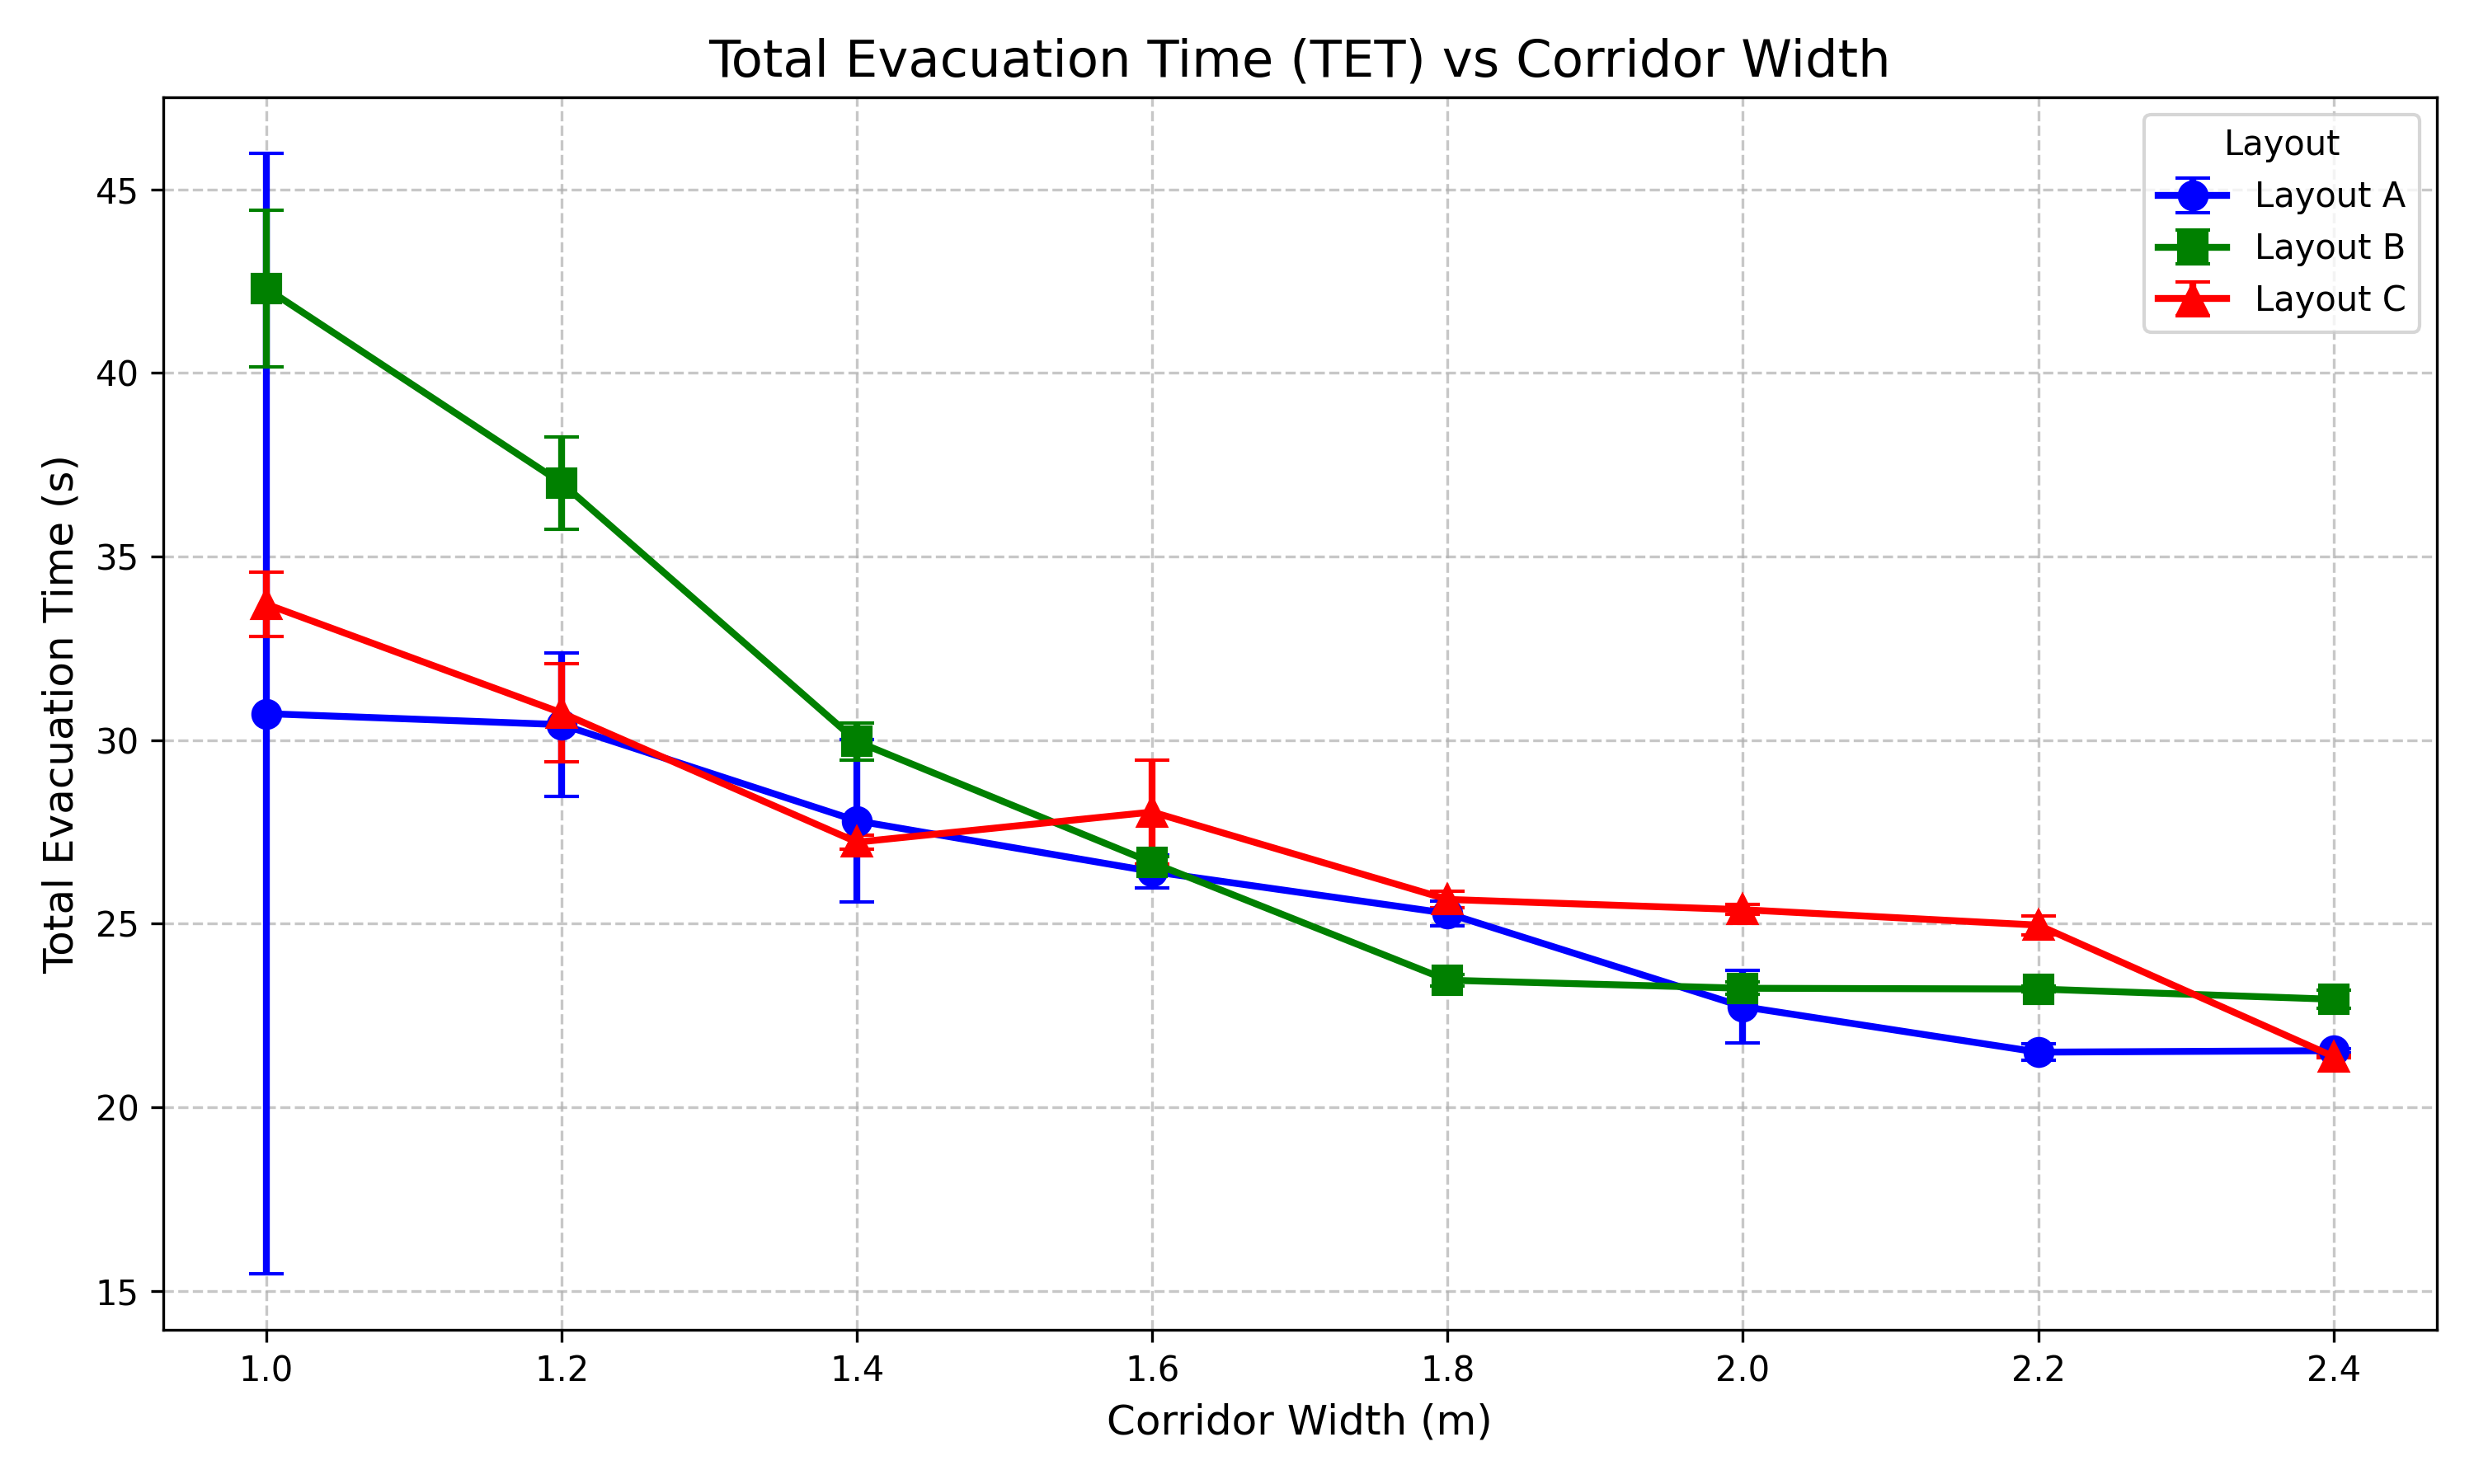
\includegraphics[width=\textwidth]{tet_vs_width.png}
    \caption{TET vs Corridor Width}
    \label{fig:tet_vs_width}
\end{figure}
The results of this study \ref{fig:tet_vs_width} indicate that the wider the corridor, the shorter the total evacuation time, but the returns from widening do not increase linearly. Within the range of approximately 1.0-1.6/1.8 m, even a slight increase in width can lead to a significant reduction in time; when the width approaches or exceeds 2.0 m, continued widening still provides benefits, but the magnitude is no longer substantial. This aligns with everyday experience: in very crowded spaces, even a small additional passageway can help disperse the flow of people; however, when the space is not particularly crowded to begin with, adding more passageway does not yield such noticeable improvement.

\subsection{Speed and Trajectories Analysis}
Looking at the speed and trajectories of Layout A \ref{fig:speed_trajectory_layout_A},B \ref{fig:speed_trajectory_layout_B},C \ref{fig:speed_trajectory_layout_C}, as the width increased from 1.0m to 1.6-1.8m, the main corridors of the three layouts generally transformed from a crowded zone to two relatively stable parallel lanes. The speed chart shows that the originally continuous red and yellow bands have been replaced by two greener bands, and the slow zone has significantly contracted. This indicates that the increase in width first reduces lateral friction and frequent evasive maneuvering, allowing individuals to maintain a speed close to free-flow for a longer period of time. In terms of the total evacuation time, this stage has the largest reduction, and the result fluctuations of each layout have simultaneously decreased.
\begin{figure}[h]
    \centering
    \includegraphics[width=\textwidth]{speed_trajectory_layout_A.png}
    \caption{Speed and Trajectories for Layout A}
    \label{fig:speed_trajectory_layout_A}
\end{figure}
\\The main corridor in Layout A is relatively straight, with multiple tributary inflow points along the line. The trajectory and velocity diagrams show that tributaries have already formed orderly queues before reaching the confluence point, with only mild short-distance deceleration when entering the main corridor. This suggests that conflicts are resolved in advance within the tributaries, with stable dual lanes forming starting from corridor widths of 1.6 m, while widths of 2.0-2.4 m maintain only small deceleration zones before the final exit. As a result, medium to high-width sections have lower average times, smaller variances, and higher speed limits. Furthermore, as width increases, evacuation time decreases relatively steadily.
\begin{figure}[h]
    \centering
    \includegraphics[width=\textwidth]{speed_trajectory_layout_B.png}
    \caption{Speed and Trajectories for Layout B}
    \label{fig:speed_trajectory_layout_B}
\end{figure}
\\Layout B contains multiple T-shaped or cross intersections with dispersed confluence points. Under corridor widths of 1.0-1.4 m, the lower section near intersection points repeatedly experiences team breaking and regrouping phenomena. The visual manifestation in the diagram is the formation of multiple mesh-like low-speed zones, with numerous congestion points covering a wide range. After widening the width to 1.6 and 1.8 m, these mesh-like low-speed zones significantly diminish and form lanes, which indicates that widening the corridor width can effectively avoid interactive conflicts, resulting in the greatest time reduction. However, at 2.4 m, some remaining light yellow zones are still visible, causing the speed limitation at the high-width stage to be slightly lower than layouts A and C.
\begin{figure}[h]
    \centering
    \includegraphics[width=\textwidth]{speed_trajectory_layout_C.png}
    \caption{Speed and Trajectories for Layout C}
    \label{fig:speed_trajectory_layout_C}
\end{figure}
\\Layout C \ref{fig:speed_trajectory_layout_C} employs parallel lanes upstream, which allows agents to form queues before merging into the main corridor, showing better organization than Layout B. However, merging still requires navigating through a turning angle, resulting in a relatively low overall speed limitation. As shown in \ref{fig:tet_vs_width}, Layout C exhibits an abnormal fluctuation at 1.6 m width, where evacuation time is actually longer than that of the 1.4 m corridor width. Comparing the speed and trajectory diagrams for 1.4 m and 1.6 m cases, we can observe that in the 1.6 m scenario, although attempts are made to form two lanes in the bottleneck area before the exit and the merging zone below, the centerline distance between the two lanes remains too close. This intuisively results in a great increase in lane width, reflecting more friction and avoidance behavior, which matches the Social Force Model's description. After the width increases to 1.8-2.0 m, the inter-lane spacing and merging diffusion angle increase, the slow-speed zones are eliminated, and evacuation performance rapidly improves. At the width of 2.4 m , the turning angle effect becomes essentially negligible, and the speed limitation exceeded that of Layout A.
\\Among the three layout types, stable low-speed zones most commonly appear at the following locations: intersections or merging areas, sharp turns and convergence sections before exits. Increasing width makes these low-speed zones shorter, shallower and less frequent. This may indicate that corridor width is not a direct contributing factor. Rather than continuing to widen corridors blindly when the corridor width is already relatively wide, it would be better to optimize these low-speed zones, such as extending merging transitions, reducing merge angles and increasing directional guidance and one-way organization.

\subsection{Double Exits Comparison}
According to Figure \ref{fig:all_tet_vs_width}, after setting up dual exits, the total evacuation time for all three layouts decreased overall, with significantly reduced fluctuation between trials. The 1.0-1.6/1.8 m range remains the interval with the fastest efficiency improvement; when the width beyond 2.0 m, the marginal benefits of continued widening disappear, and the curve tends to flatten. Compared to single exit, double exits first reduce the low-speed zones in the terminal convergence section, offering the system a stable state with sufficient capacity. Under double exits condition, the speed and trajectories of all three layouts are more uniform and the trend is smooth, with significantly more green sections, while red and yellow low-speed zones are compressed into shorter localized areas. Agents seperate earlier after they start to evacute, and the backtracking and snake-like movement in the main corridor are notably reduced.
\begin{figure}[h]
    \centering
    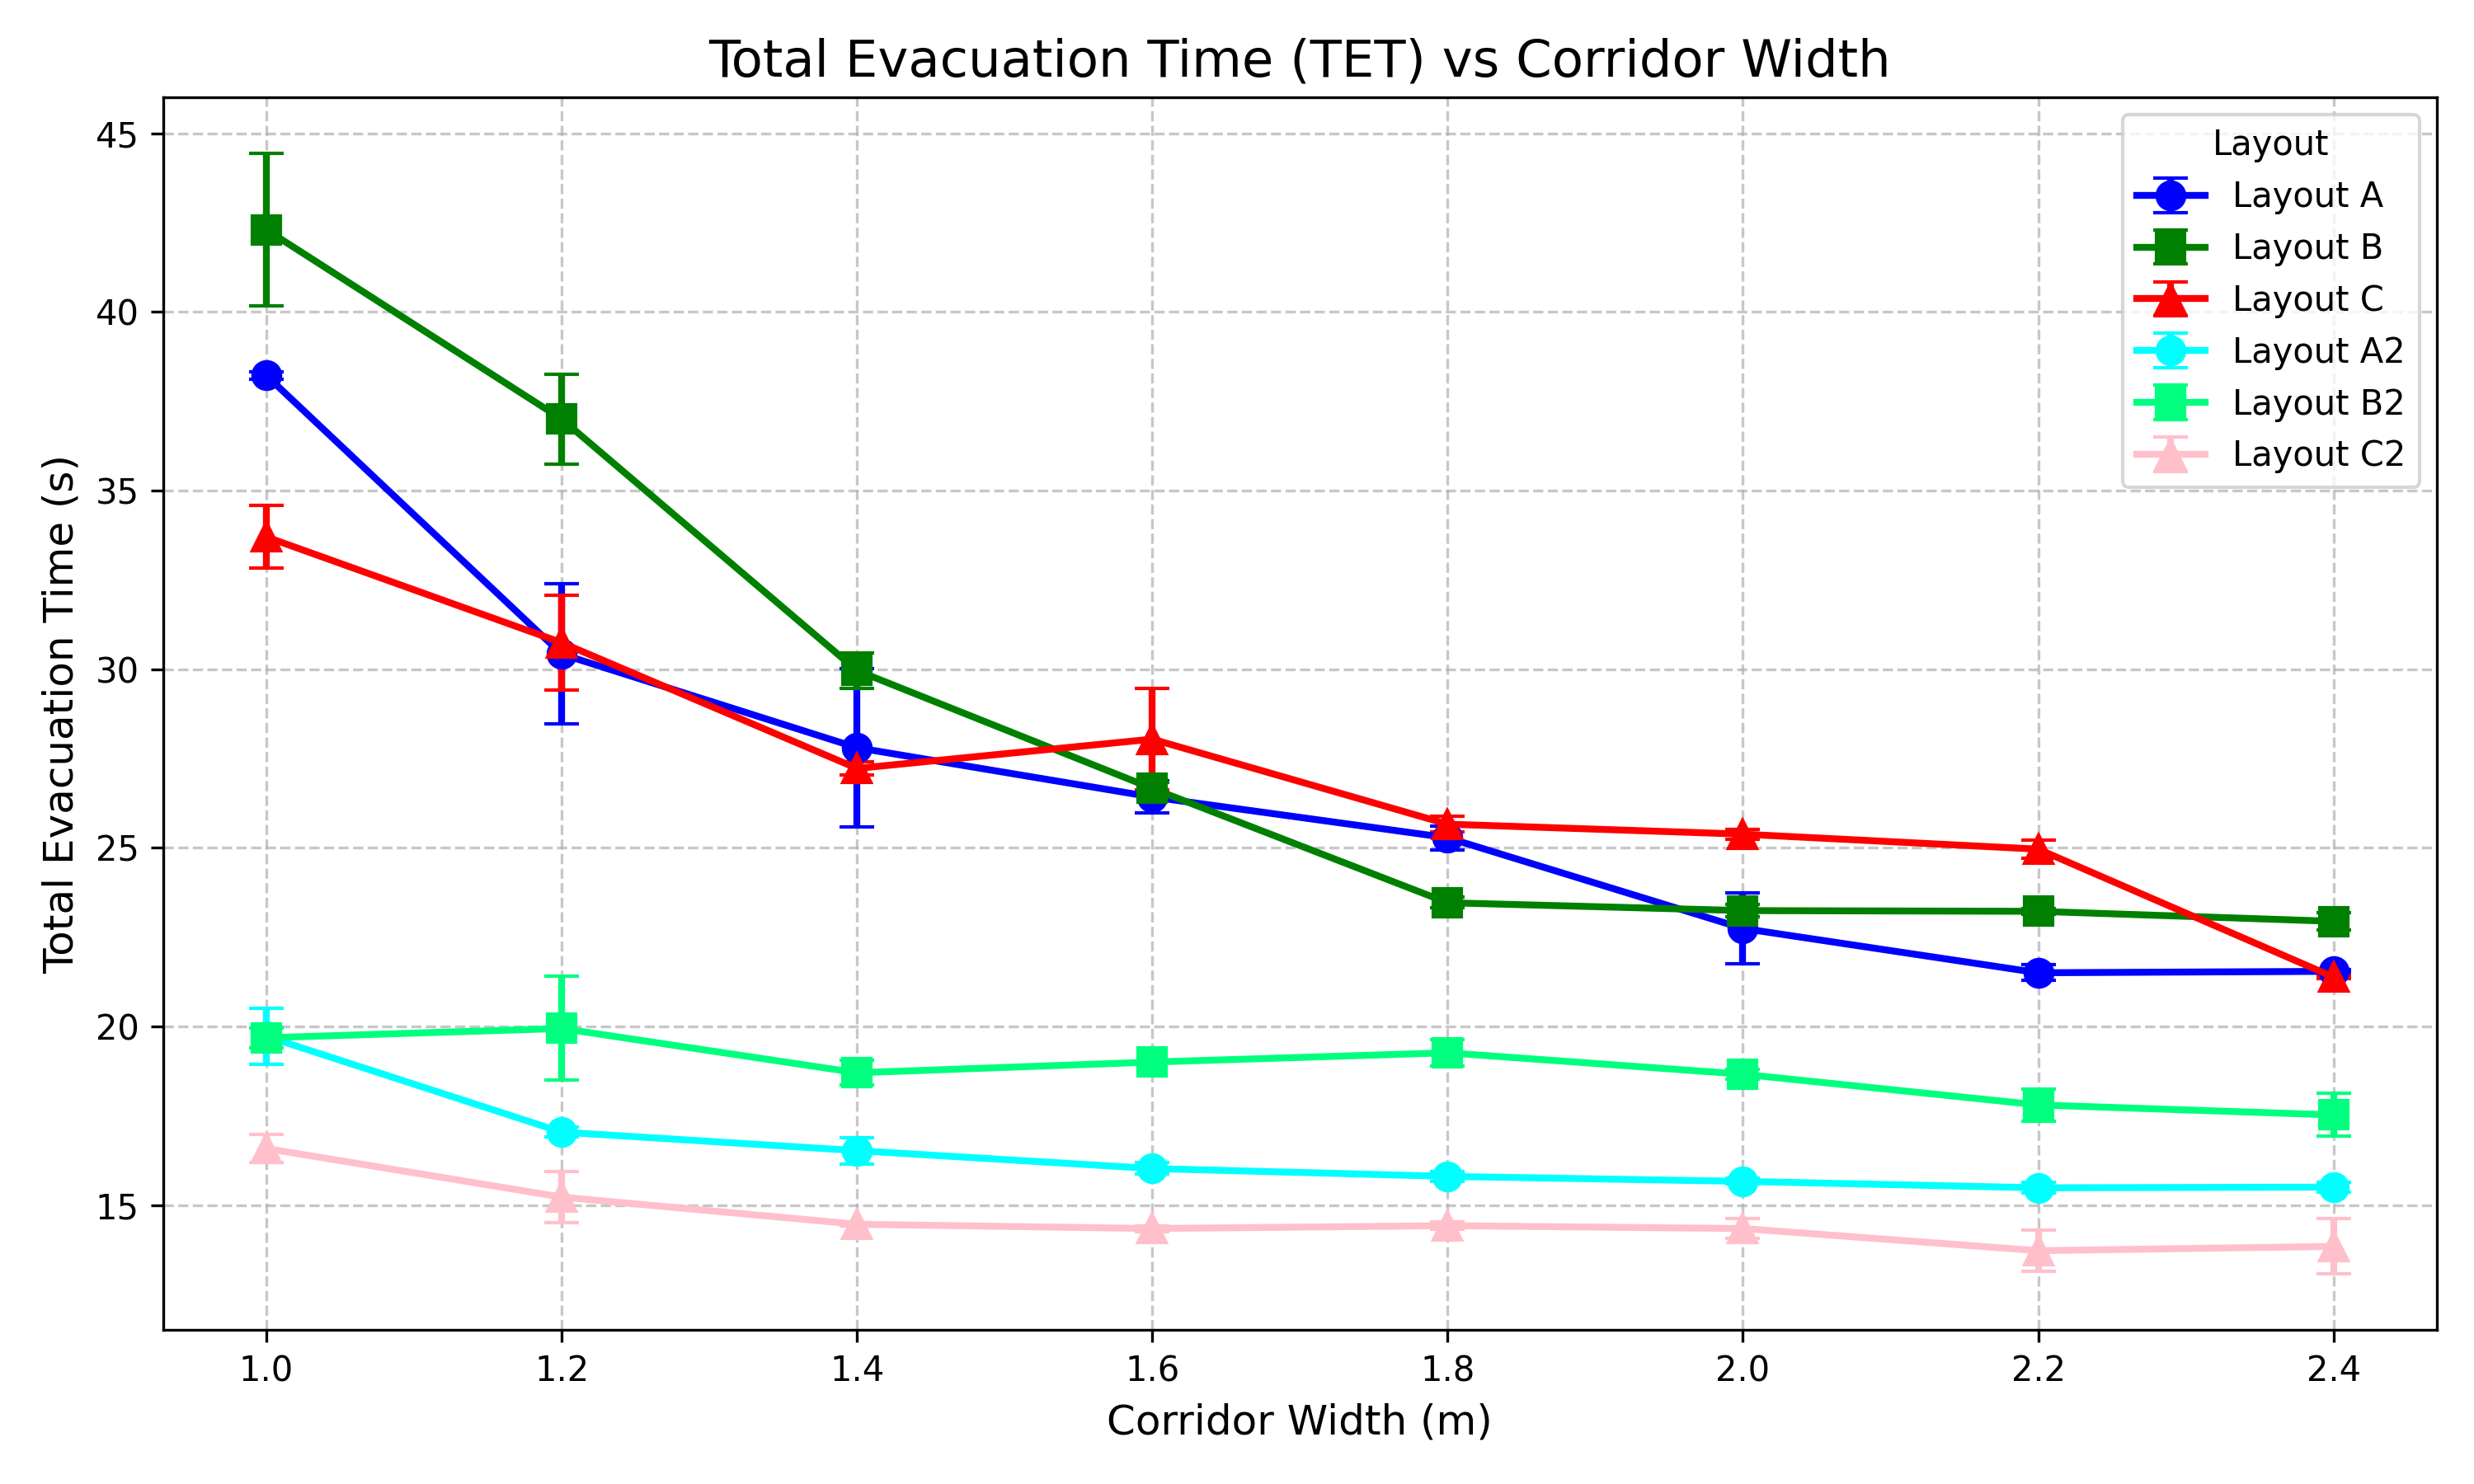
\includegraphics[width=\textwidth]{All_tet_vs_width.png}
    \caption{TET vs Corridor Width for All Layouts with Single and Double Exits}
    \label{fig:all_tet_vs_width}
\end{figure}

\begin{figure}[h]
    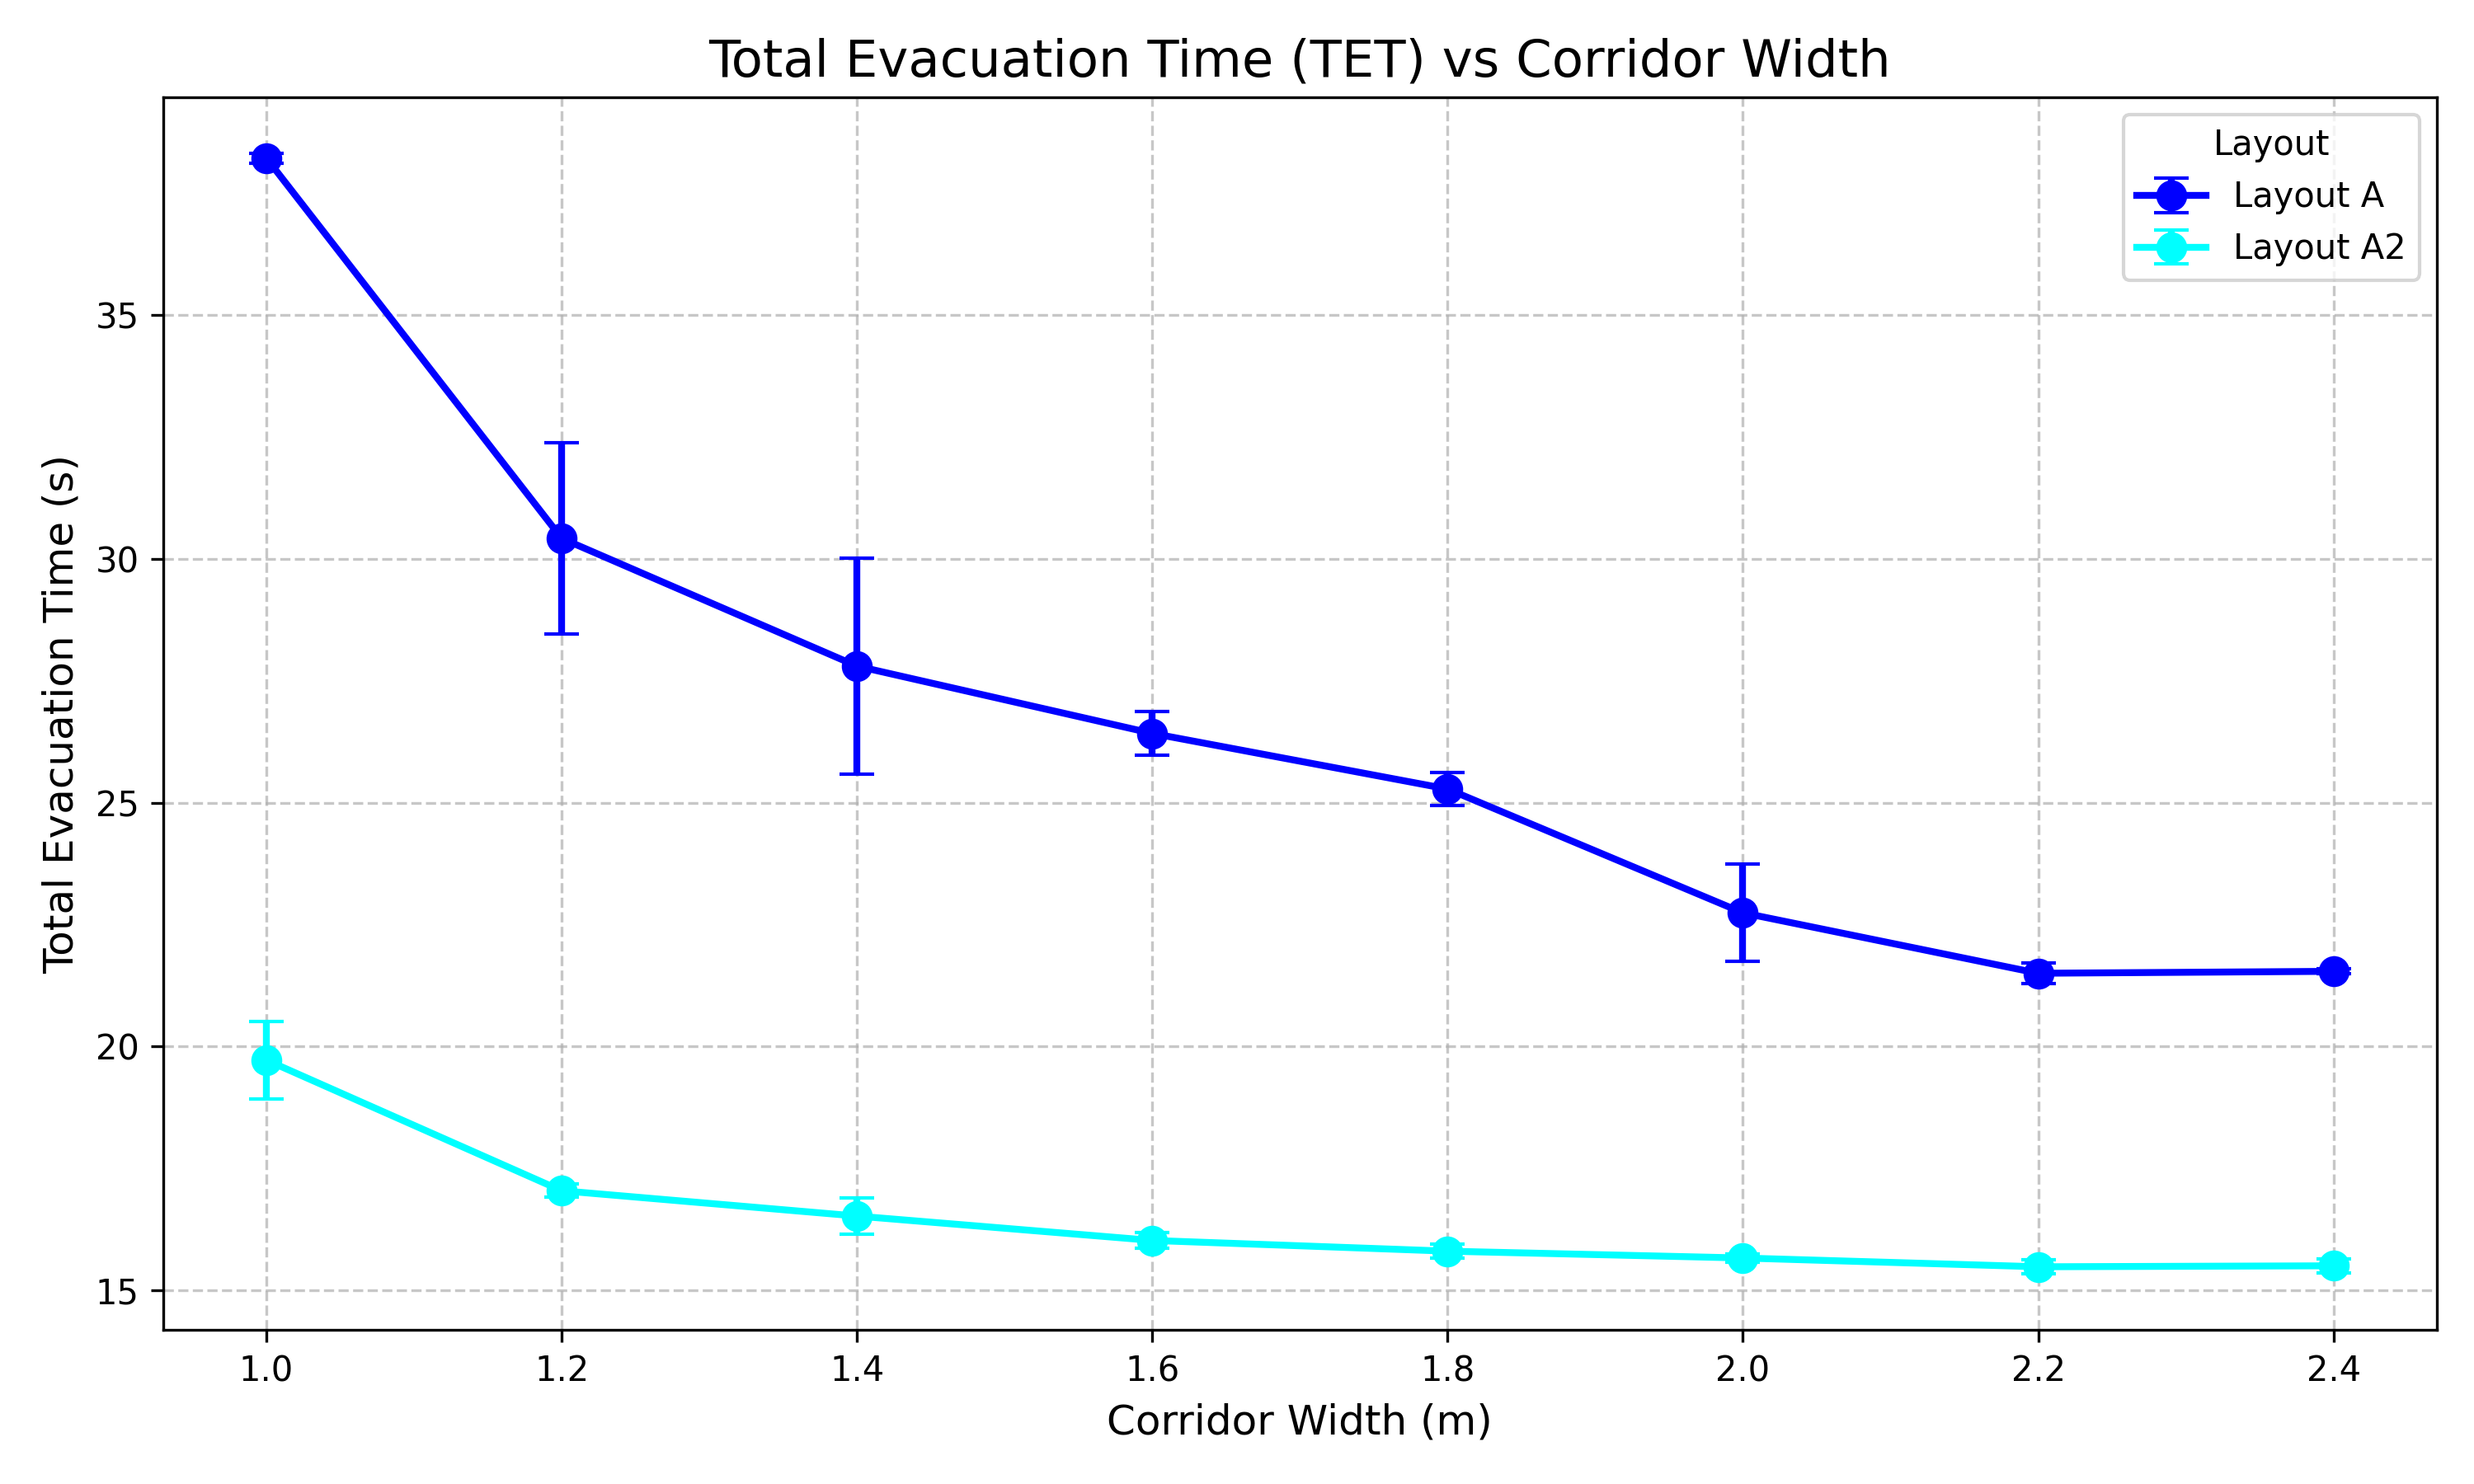
\includegraphics[width=\linewidth]{AvsA2_tet_vs_width.png}
    \caption{TET vs Corridor Width between A and A2}\label{fig:AvsA2_tet_vs_width}
\end{figure}

\begin{figure}[h]
    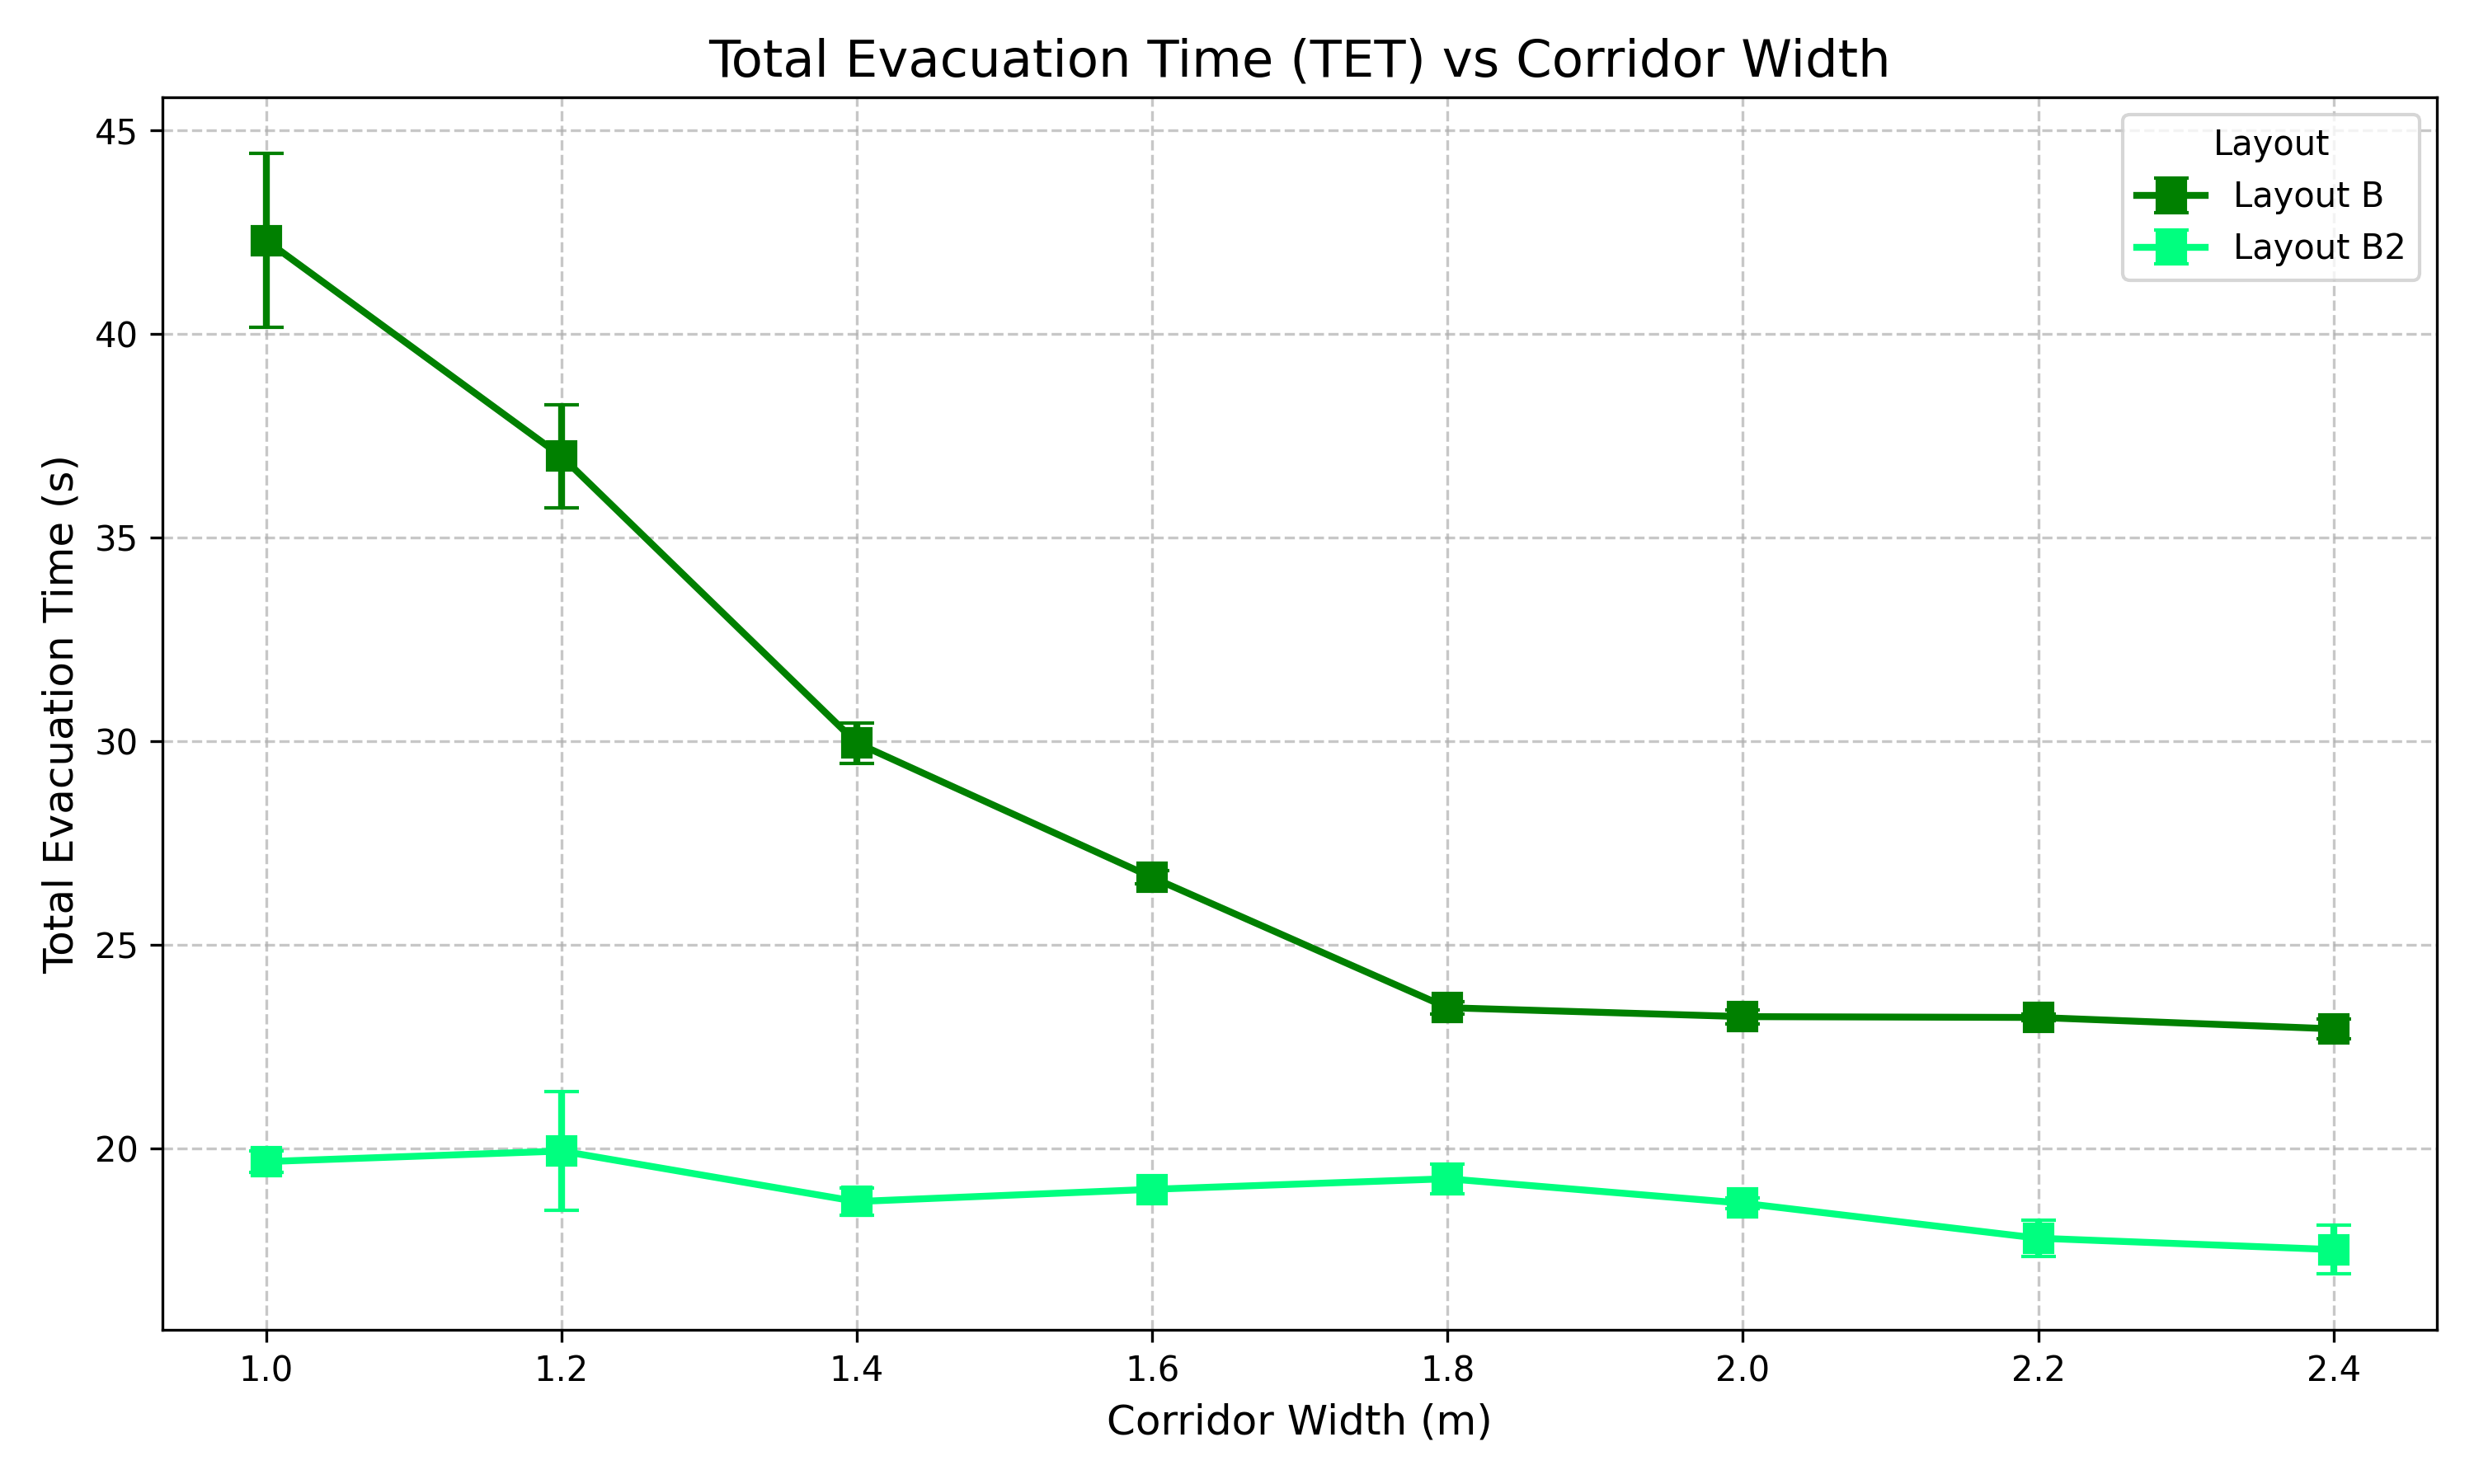
\includegraphics[width=\linewidth]{BvsB2_tet_vs_width.png}
    \caption{TET vs Corridor Width between B and B2}\label{fig:BvsB2_tet_vs_width}
\end{figure}

\begin{figure}[h]
    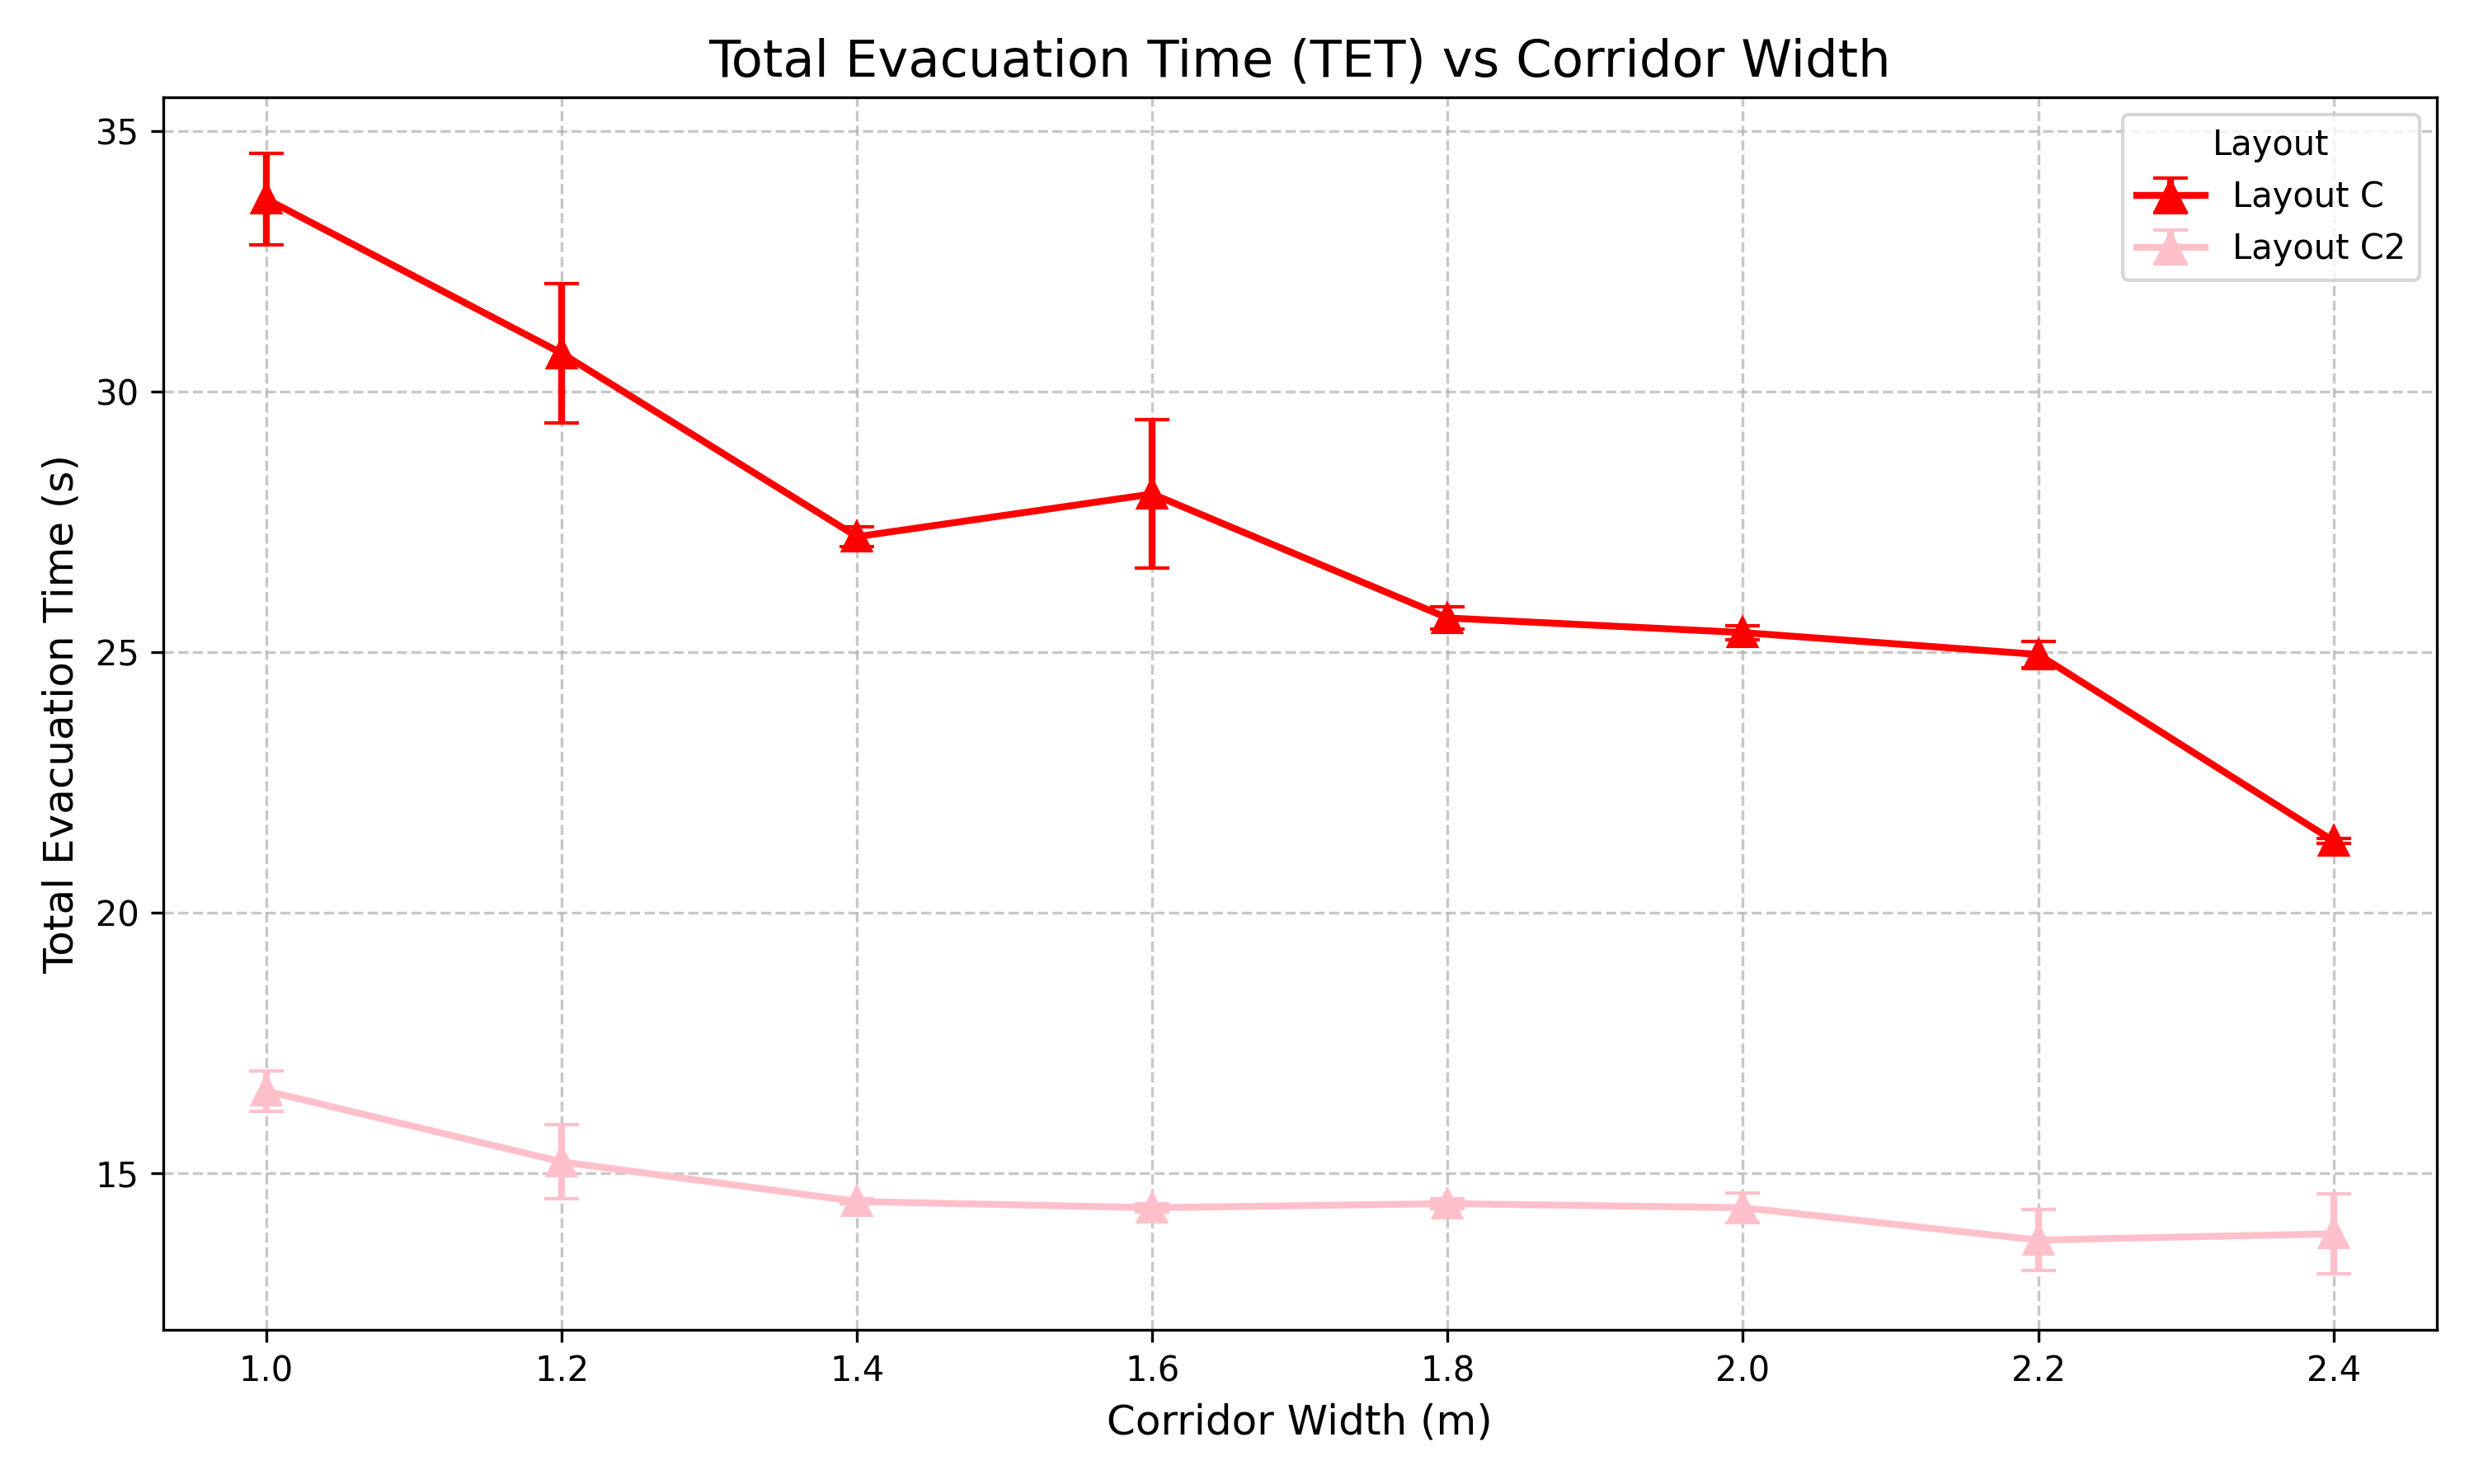
\includegraphics[width=\linewidth]{CvsC2_tet_vs_width.png}
    \caption{TET vs Corridor Width between C and C2}\label{fig:CvsC2_tet_vs_width}
\end{figure}
Under single exit condition, Layout A \ref{fig:speed_trajectory_layout_A} can easily form a continuous low-speed zone before the exit. Although relatively stable double lanes have appeared in the middle section, the convergence of lanes at the end still causes significant speed reduction and creates certain fluctuations. When it comes to double exits \ref{fig:speed_trajectory_layout_A2}, the flow distribution shifts the merging points towards both side exits, weakening the low-speed zone and leaving deceleration before merging. The trajectories show almost no congestion or fluctuation, with the main green flow band extending throughout the entire length. The result shows that the Layout A2 maintains low and stable total times across all widths, showing that the double-exit design directly eliminates the terminal bottleneck.
\begin{figure}[h]
    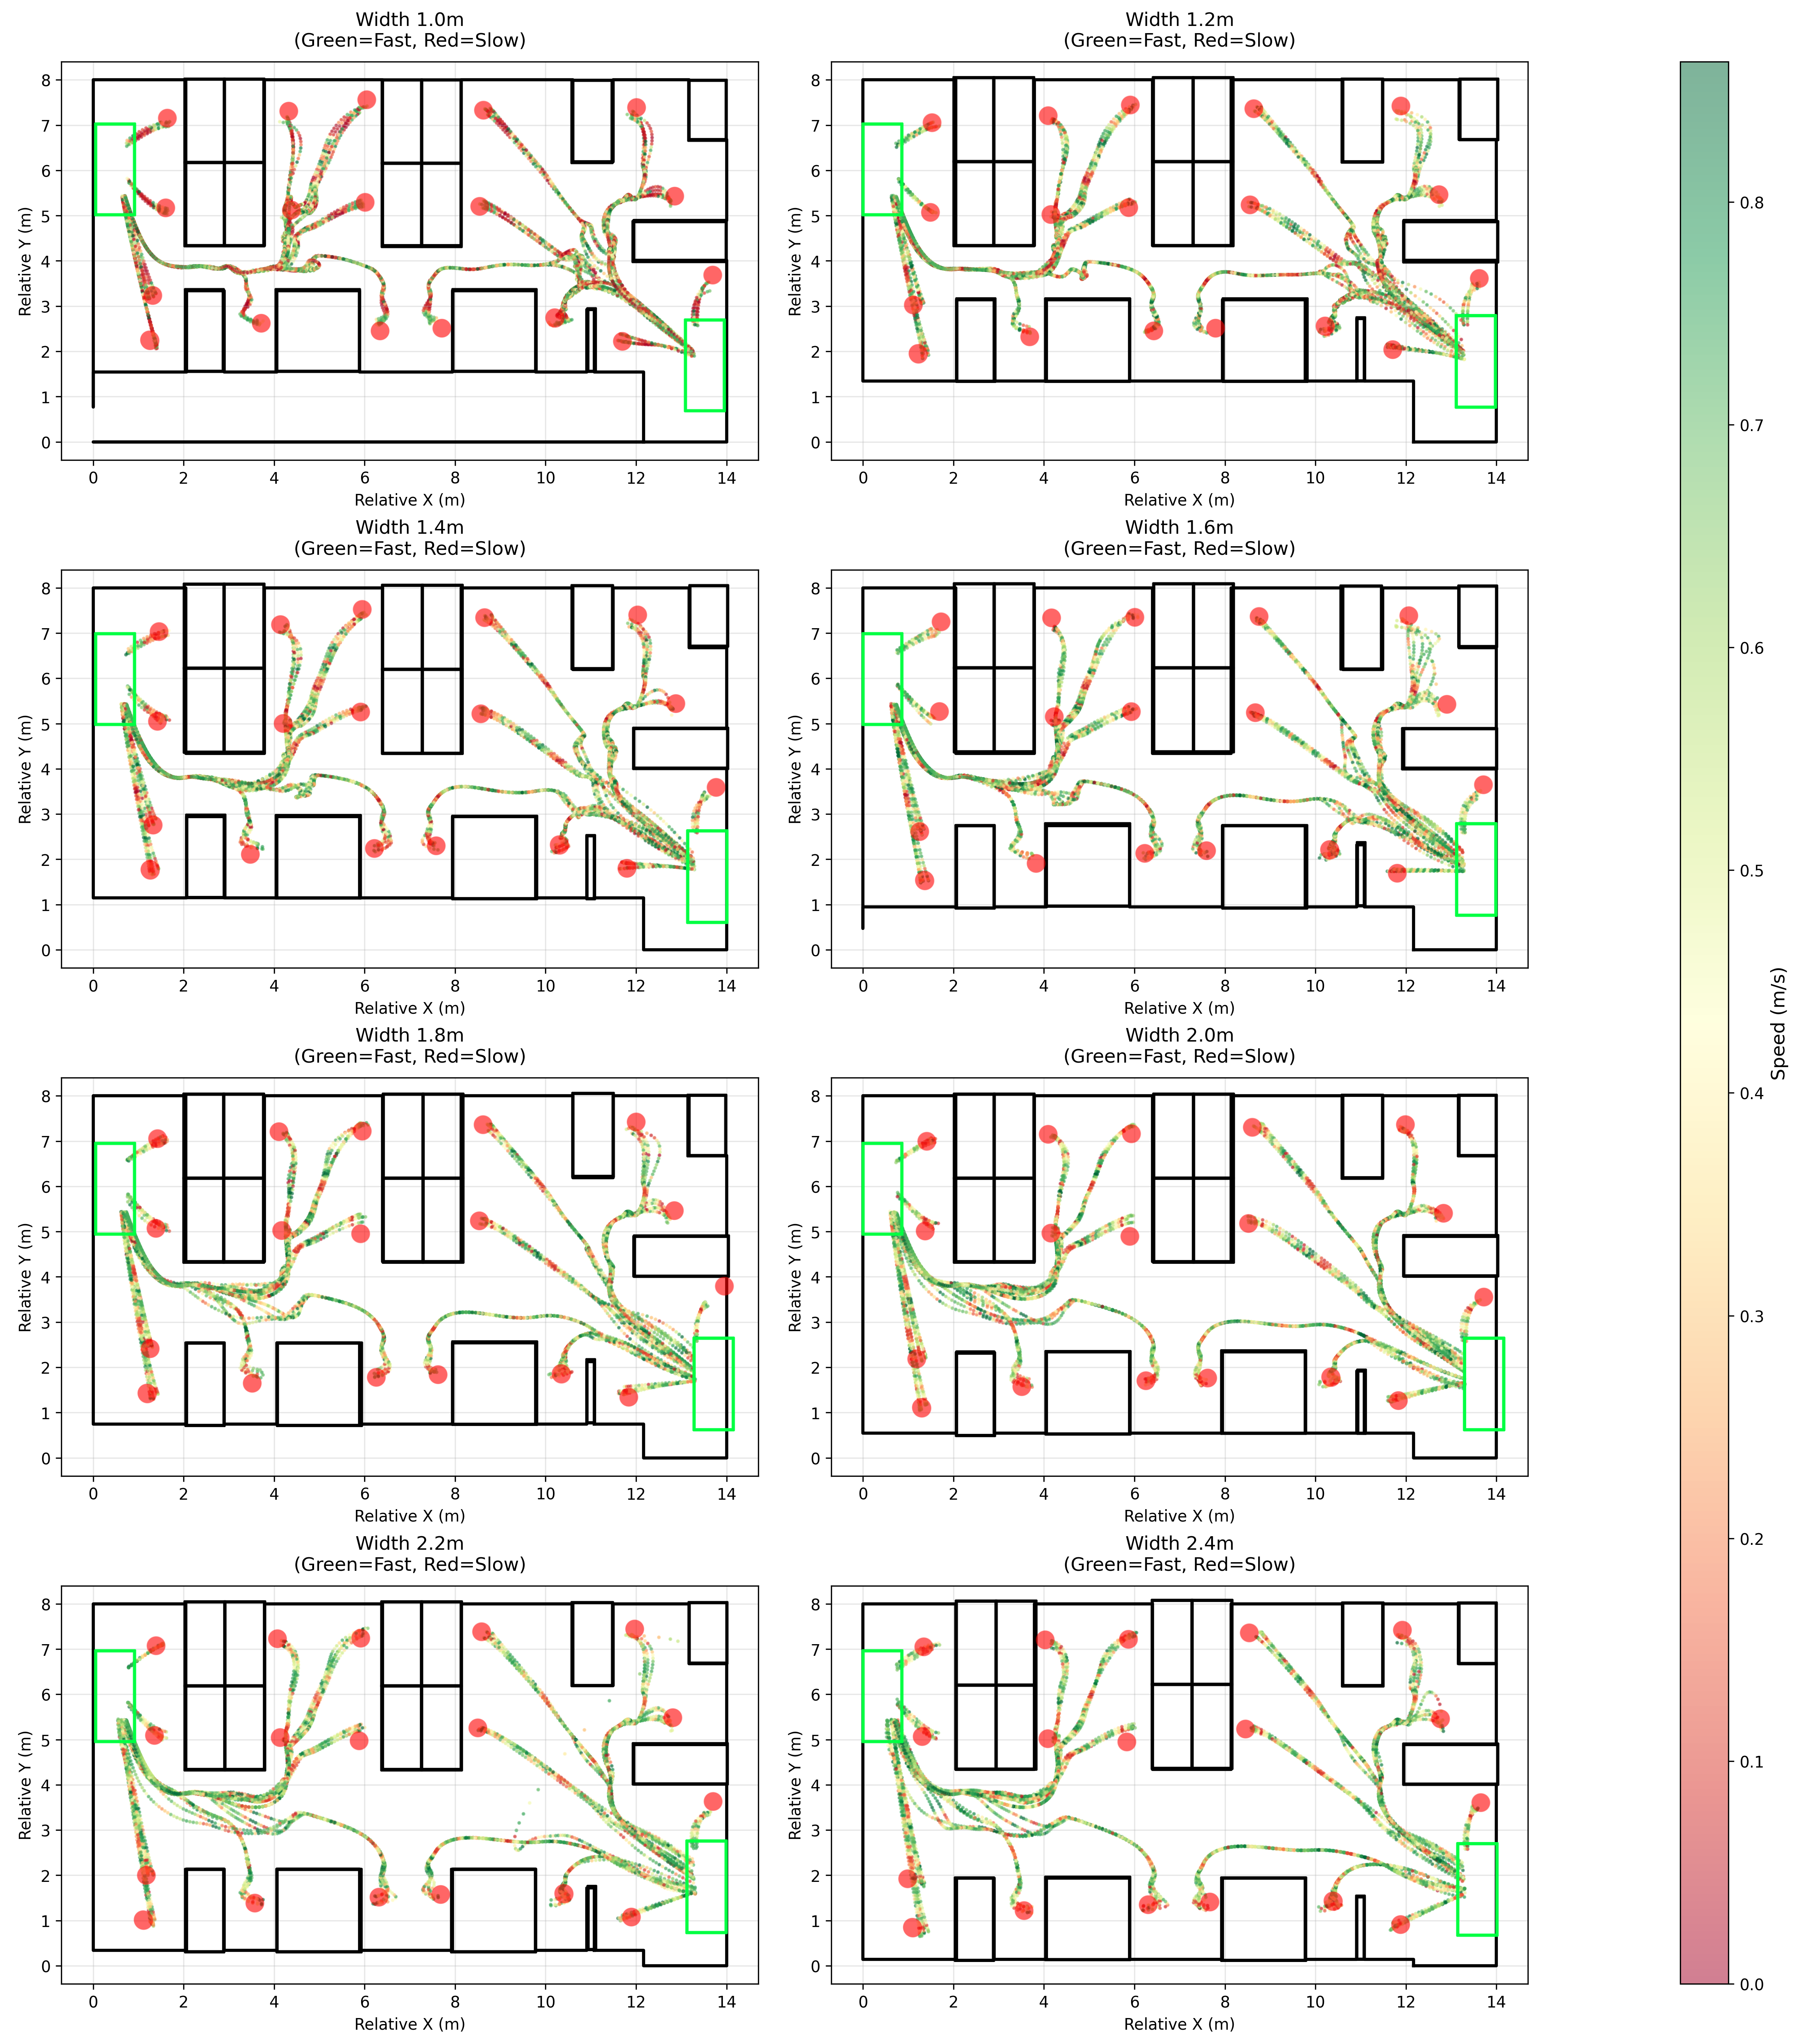
\includegraphics[width=\linewidth]{speed_trajectory_layout_A2.png}
    \caption{Speed and Trajectories for Layout A2}\label{fig:speed_trajectory_layout_A2}
\end{figure}
\\In single-exit Layout B \ref{fig:speed_trajectory_layout_B}, repeated phenomena of crowd breakup and regrouping occur near multiple intersections, forming a network of red and yellow slow-speed zones on the speed diagram, particularly prominent in the 1.0-1.4 m range. After introducing the second exit \ref{fig:speed_trajectory_layout_B2}, the terminal convergence pressure in Layout B2 was not significantly reduced, with only slight decreases in evacuation time, and even increases in time observed in the condition of 1.2m and 1.4-1.8m corridor width. The reason may be that multiple intersection points are still retained in the upper zone of the area, requiring agents to make multiple detours and reorganizations. The two-sided flow distribution and widened passages cannot effectively alleviate congestion at these local intersection points. Meanwhile, the wider passages may actually make agents' avoidance behavior more pronounced, thereby slowing down evacuation time. This indicates that for geometries with dense intersections, although double exits can alleviate terminal congestion, further reduction of low-speed zones still requires local geometric modification measures.
\begin{figure}[h]
    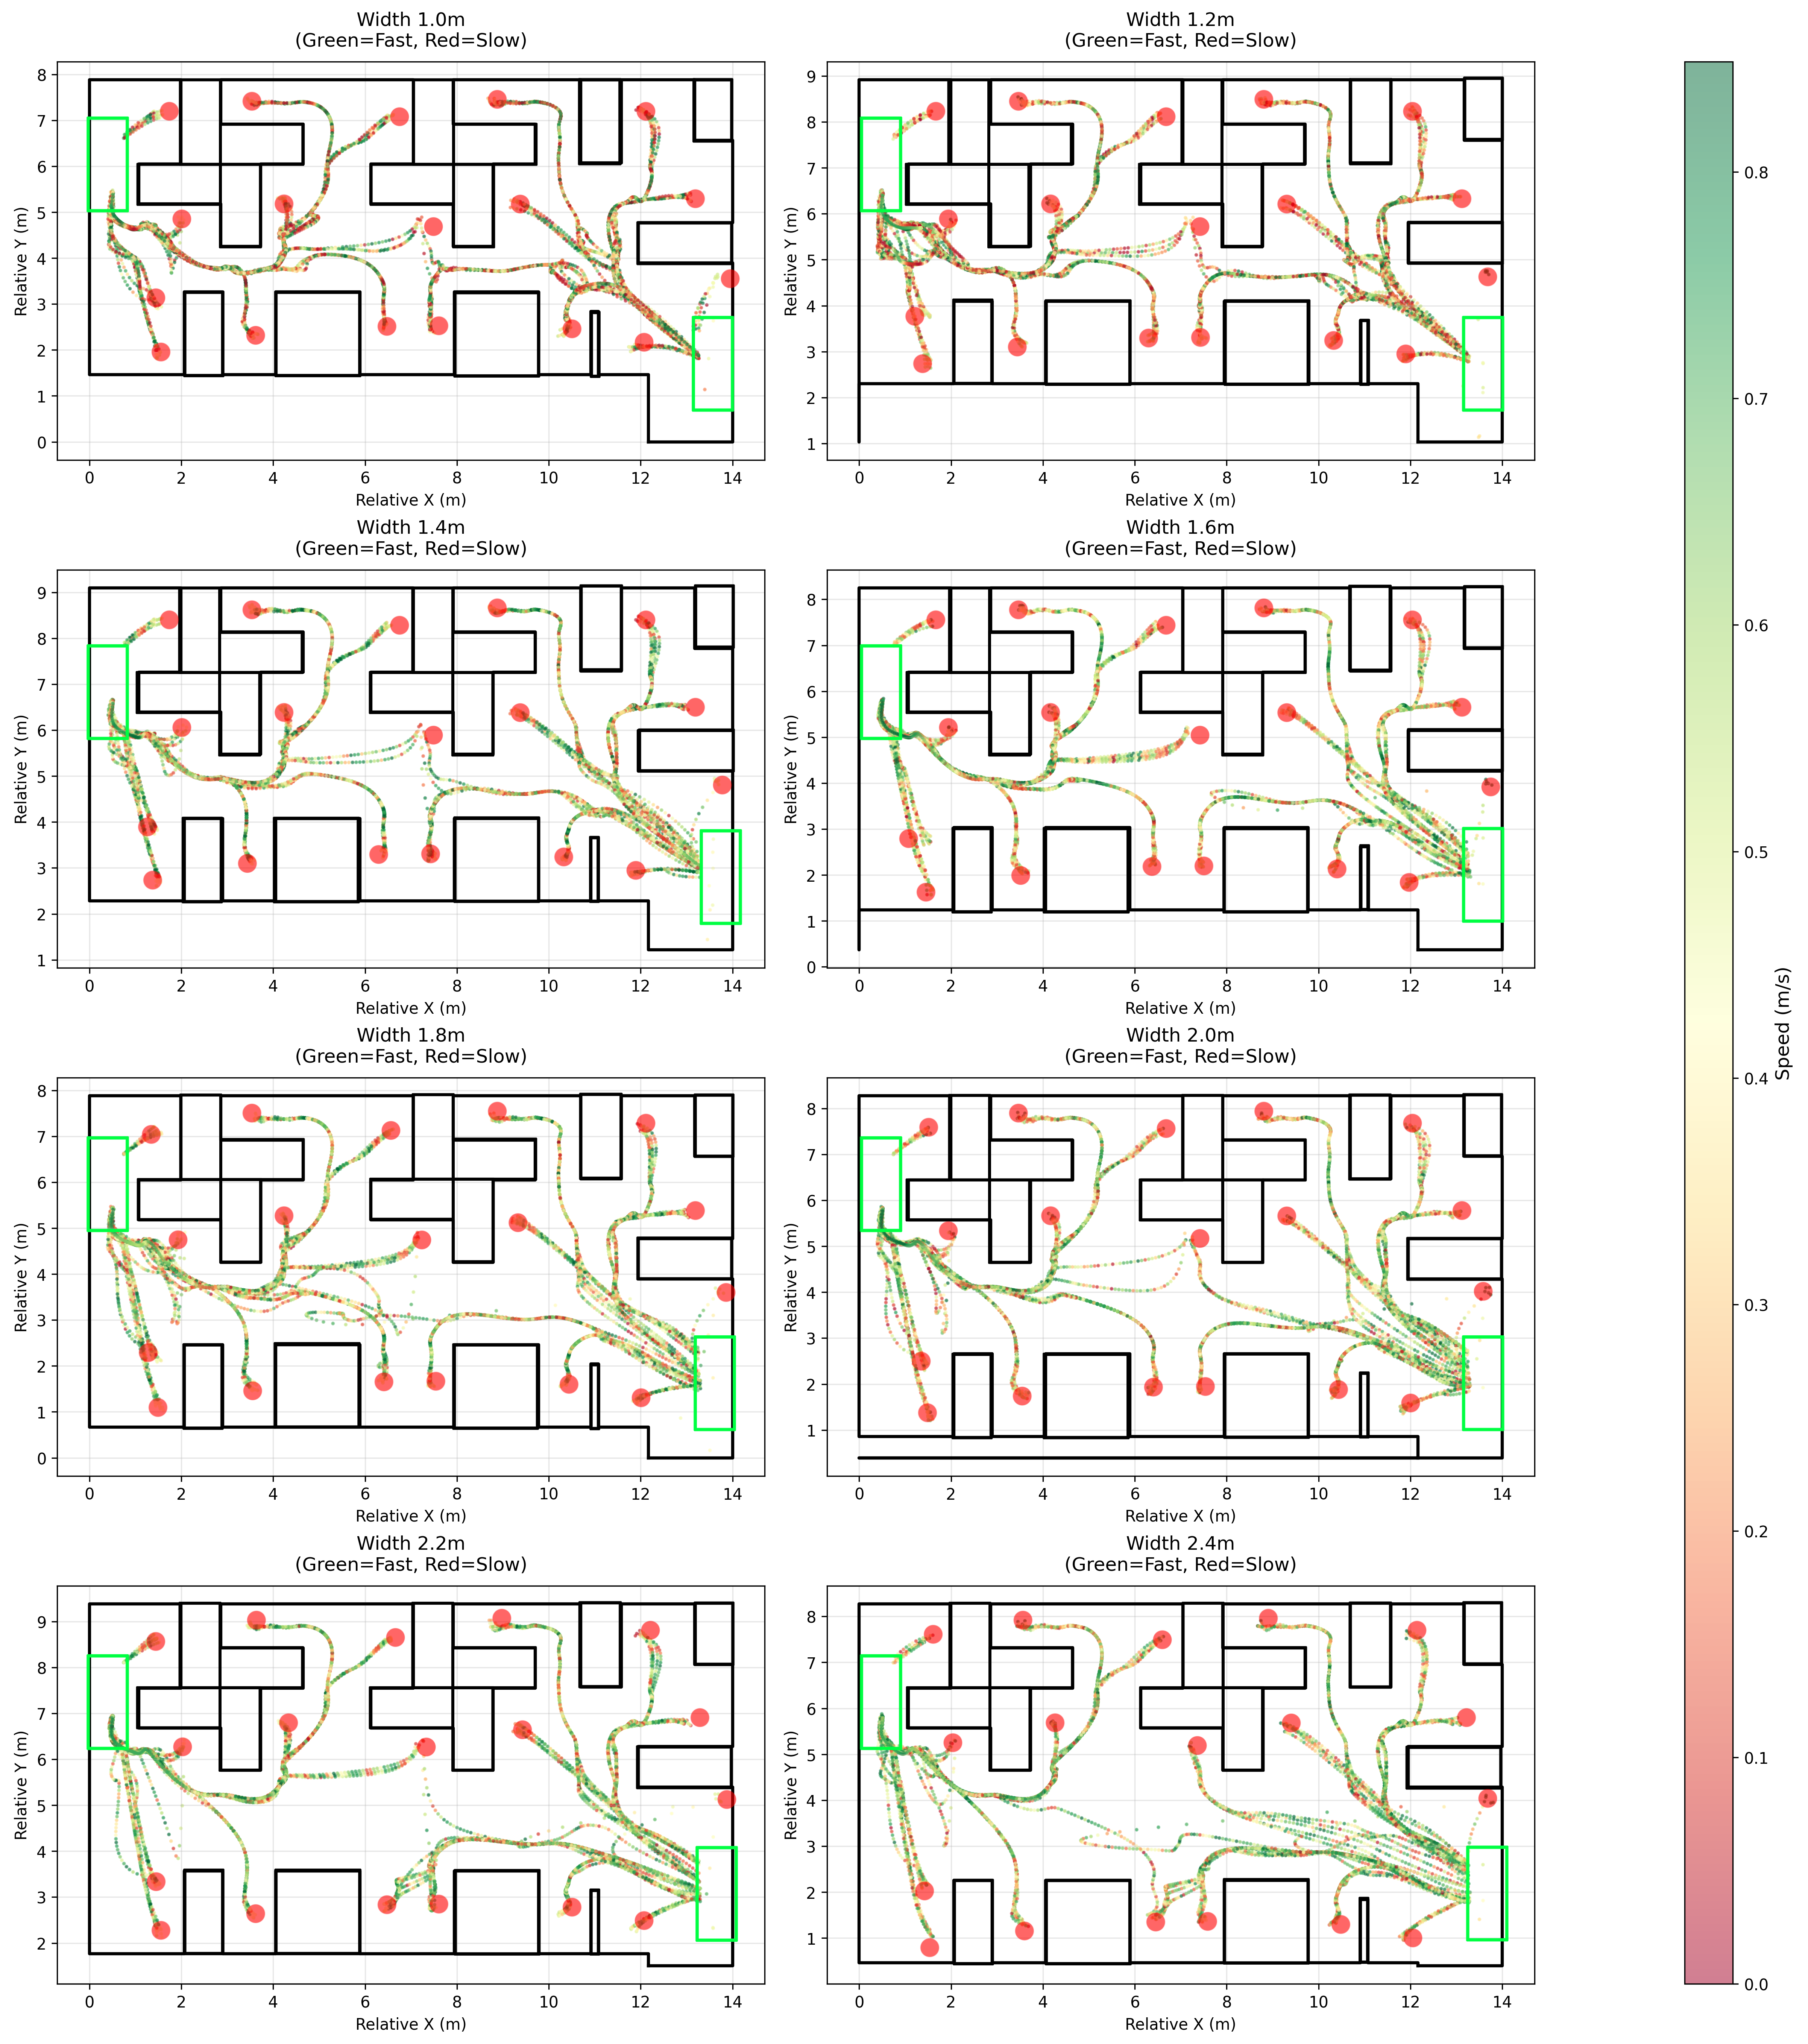
\includegraphics[width=\linewidth]{speed_trajectory_layout_B2.png}
    \caption{Speed and Trajectories for Layout B2}\label{fig:speed_trajectory_layout_B2}
\end{figure}
\\In single-exit Layout C \ref{fig:speed_trajectory_layout_C}, the parallel chnnels in the upper zone can form orderly queues in advance, but continuous low-speed zones appear at the corner. After setting up double exits \ref{fig:speed_trajectory_layout_C2}, the queues formed in the upper zone can be released directly through the upper-left exit without needing to pass through the corner and merge into the main corridor. This allows the Layout C2 to have the lowest overall evacuation time across all widths. This indicates that the double exits effectively weakened the influence of corner and fully utilized the advantages of parallel channels.
\begin{figure}[h]
    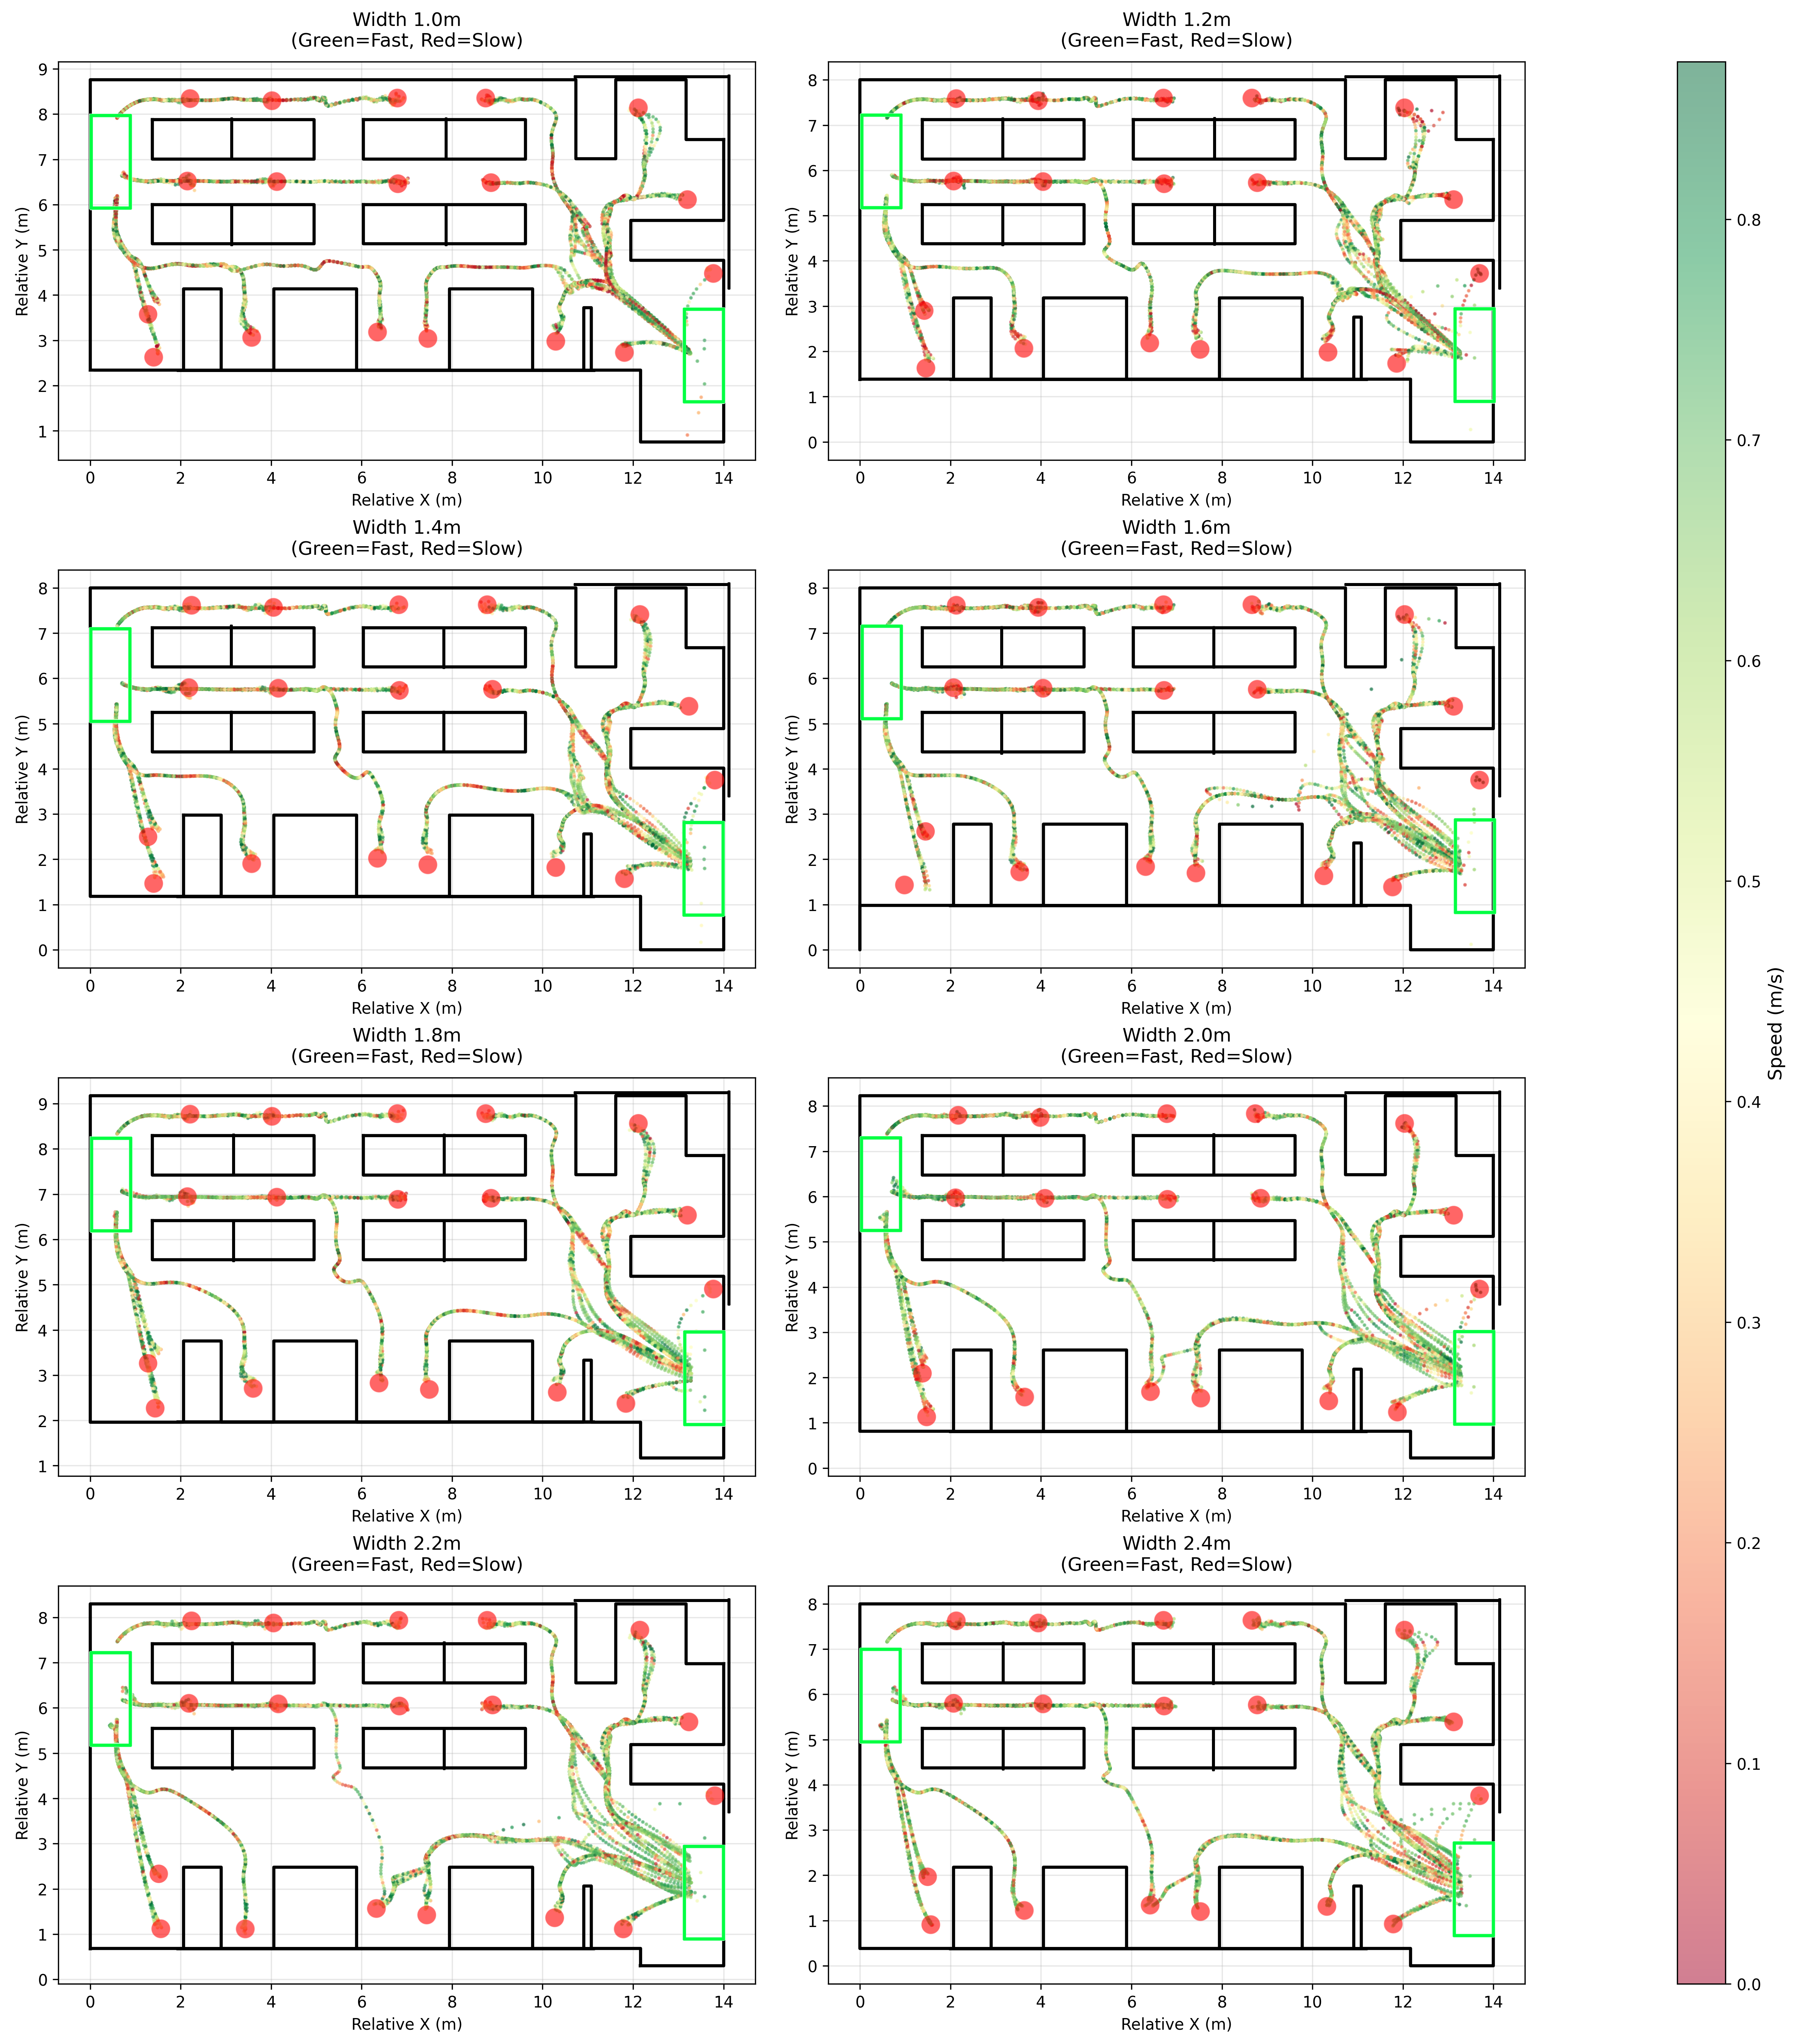
\includegraphics[width=\linewidth]{speed_trajectory_layout_C2.png}
    \caption{Speed and Trajectories for Layout C2}\label{fig:speed_trajectory_layout_C2}
\end{figure}

\section{Big Prototype}
Based on the results from the Small Prototype, evacuation time shows significant correlation with the convergence intensity at the end of main corridors, as well as mutual interference among crowds at intersections and merging points. Therefore, we introduce the Big Prototype to test these mechanisms in larger spaces and crowd scales, to examine their persistence and increase effects at the macro level, with focus on identifying the gates width and geometric threshold ranges that can most significantly infuence the total evacuation time.
\subsection{Effect of Bottleneck Width(Gate Width Before Exit)}
In the Big Prototype scenario, according to the figure \ref{fig:tet_vs_Bottleneck}, as the exit bottleneck width gradually increased from 1.0 m to 1.6 m, the Total Evacuation Time (TET) showed a continuous declining monotonic trend. The readings approximately showed 85 s at 1.0 m, 75 s at 1.2 m, 73 s at 1.4 m, and 70 s at 1.6 m. The most significant improvement occurred in the interval from 1.0 m to 1.2 m, where TET decreased by approximately 10 s with nearly a twelve percent relative improvement; thereafter, continued widening only brought gradual improvements, with approximately 2 s reduction in the 1.2 m to 1.4 m interval and approximately 3 s reduction in the 1.4 m to 1.6 m interval. Error bars showed that the variability of repeated runs was greater at narrower exits and significantly converged at wider exits, indicating that the system was more stable at larger widths. The slope of the line showed a noticeable change around 1.2 m, suggesting that this point may be the threshold interval for transitioning from long queue formation to short-term congestion, beyond which marginal benefits gradually diminish.
\begin{figure}[h]
    \centering
    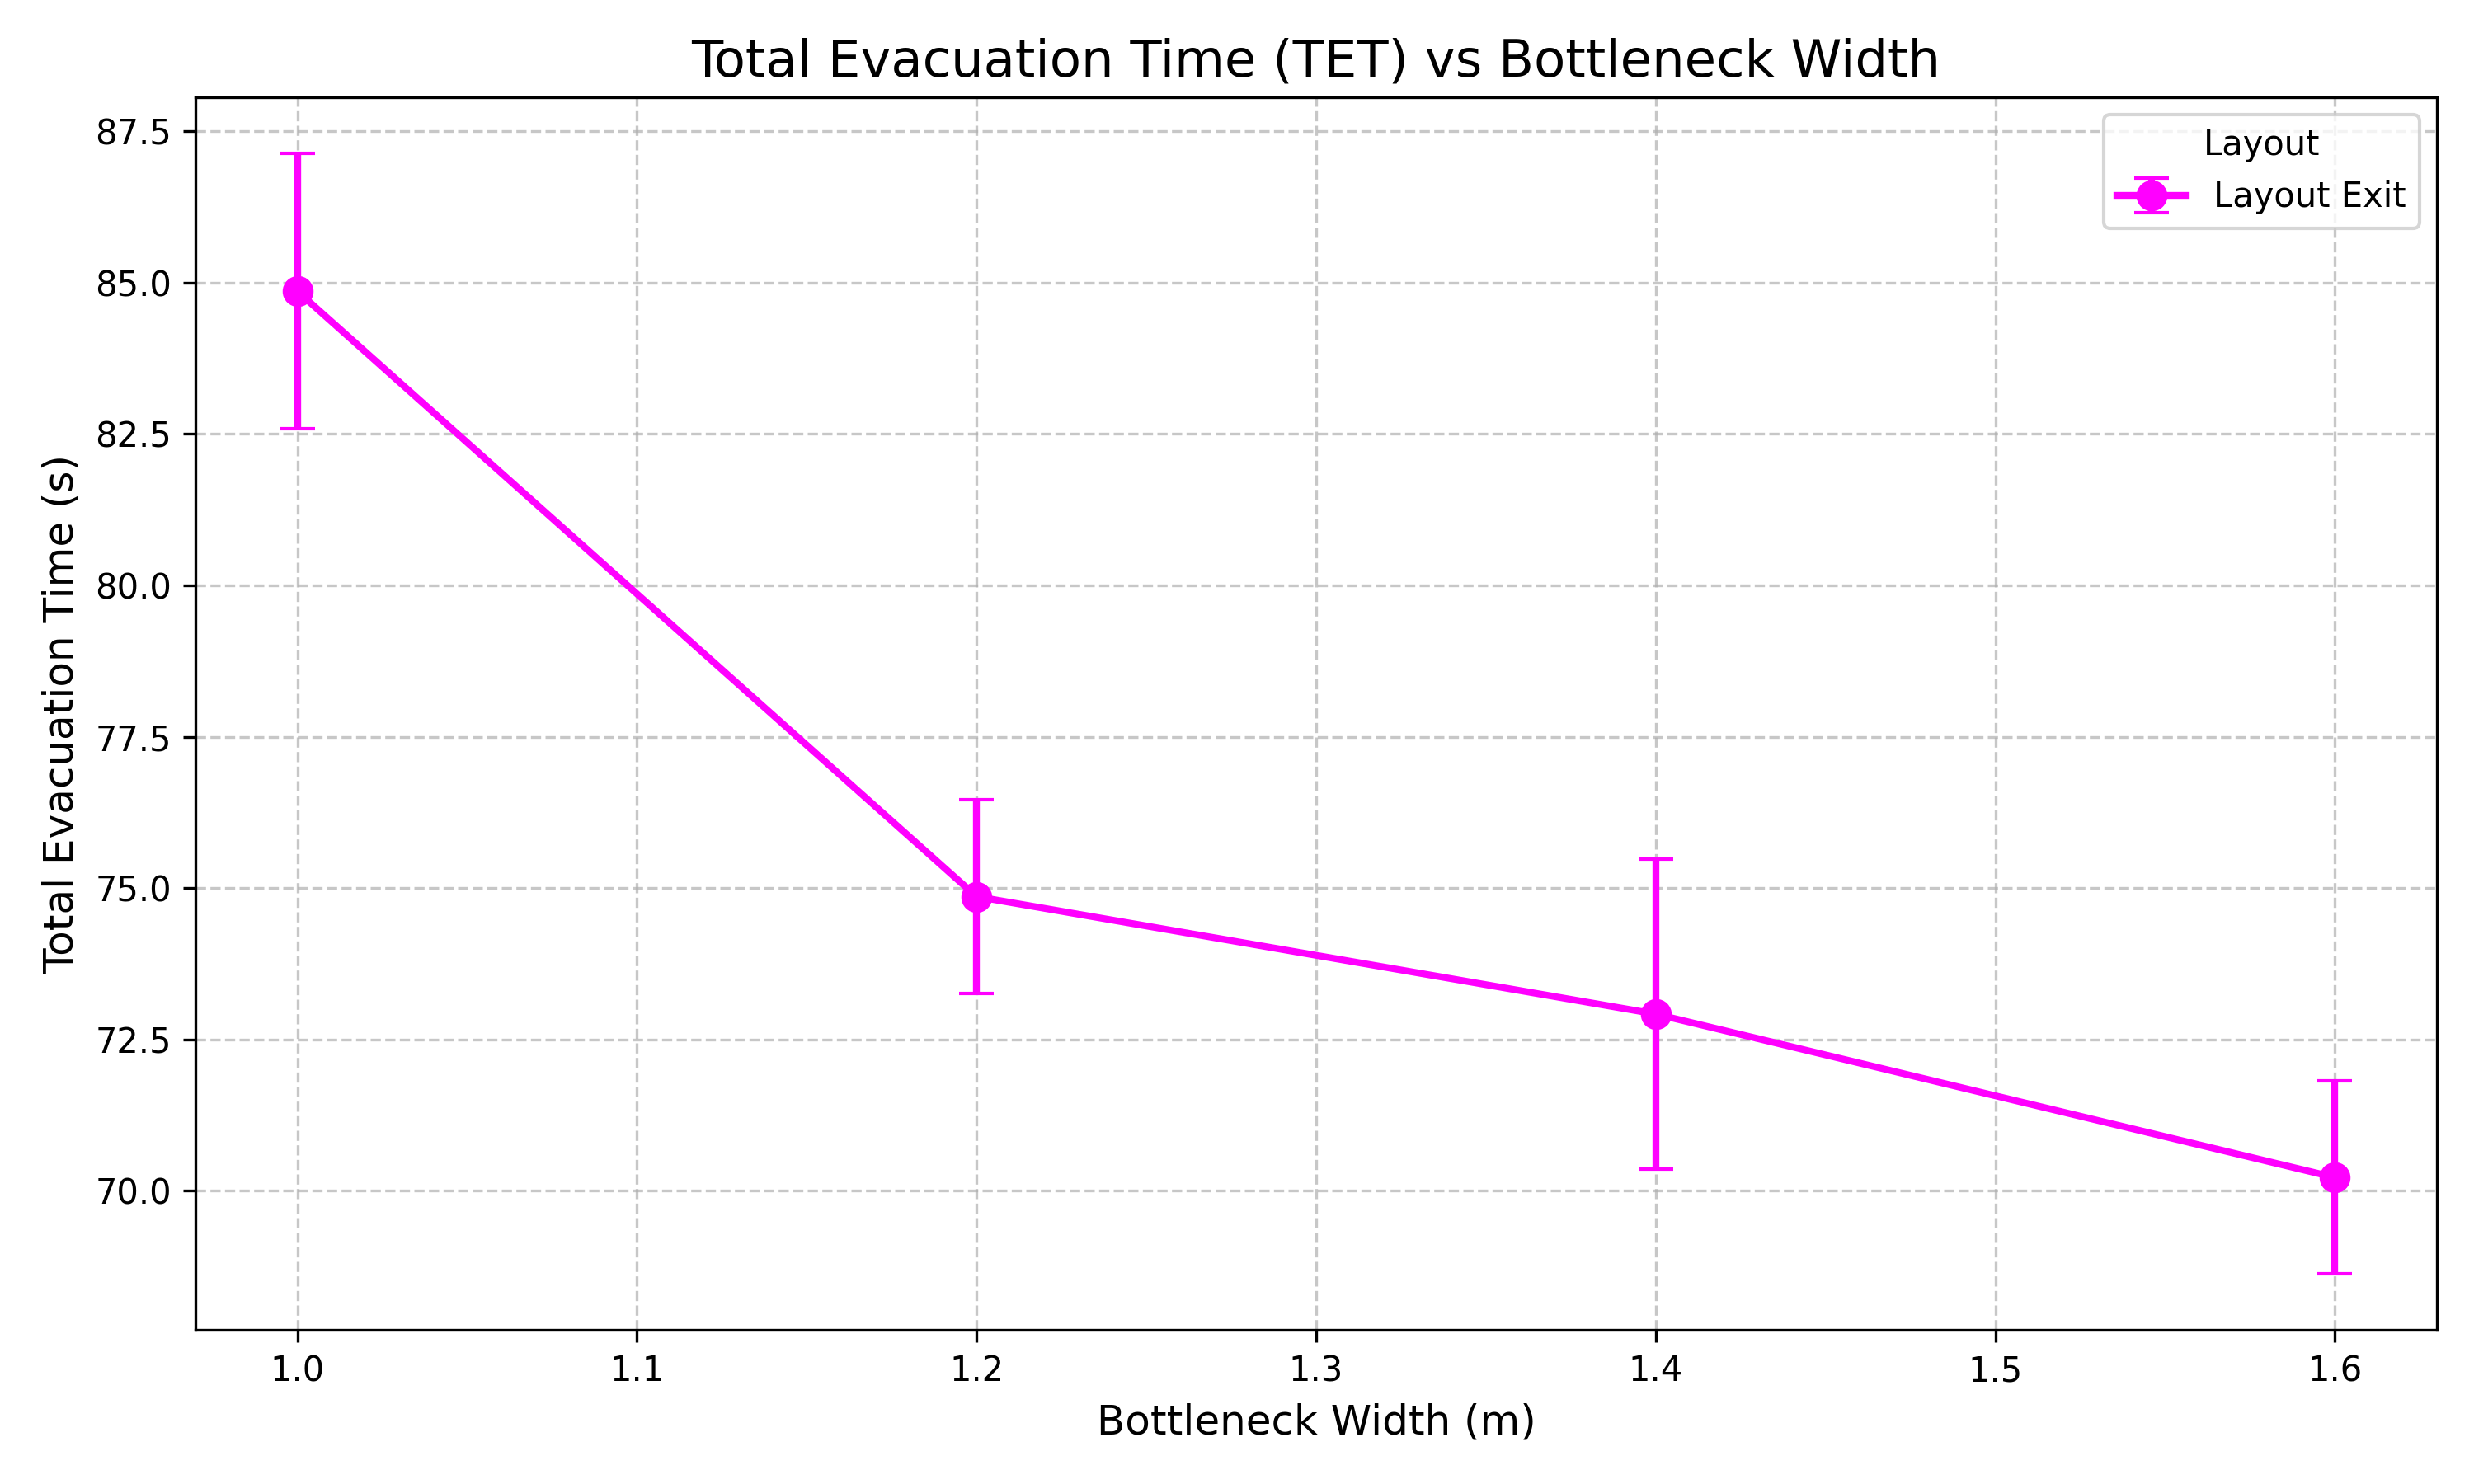
\includegraphics[width=\textwidth]{tet_vs_Bottleneck.png}
    \caption{TET vs Bottleneck Width}
    \label{fig:tet_vs_Bottleneck}
\end{figure}

The speed trajectory diagrams are consistent with the aforementioned trends. At the bottleneck width of 1.0 m \ref{fig:speed_trajectory_layout_1.0m}, the low-speed red zones significantly extend backward, showing queuing phenomena. Due to the queuing phenomenon, agents exhibit obvious convergence behavior at an early stage, beginning to merge lanes with frequent lateral interactions and substantial velocity fluctuations. When the width increases to 1.2 m \ref{fig:speed_trajectory_layout_1.2m}, the low-speed zone noticeably diminishs and becomes concentrated within several meters of the room exits, as well as the merging points be closer to the room exit. The agents' queuing phenomenon visibly disappears during actual simulation observation. On expansion to 1.4 m \ref{fig:speed_trajectory_layout_1.4m} and 1.6 m \ref{fig:speed_trajectory_layout_1.6m} , the low-speed zone continues to diminish and remains close to the doorway, with only brief delays occurring during peak arrival periods, more uniform velocity distribution, and reduced lateral conflicts. The multiple simulations show that the main corridor and overall paths leading to each exit remain consistent, while width variations not triggering large-scale route diversions. The most significant differences are concentrated in the flow microstructure within the final several meters of the exit area.
\begin{figure}[h]
    \centering
    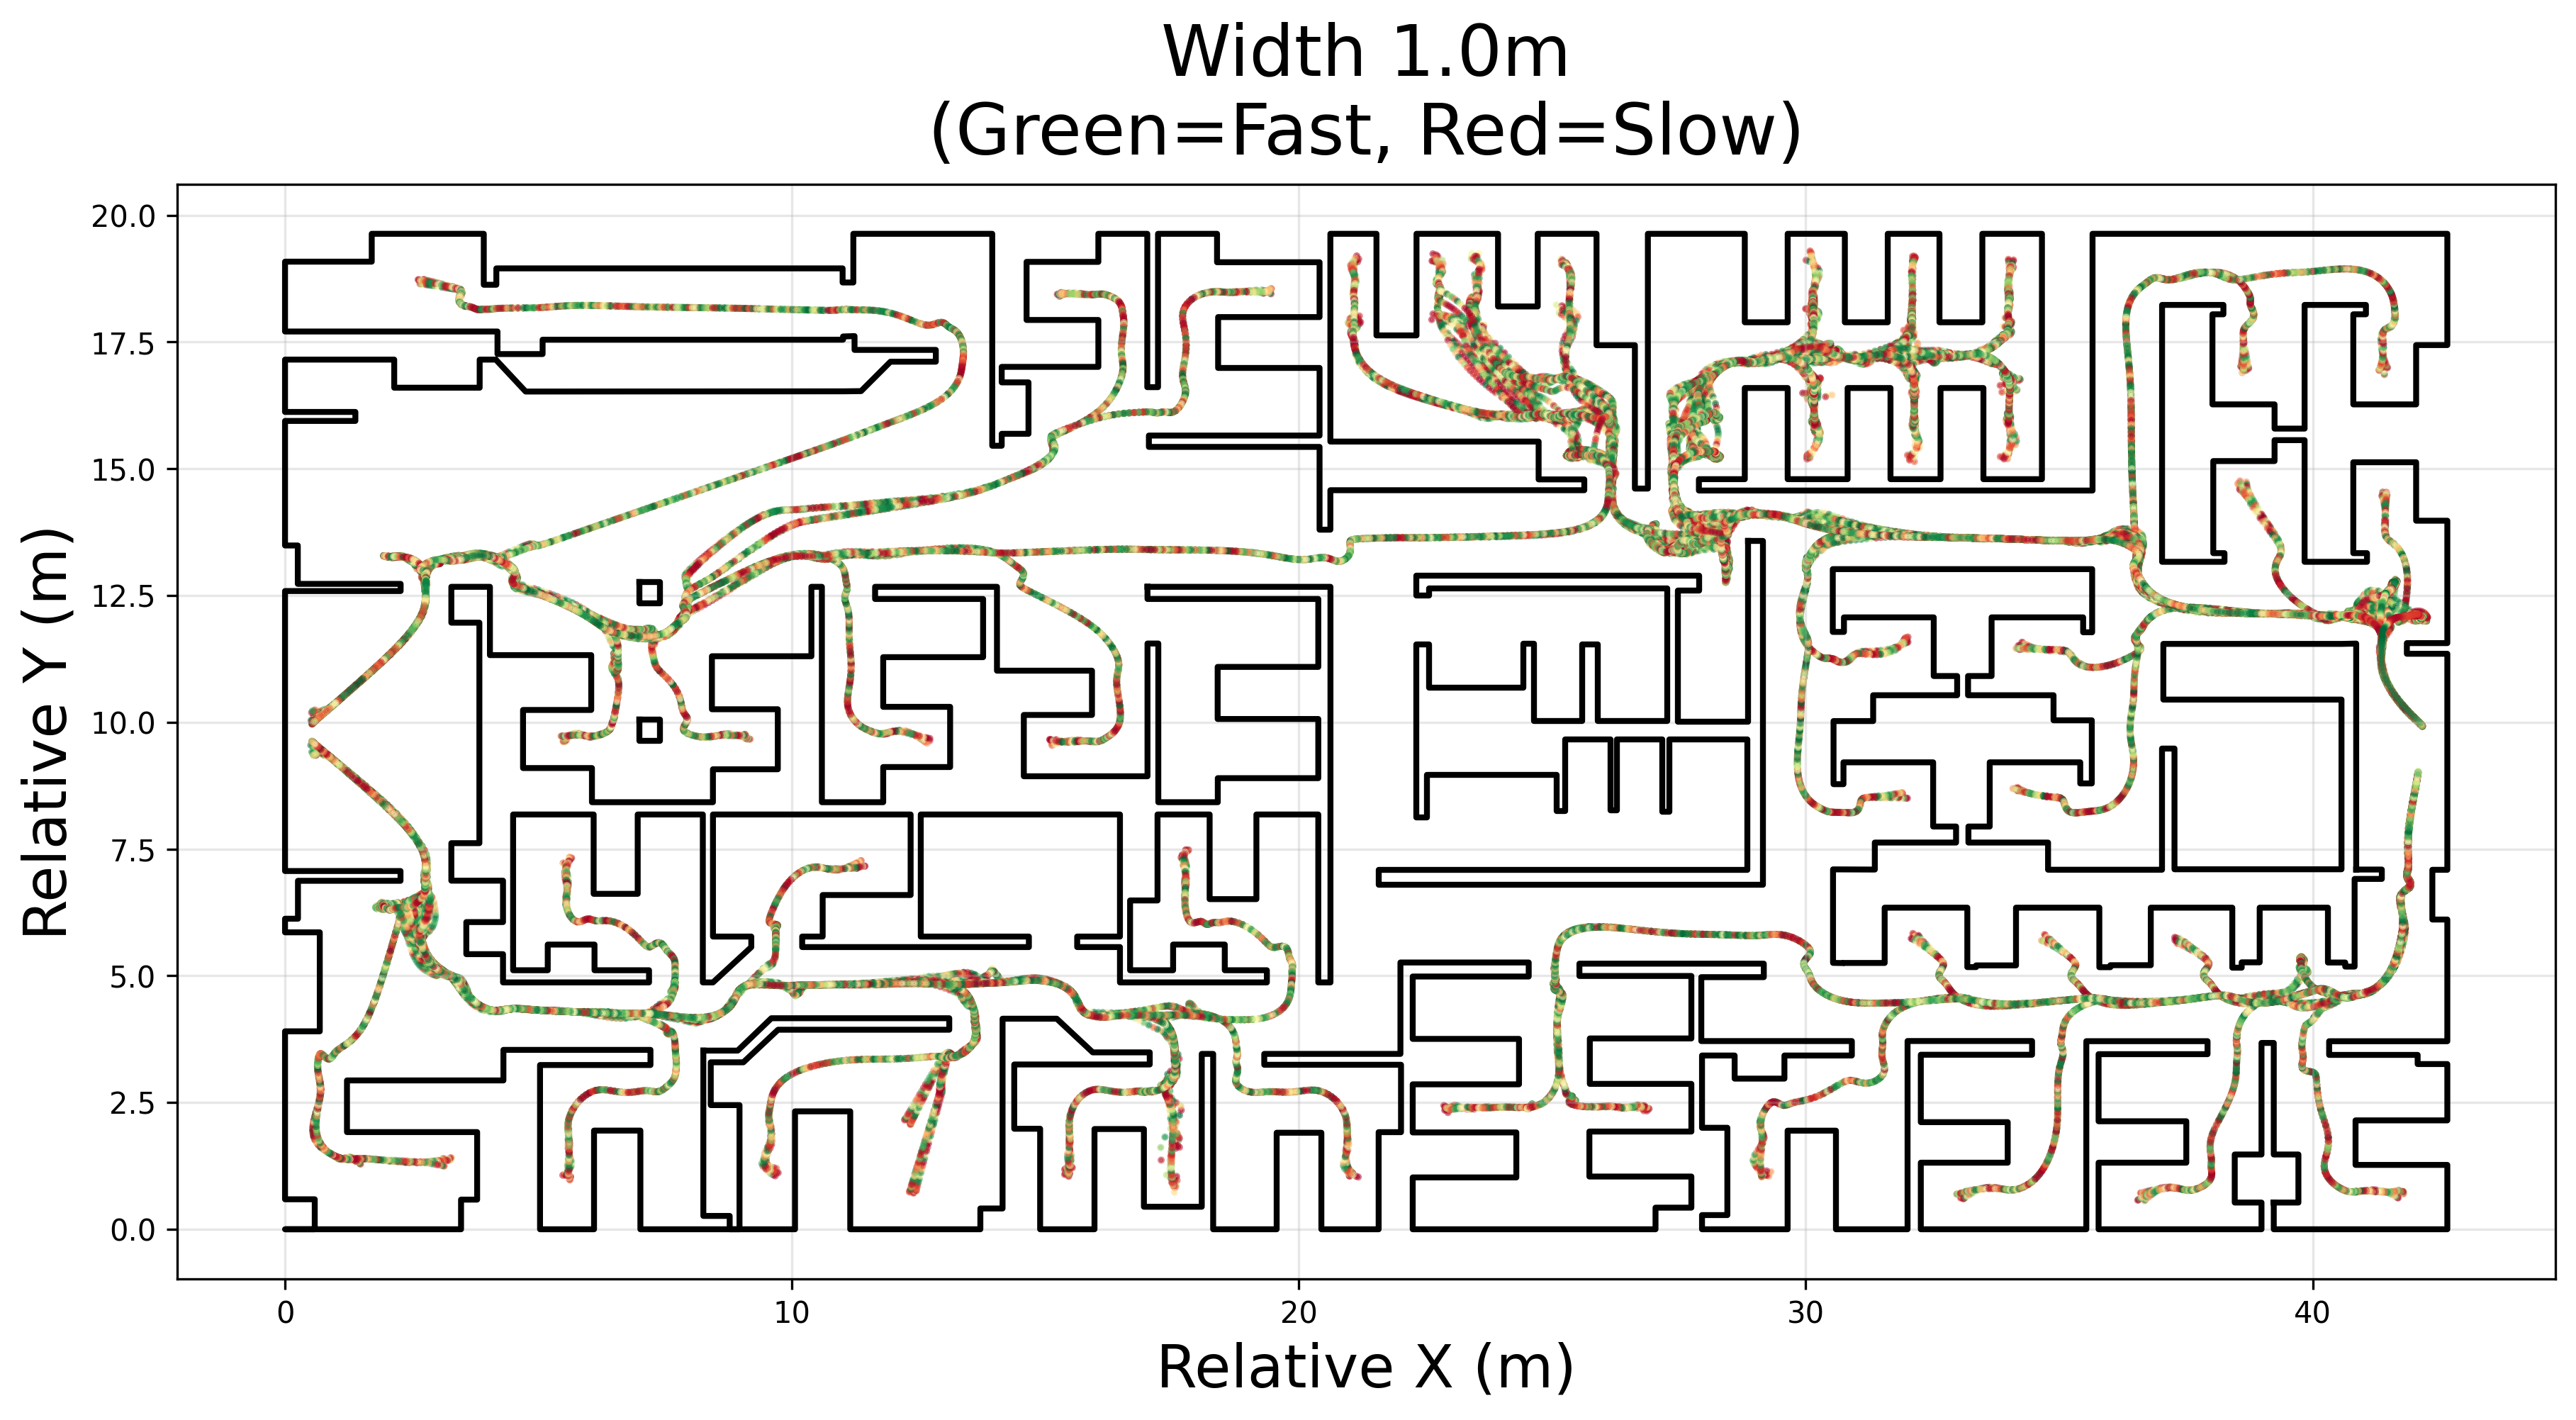
\includegraphics[width=\textwidth]{speed_trajectory_Exit_width_1.0m.png}
    \caption{Speed and Trajectories for 1.0m Bottleneck Width}
    \label{fig:speed_trajectory_layout_1.0m}
\end{figure}
\begin{figure}[h]
    \centering
    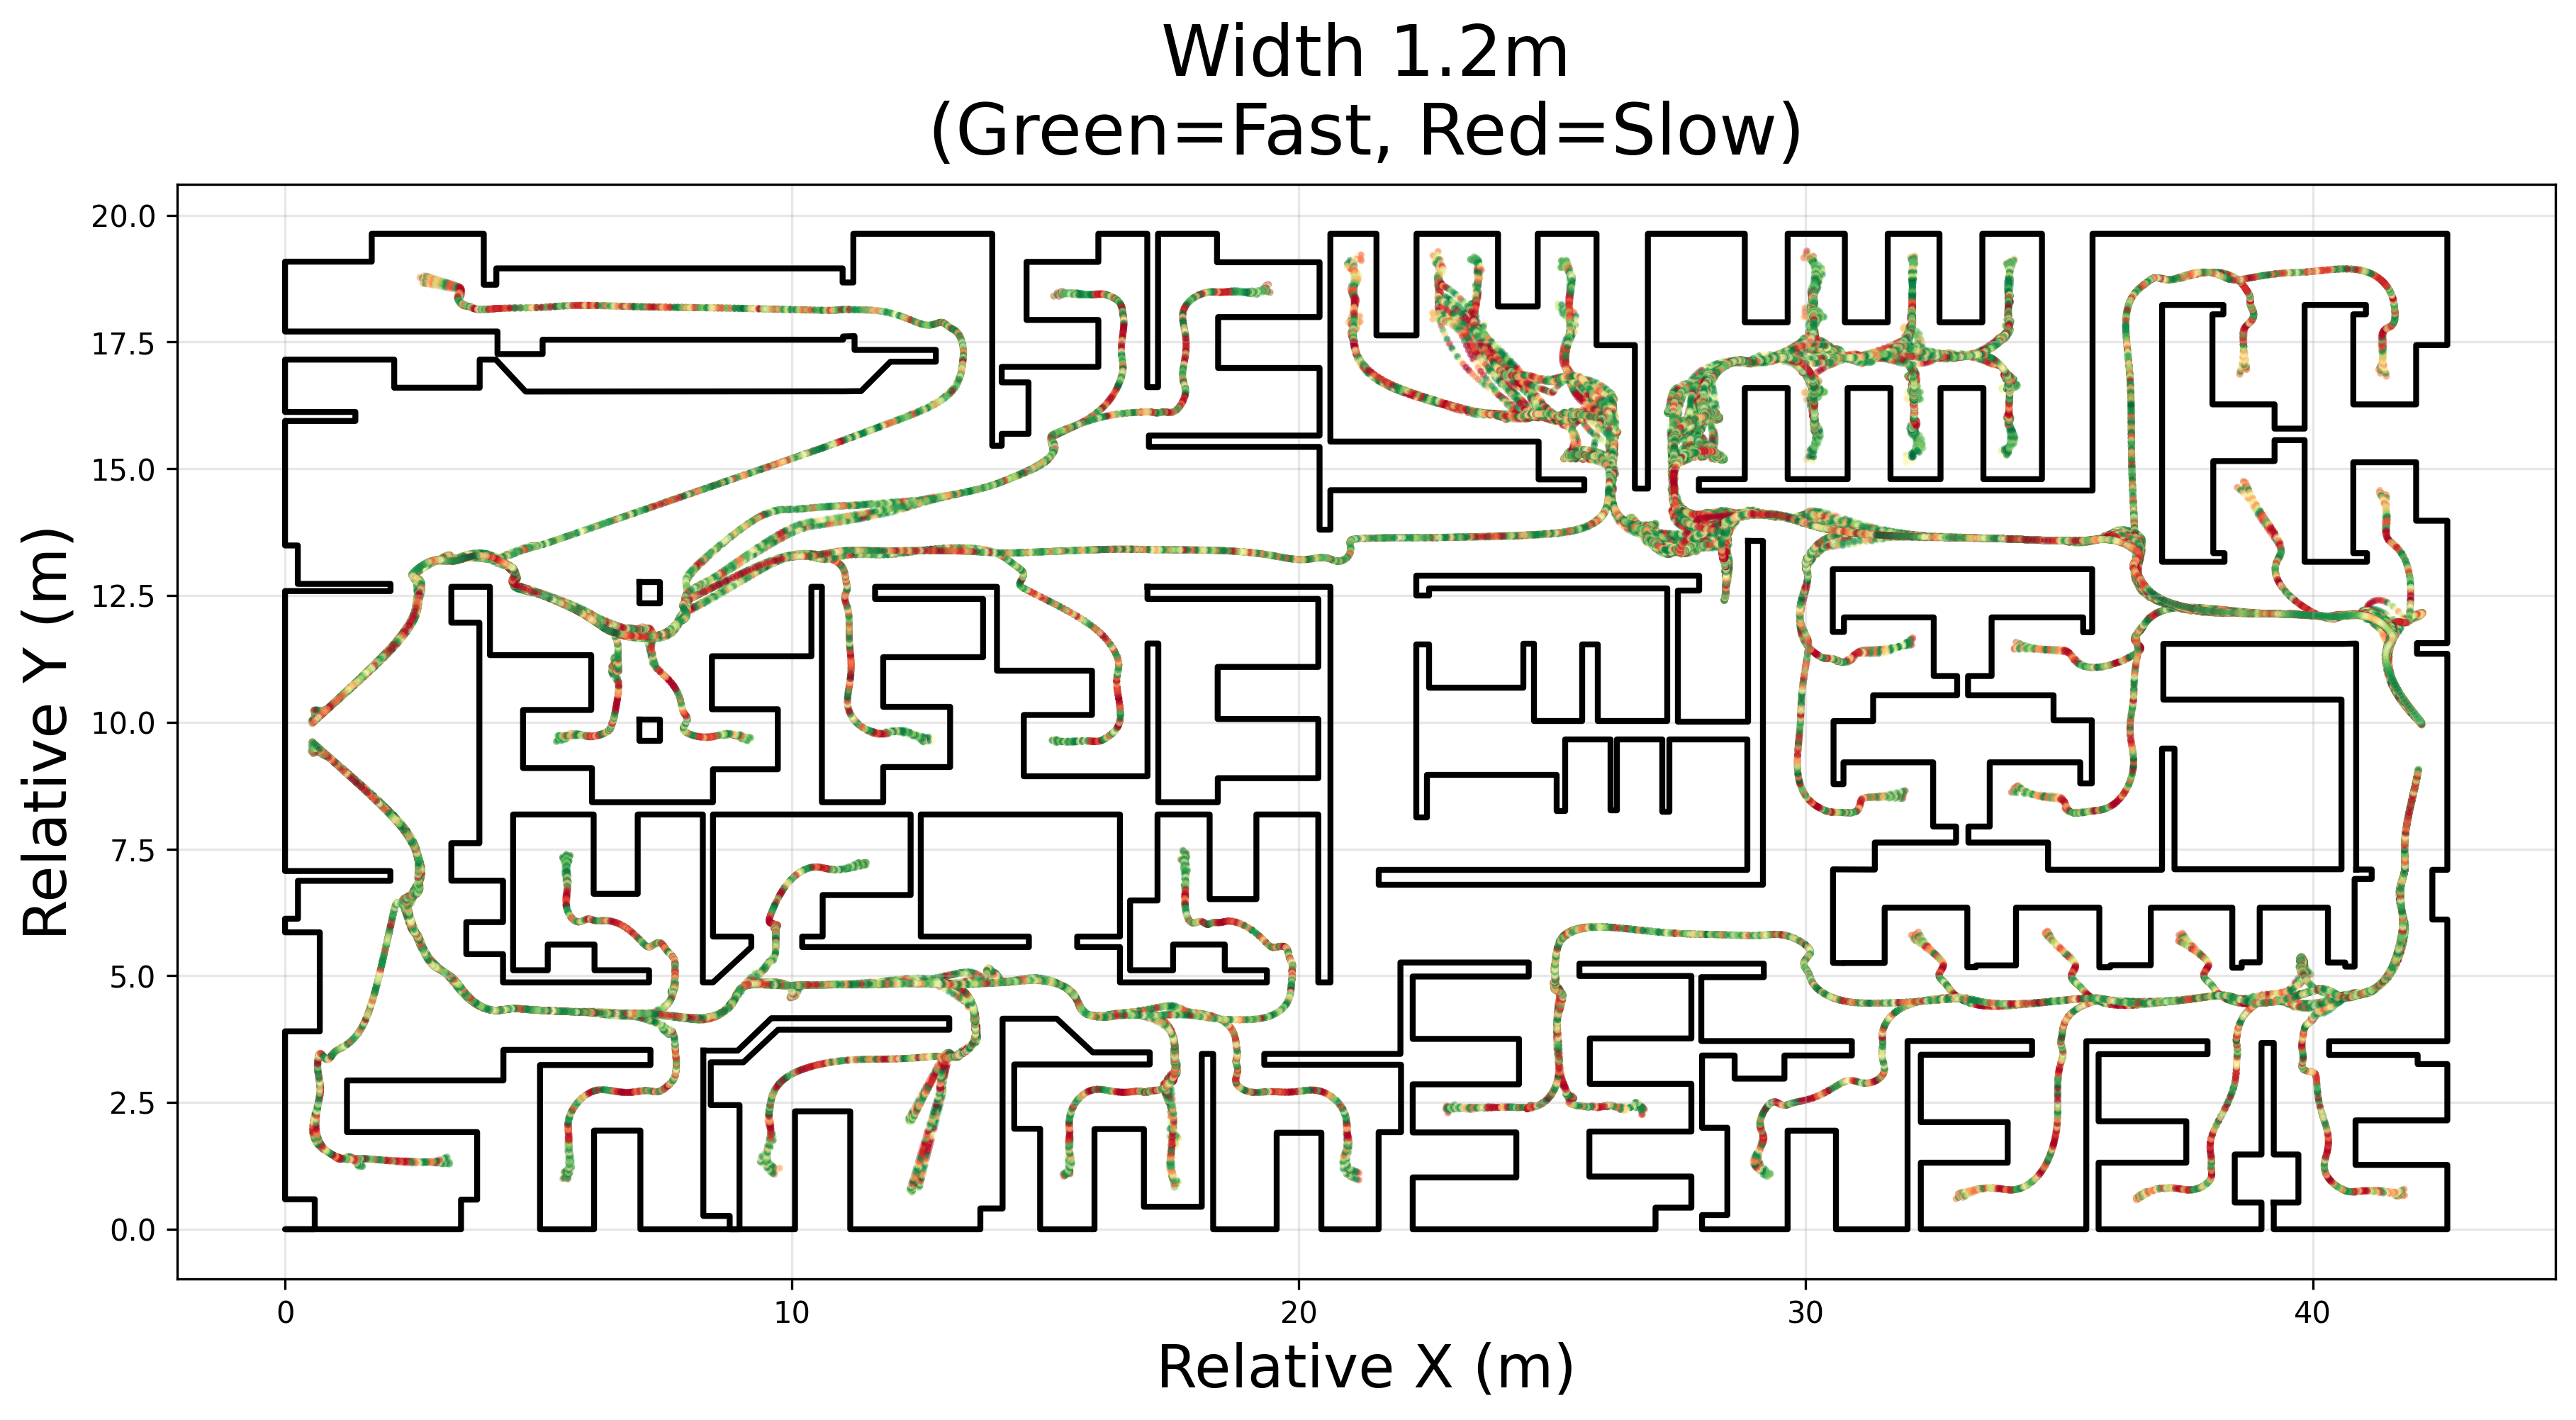
\includegraphics[width=\textwidth]{speed_trajectory_Exit_width_1.2m.png}
    \caption{Speed and Trajectories for 1.2m Bottleneck Width}
    \label{fig:speed_trajectory_layout_1.2m}
\end{figure}
\begin{figure}[h]
    \centering
    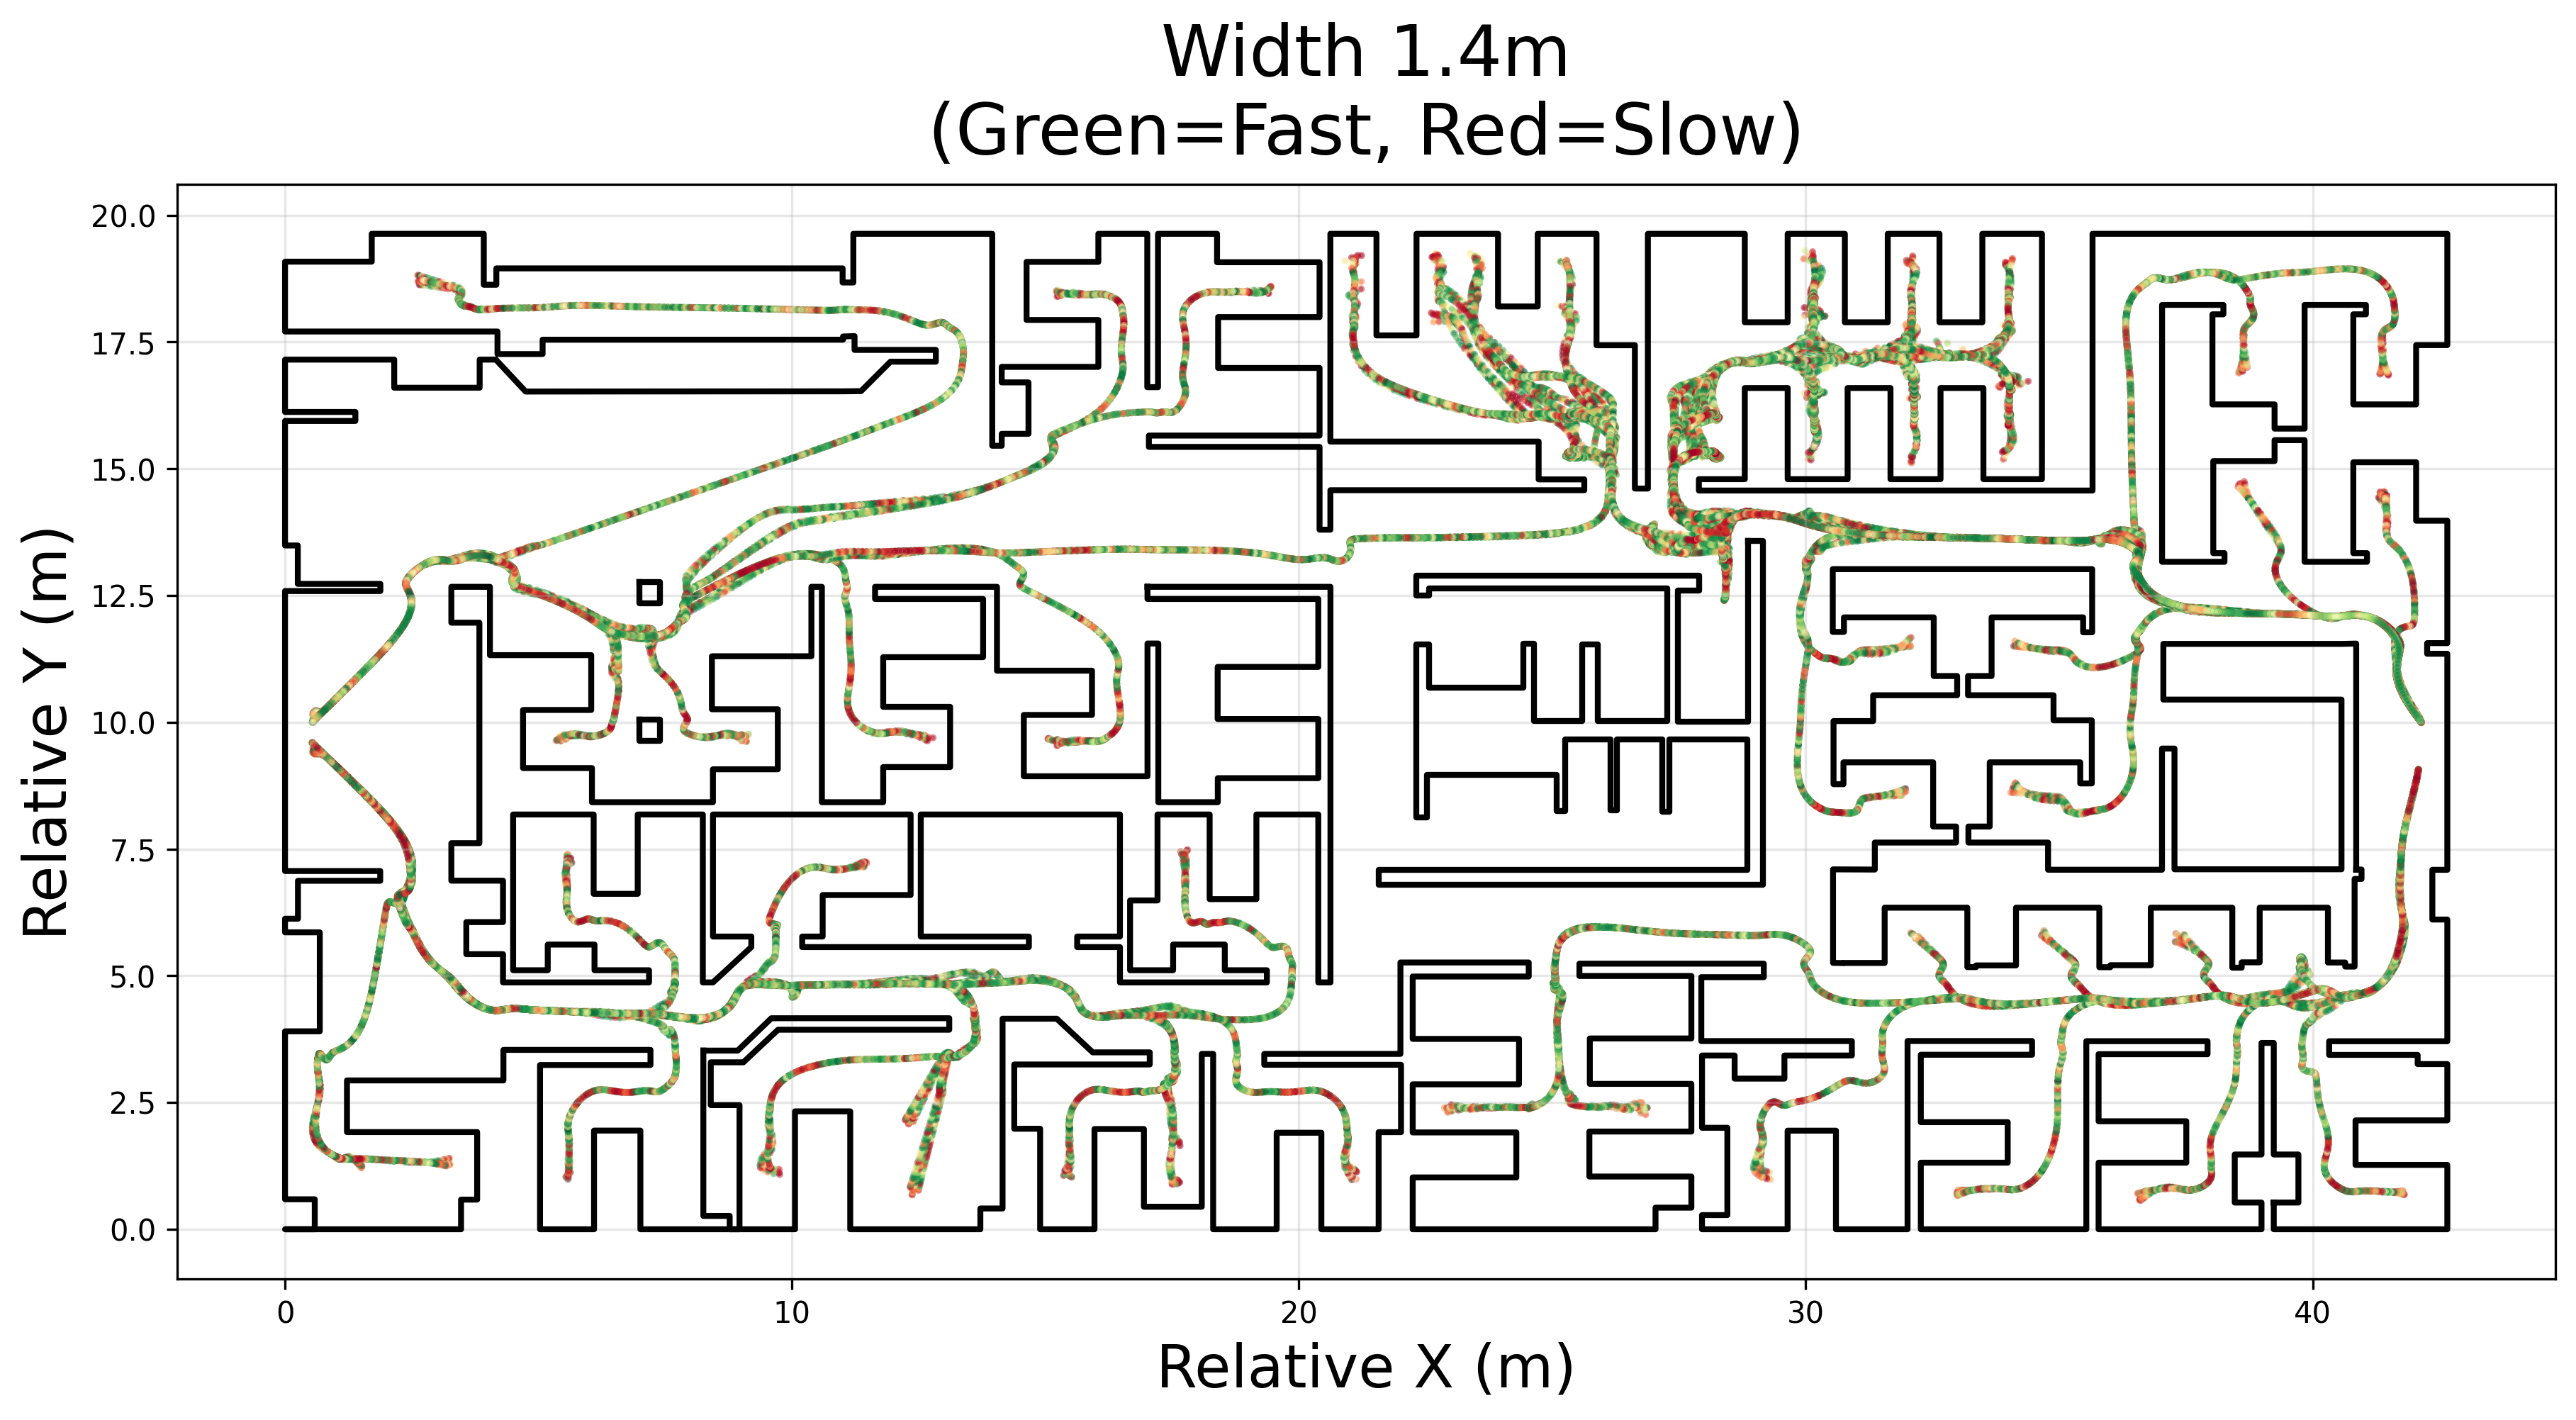
\includegraphics[width=\textwidth]{speed_trajectory_Exit_width_1.4m.png}
    \caption{Speed and Trajectories for 1.4m Bottleneck Width}
    \label{fig:speed_trajectory_layout_1.4m}
\end{figure}
\begin{figure}[h]
    \centering
    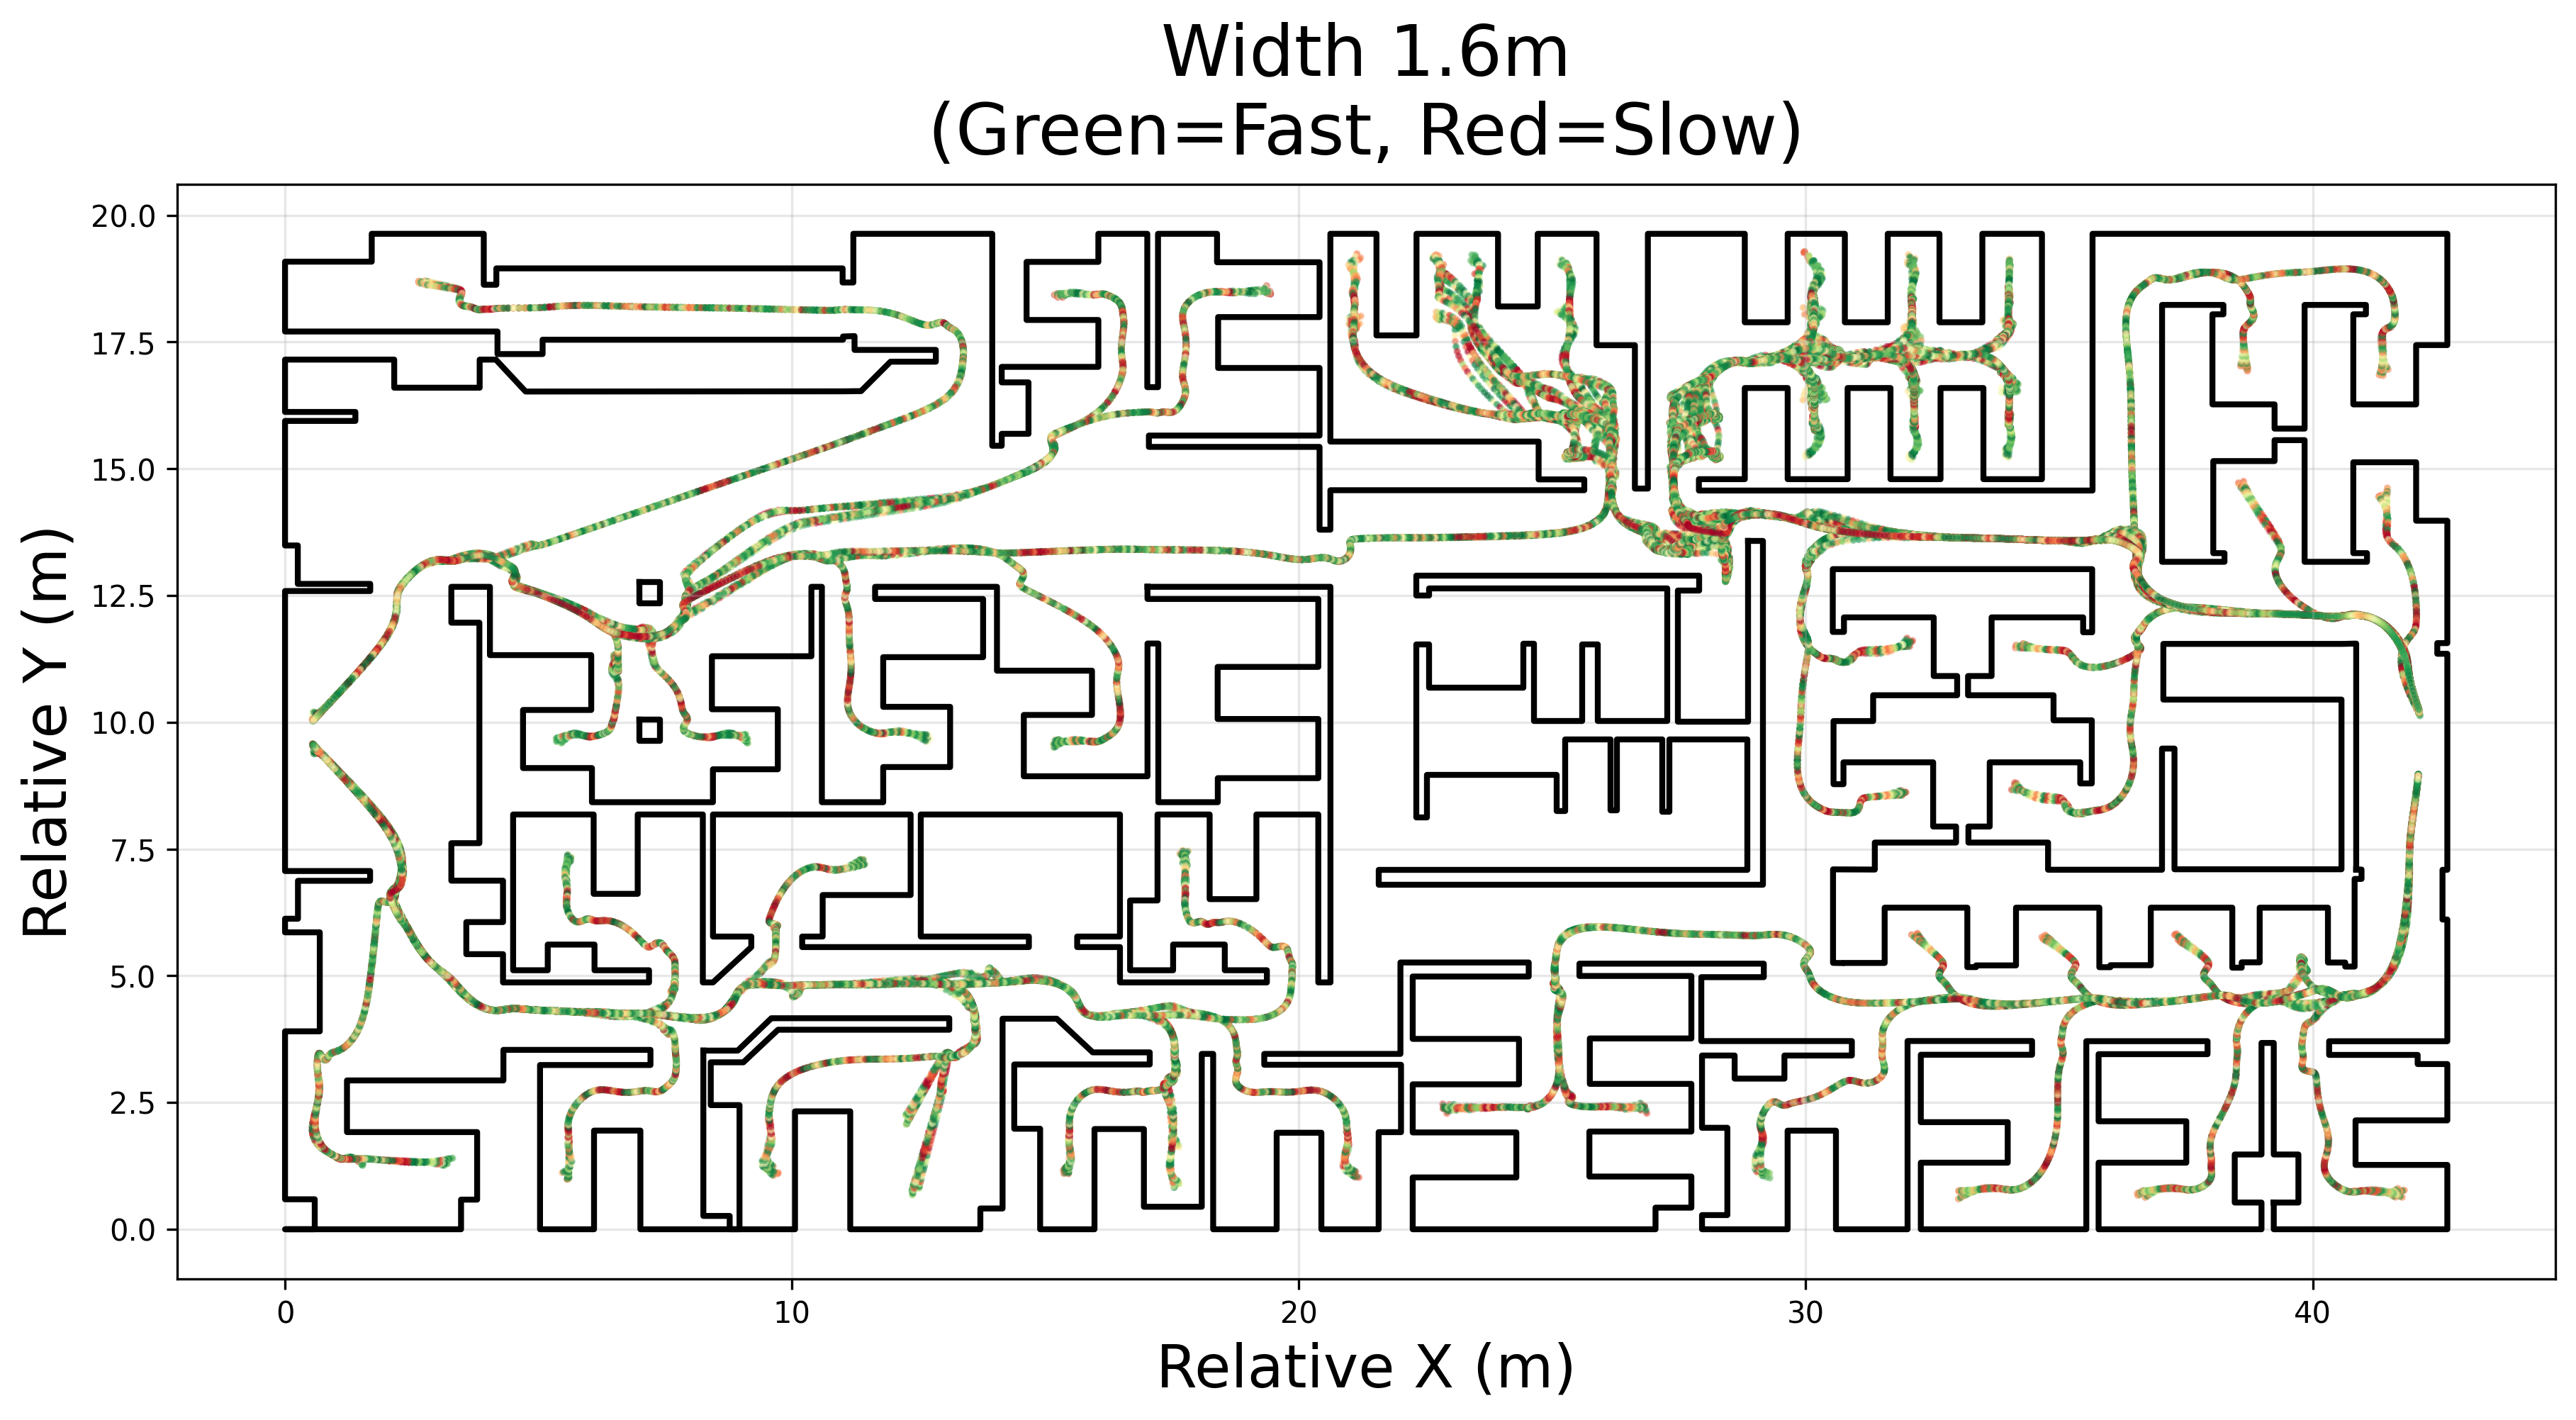
\includegraphics[width=\textwidth]{speed_trajectory_Exit_width_1.6m.png}
    \caption{Speed and Trajectories for 1.6m Bottleneck Width}
    \label{fig:speed_trajectory_layout_1.6m}
\end{figure}

The overlapping trajectories illustrate that the main path remains relatively stable across all widths, with only slight differences showed up in the congestion before the exit. Corresponding to the performance of TET error bars, the run results under wider gate conditions are more concentrated, indicating that intermittent congestion in the exit vicinity is weakened, system behavior becomes more predictable, and the consistency of repeated experiments is also improved.

Based on the comprehensive evidence from both TET curves and velocity trajectory analysis, the main conclusions can be summarized in the following narrative. The most significant performance improvement occurred when increasing the bottleneck width from 1.0 m to 1.2 m, during which the queuing phenomenom disppeared, and the merging points approached the exit. Further widening to 1.4 m and 1.6 m continued to reduce TET, but with smaller improvements, mainly manifesting as further reduction of short-term low-speed conditions near the exit line.  These results provide direct support for subsequent design recommendations, with specific conclusions and suggestions to be presented in the Conclusion section.

\subsection{Coupling Effect of Corridor Entrance and Passage Gate Width}
Based on the experiments described in the last section, we selected 1.2m under simulated stable conditions as the standard bottleneck width parameter to test the coupling effect of room door width and corridor gate width, in order to minimize the conflicts and interference caused by bottlenecks as much as possible, thereby improving the system's robustness and accuracy.

According to the heat maps \ref{fig:tet_vs_room_corridor_coupling}, The horizontal axis represents corridor gate width, and the vertical axis represents room door width, with both parameters taking values of 1.0, 1.2, 1.4, and 1.6 m. For each combination, multiple independent simulations were conducted while maintaining agents numbers, layout, and model parameters. The mean and standard deviation of total evacuation time(TET) were calculated and presented as the color variation.

Among all combinations, the shortest TET was 69.7 s, which occurs when corridor width is 1.4m and room door width is 1.2m. The longest TET was 89.5 s, showing when corridor width is 1.0m and room door width is 1.4m. When corridor gate width increased to 1.4 m and above, the TET for all combinations clearly converged to approximately 70-72 s, with standard deviations generally decreasing to about 1-2 s, indicating that the system is getting stable. Especially significant is that when the corridor gates were narrow (1.0 or 1.2 m), increasing room door width alone significantly slowed evacuation time. This phenomenon is consistent with merging conflicts and queue backtracking observed in speed-trajectory diagrams, and this mechanism will be further explained in conjunction with speed-trajectory diagrams in subsequent paragraphs.
\begin{figure}[h]
    \centering
    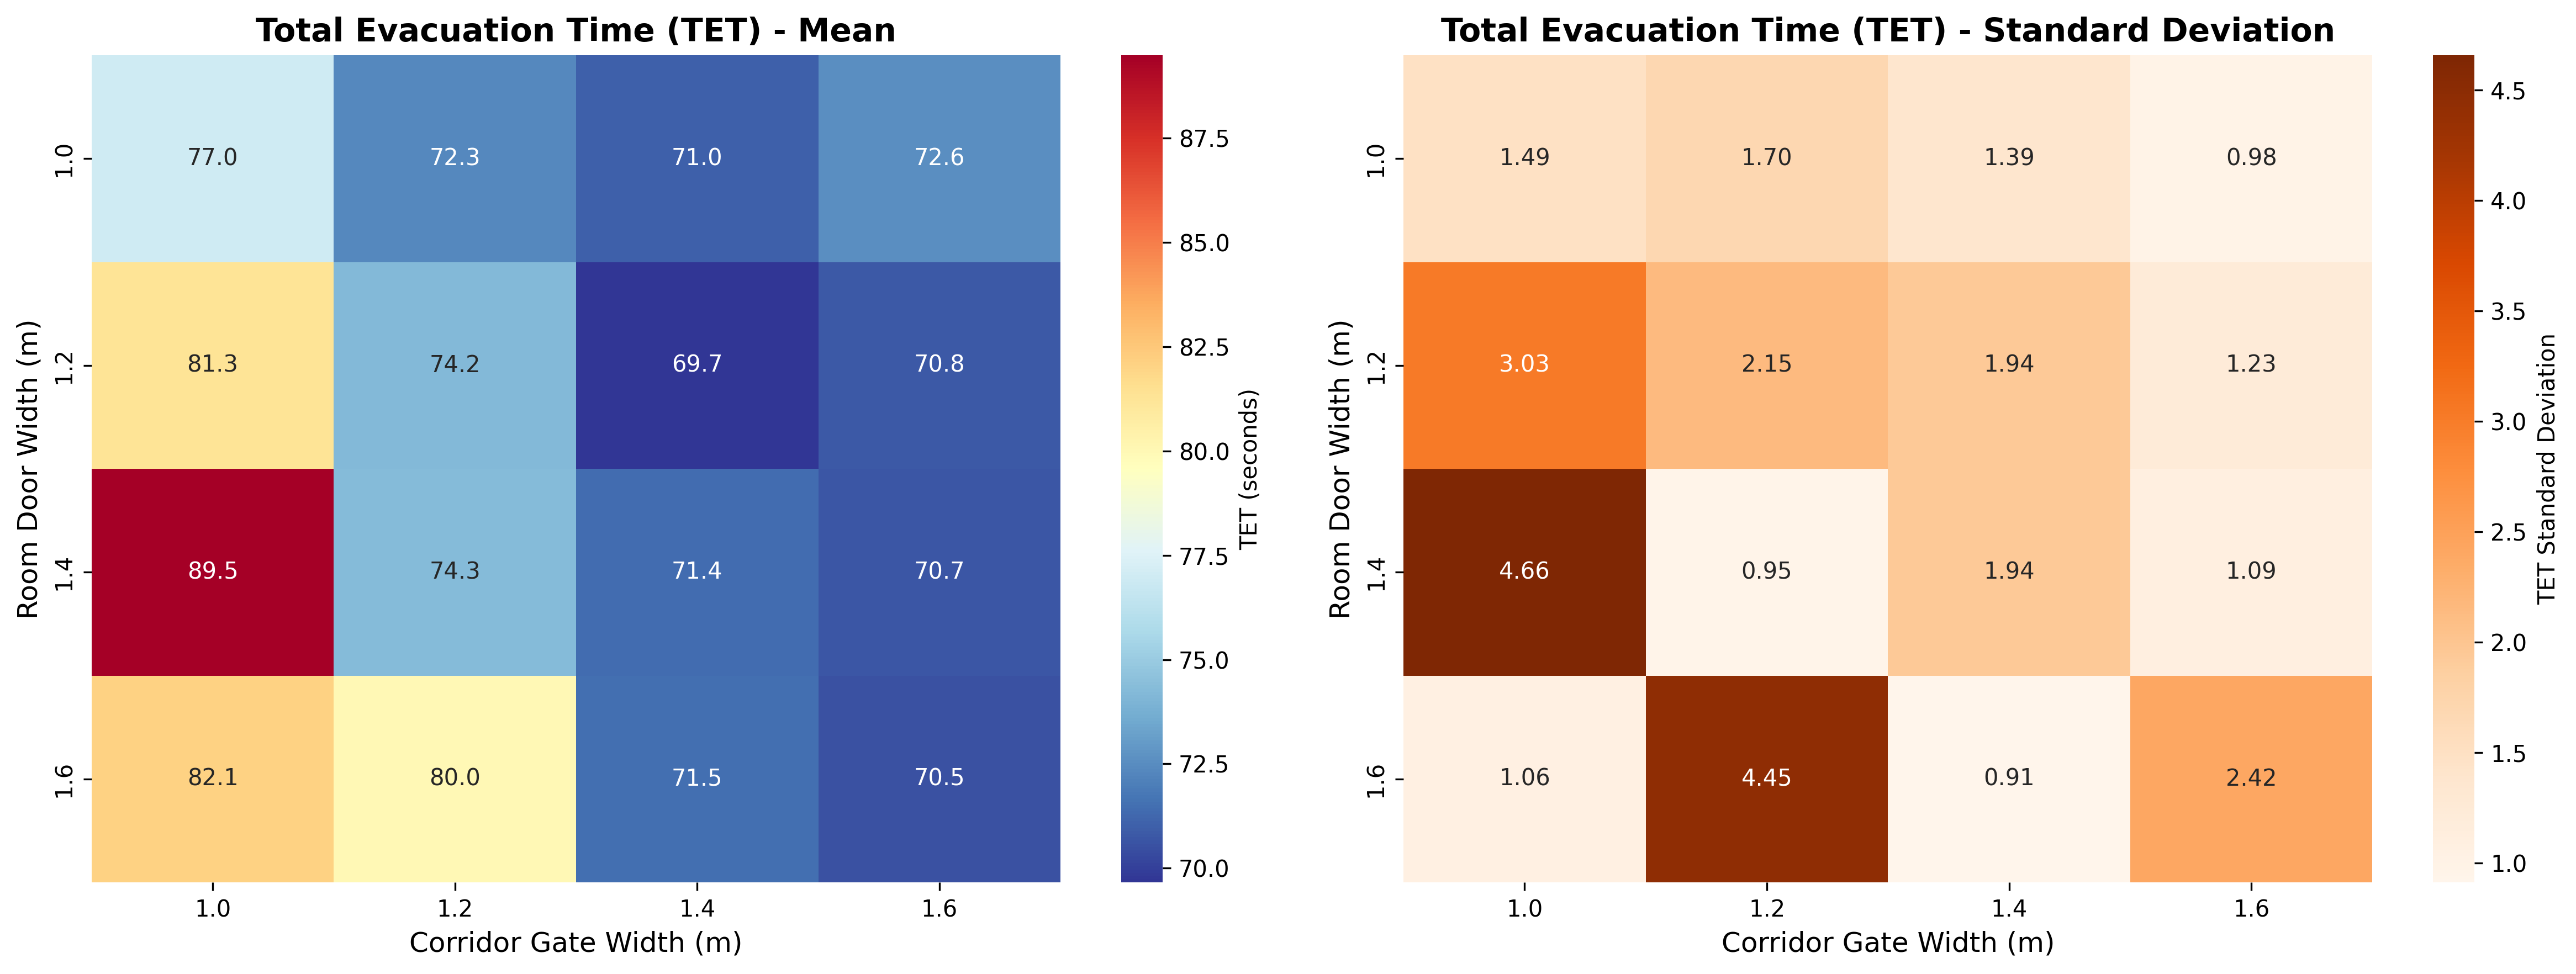
\includegraphics[width=\textwidth]{tet_seaborn_heatmap_multiroom.png}
    \caption{TET vs Room-Corridor Coupling}
    \label{fig:tet_vs_room_corridor_coupling}
\end{figure}

\begin{figure} [H]
    \centering
    \begin{subfigure}[b]{.45\linewidth}
        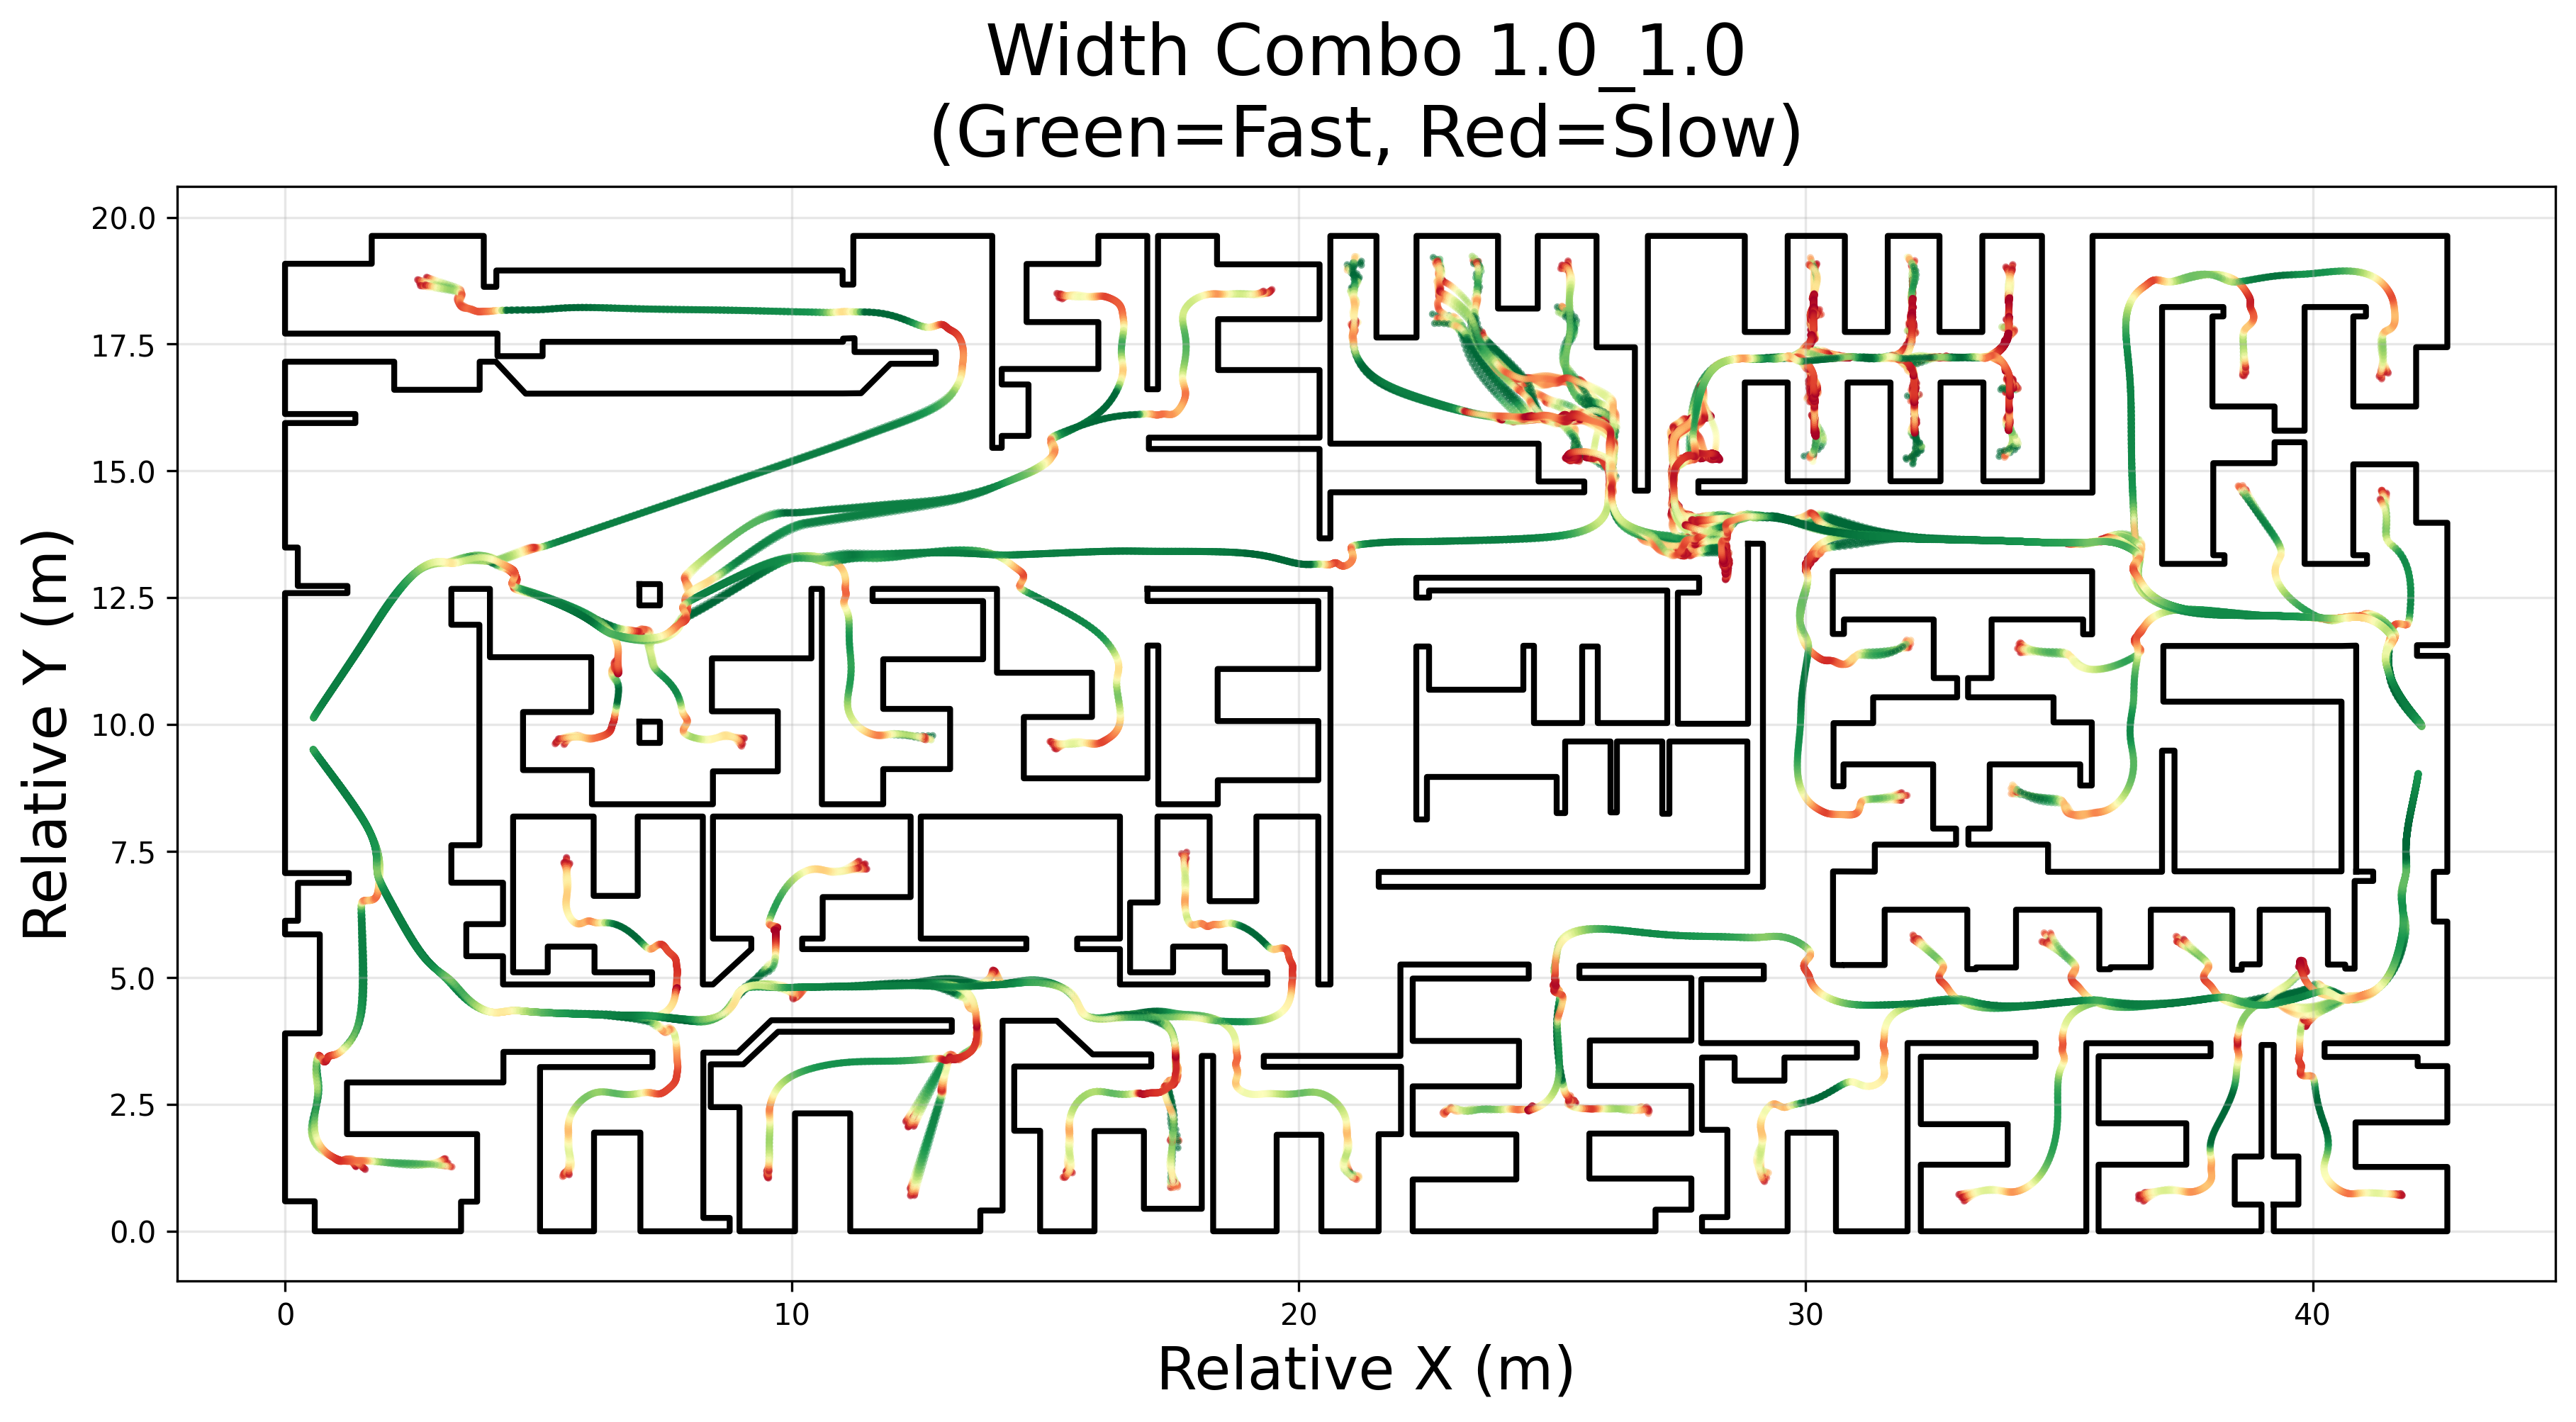
\includegraphics[width=\linewidth]
        {speed_trajectory_MultiRoom_width_1.0_1.0.png}
        \caption{Width Combo 1.0m and 1.0m}
        \label{fig:width_combo_1.0_1.0m}
    \end{subfigure}
    \begin{subfigure}[b]{.45\linewidth}
        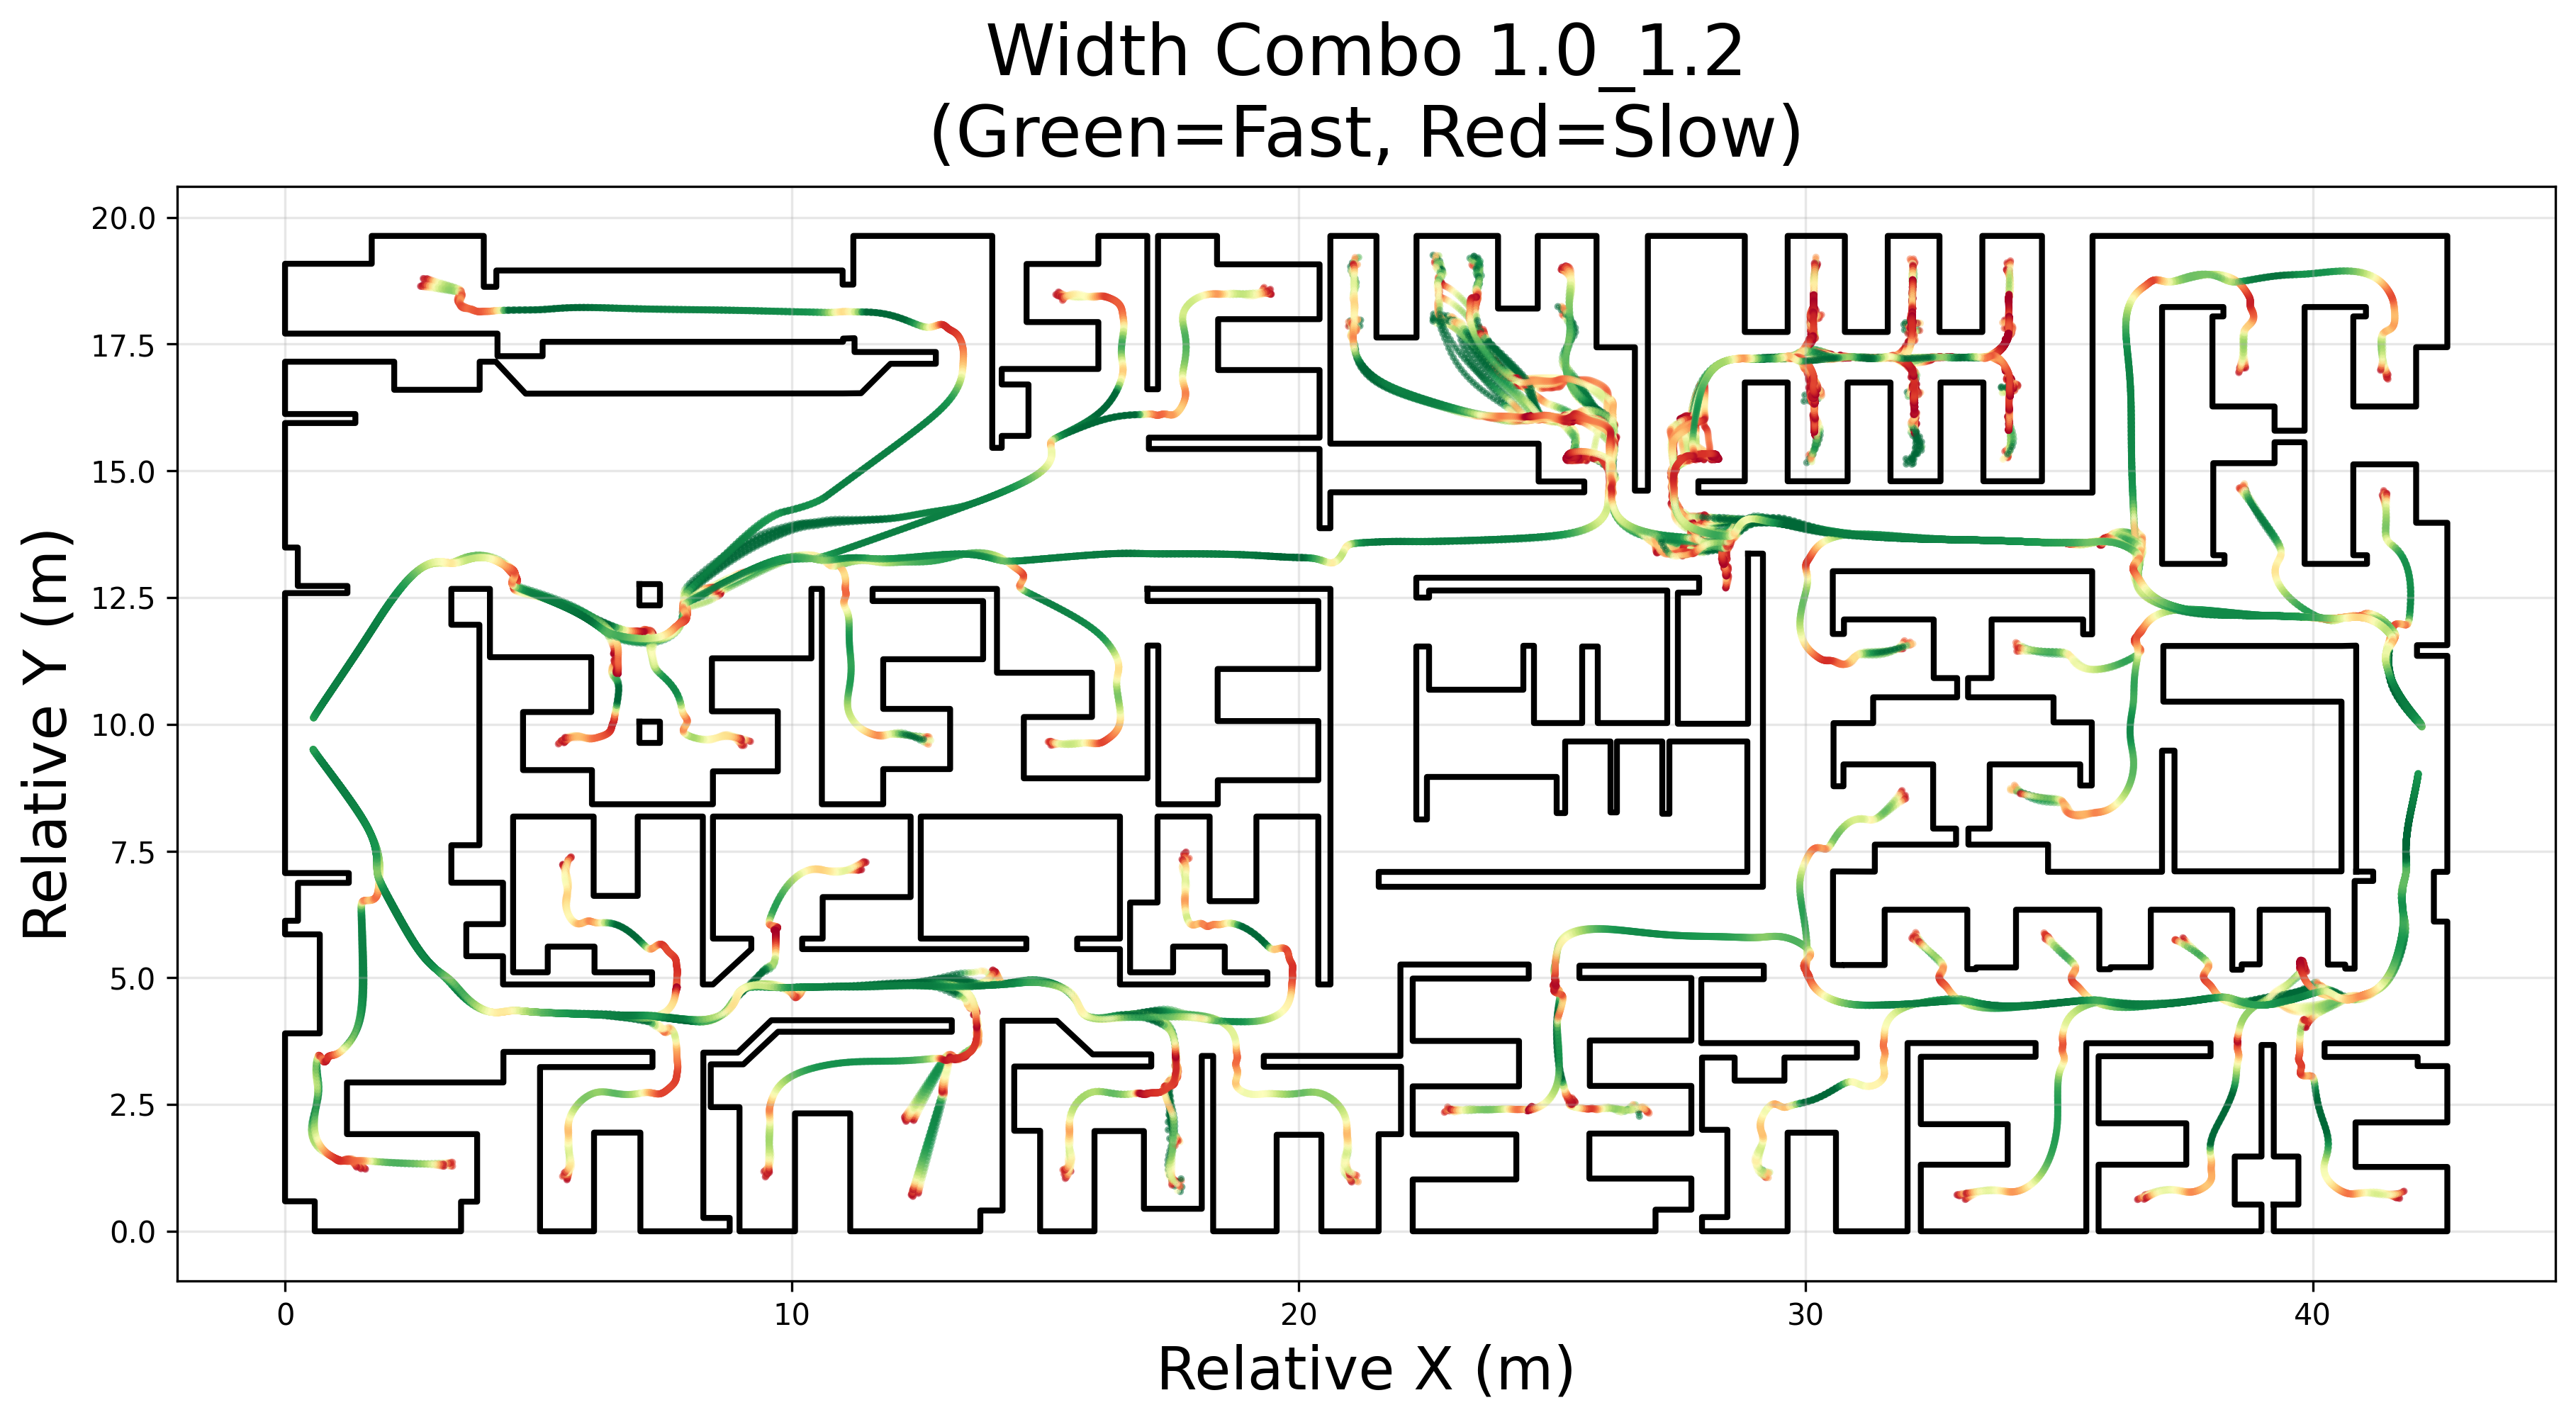
\includegraphics[width=\linewidth]{
            speed_trajectory_MultiRoom_width_1.0_1.2.png}
        \caption{Width Combo 1.0m and 1.2m}
        \label{fig:width_combo_1.0_1.2m}
    \end{subfigure}
    \begin{subfigure}[b]{.45\linewidth}
        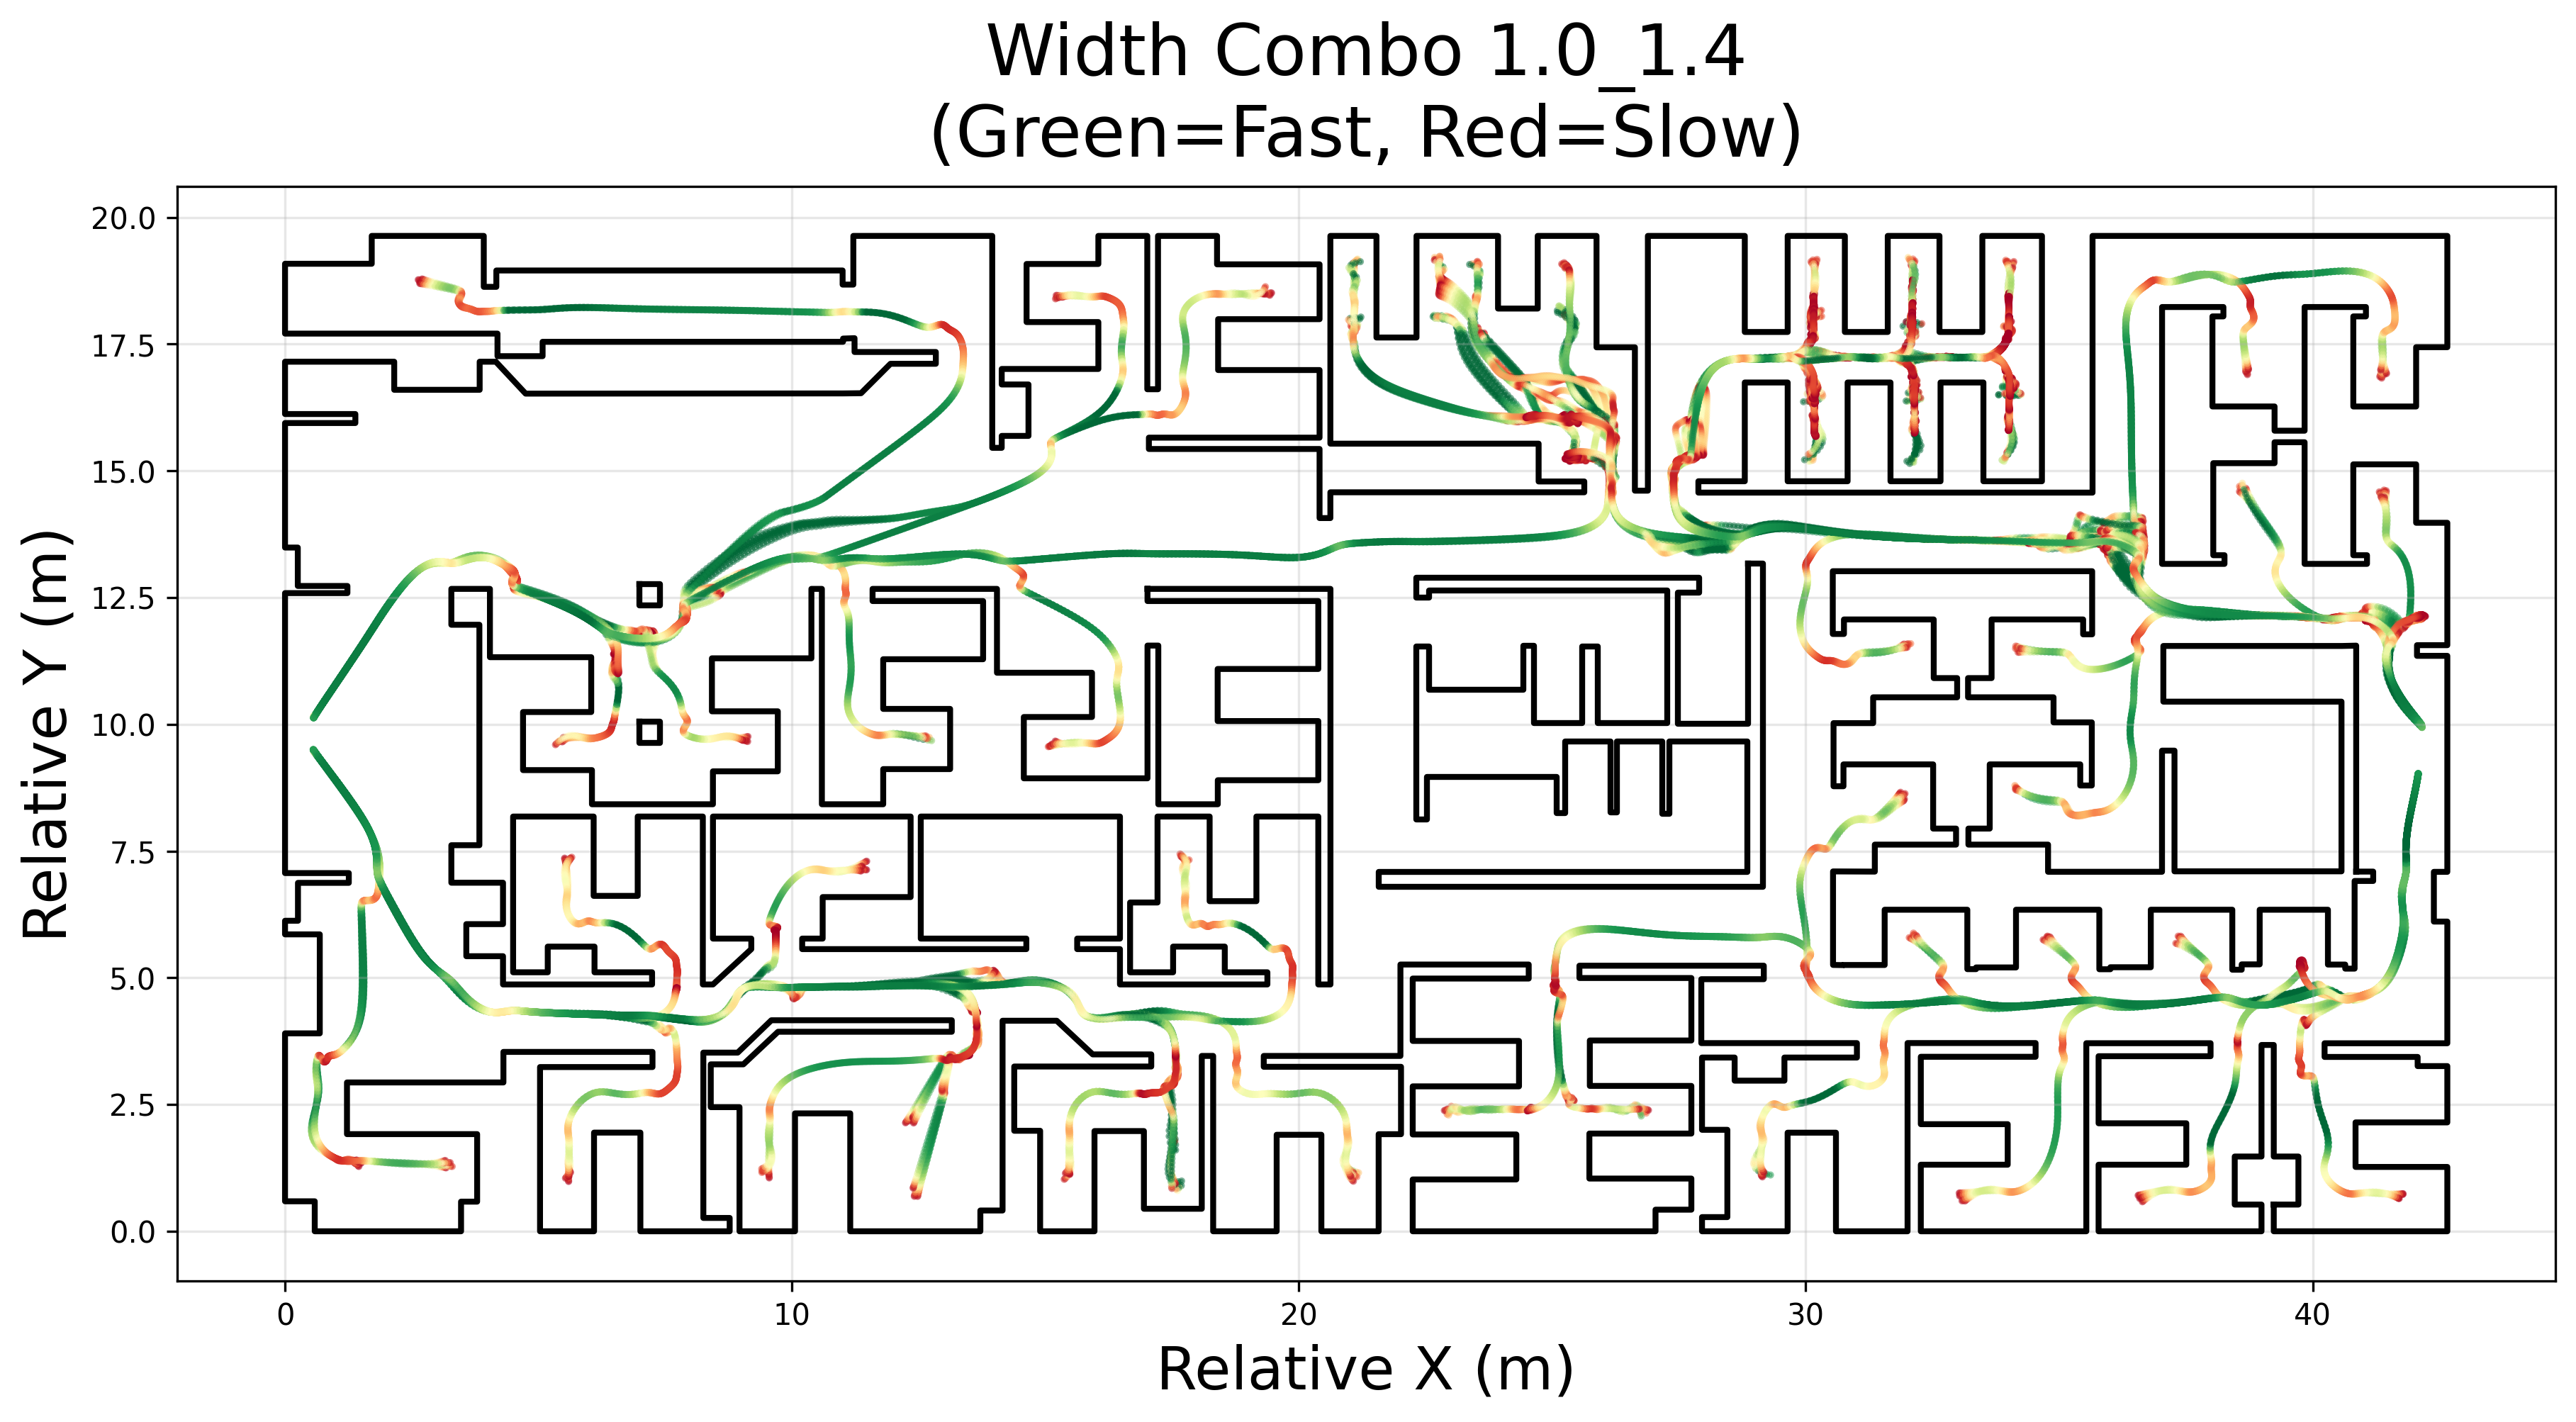
\includegraphics[width=\linewidth]{
            speed_trajectory_MultiRoom_width_1.0_1.4.png}
        \caption{Width Combo 1.0m and 1.4m}
        \label{fig:width_combo_1.0_1.4m}
    \end{subfigure}
    \begin{subfigure}[b]{.45\linewidth}
        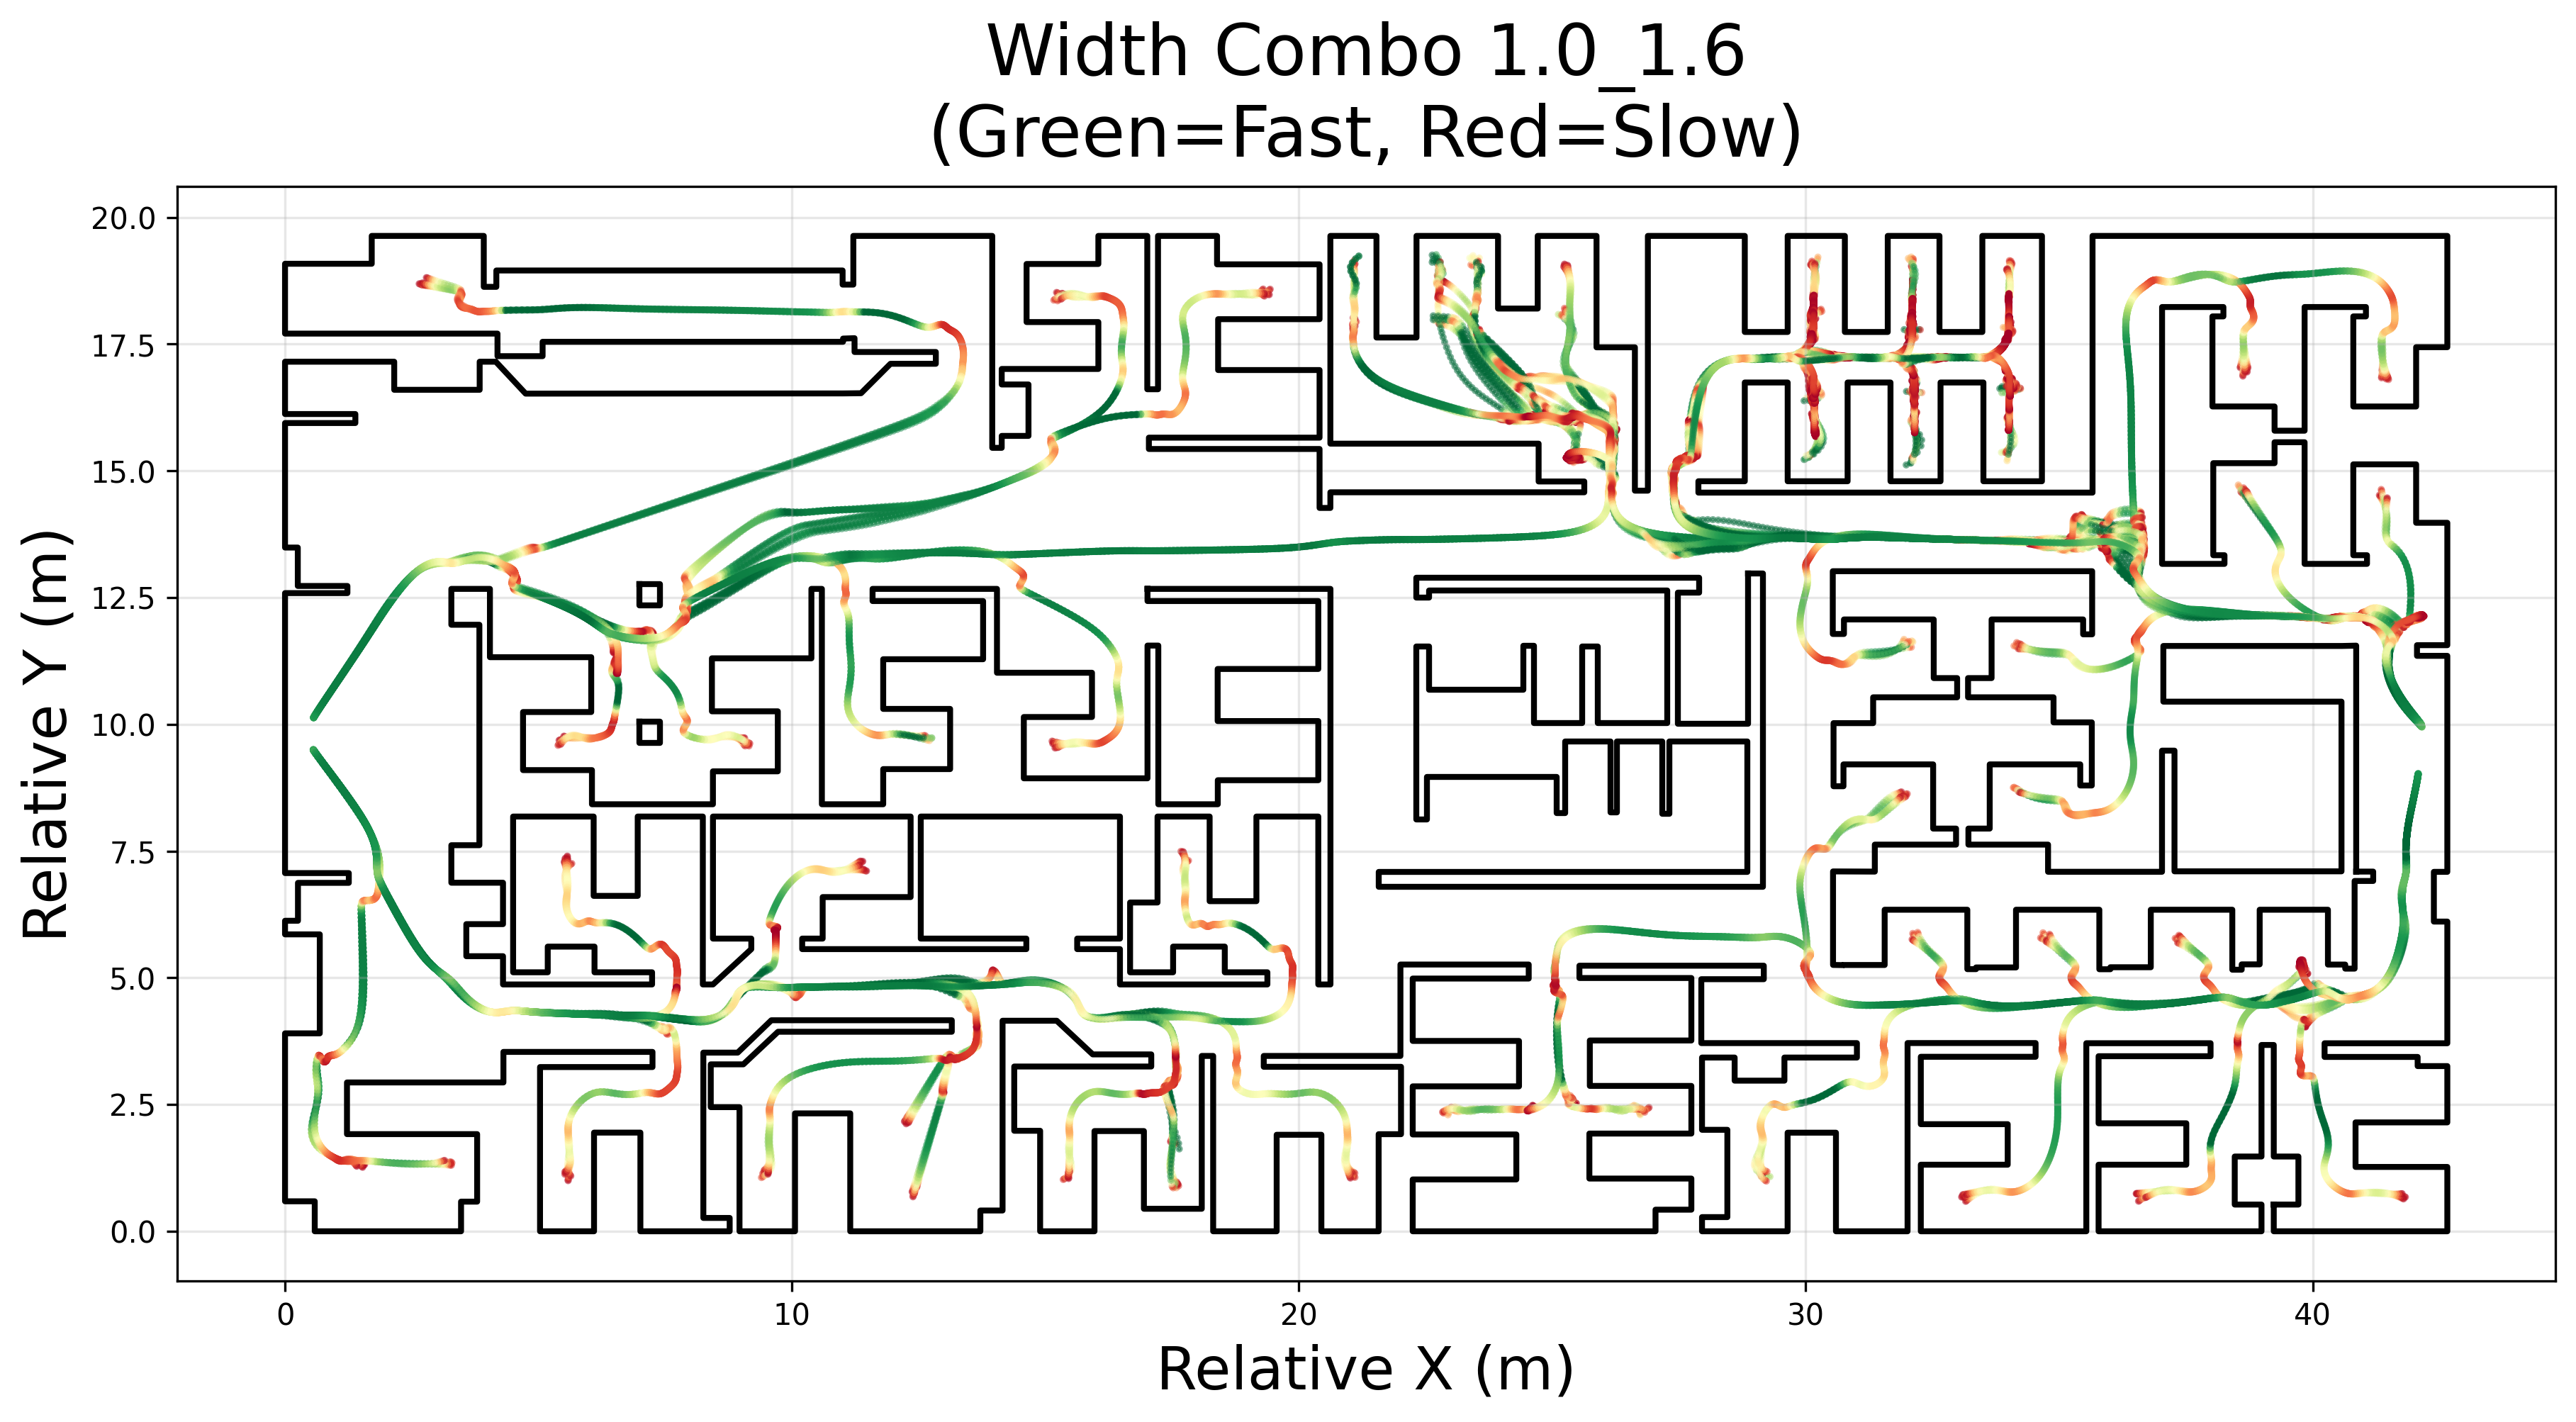
\includegraphics[width=\linewidth]{
            speed_trajectory_MultiRoom_width_1.0_1.6.png}
        \caption{Width Combo 1.0m and 1.6m}
        \label{fig:width_combo_1.0_1.6m}
    \end{subfigure}

    \caption{Speed and Trajectories for Room Door Width 1.0m}
    \label{fig:width_combo_1.0_x}
\end{figure}

\begin{figure}[h]
    \centering
    \begin{subfigure}[b]{.45\linewidth}
        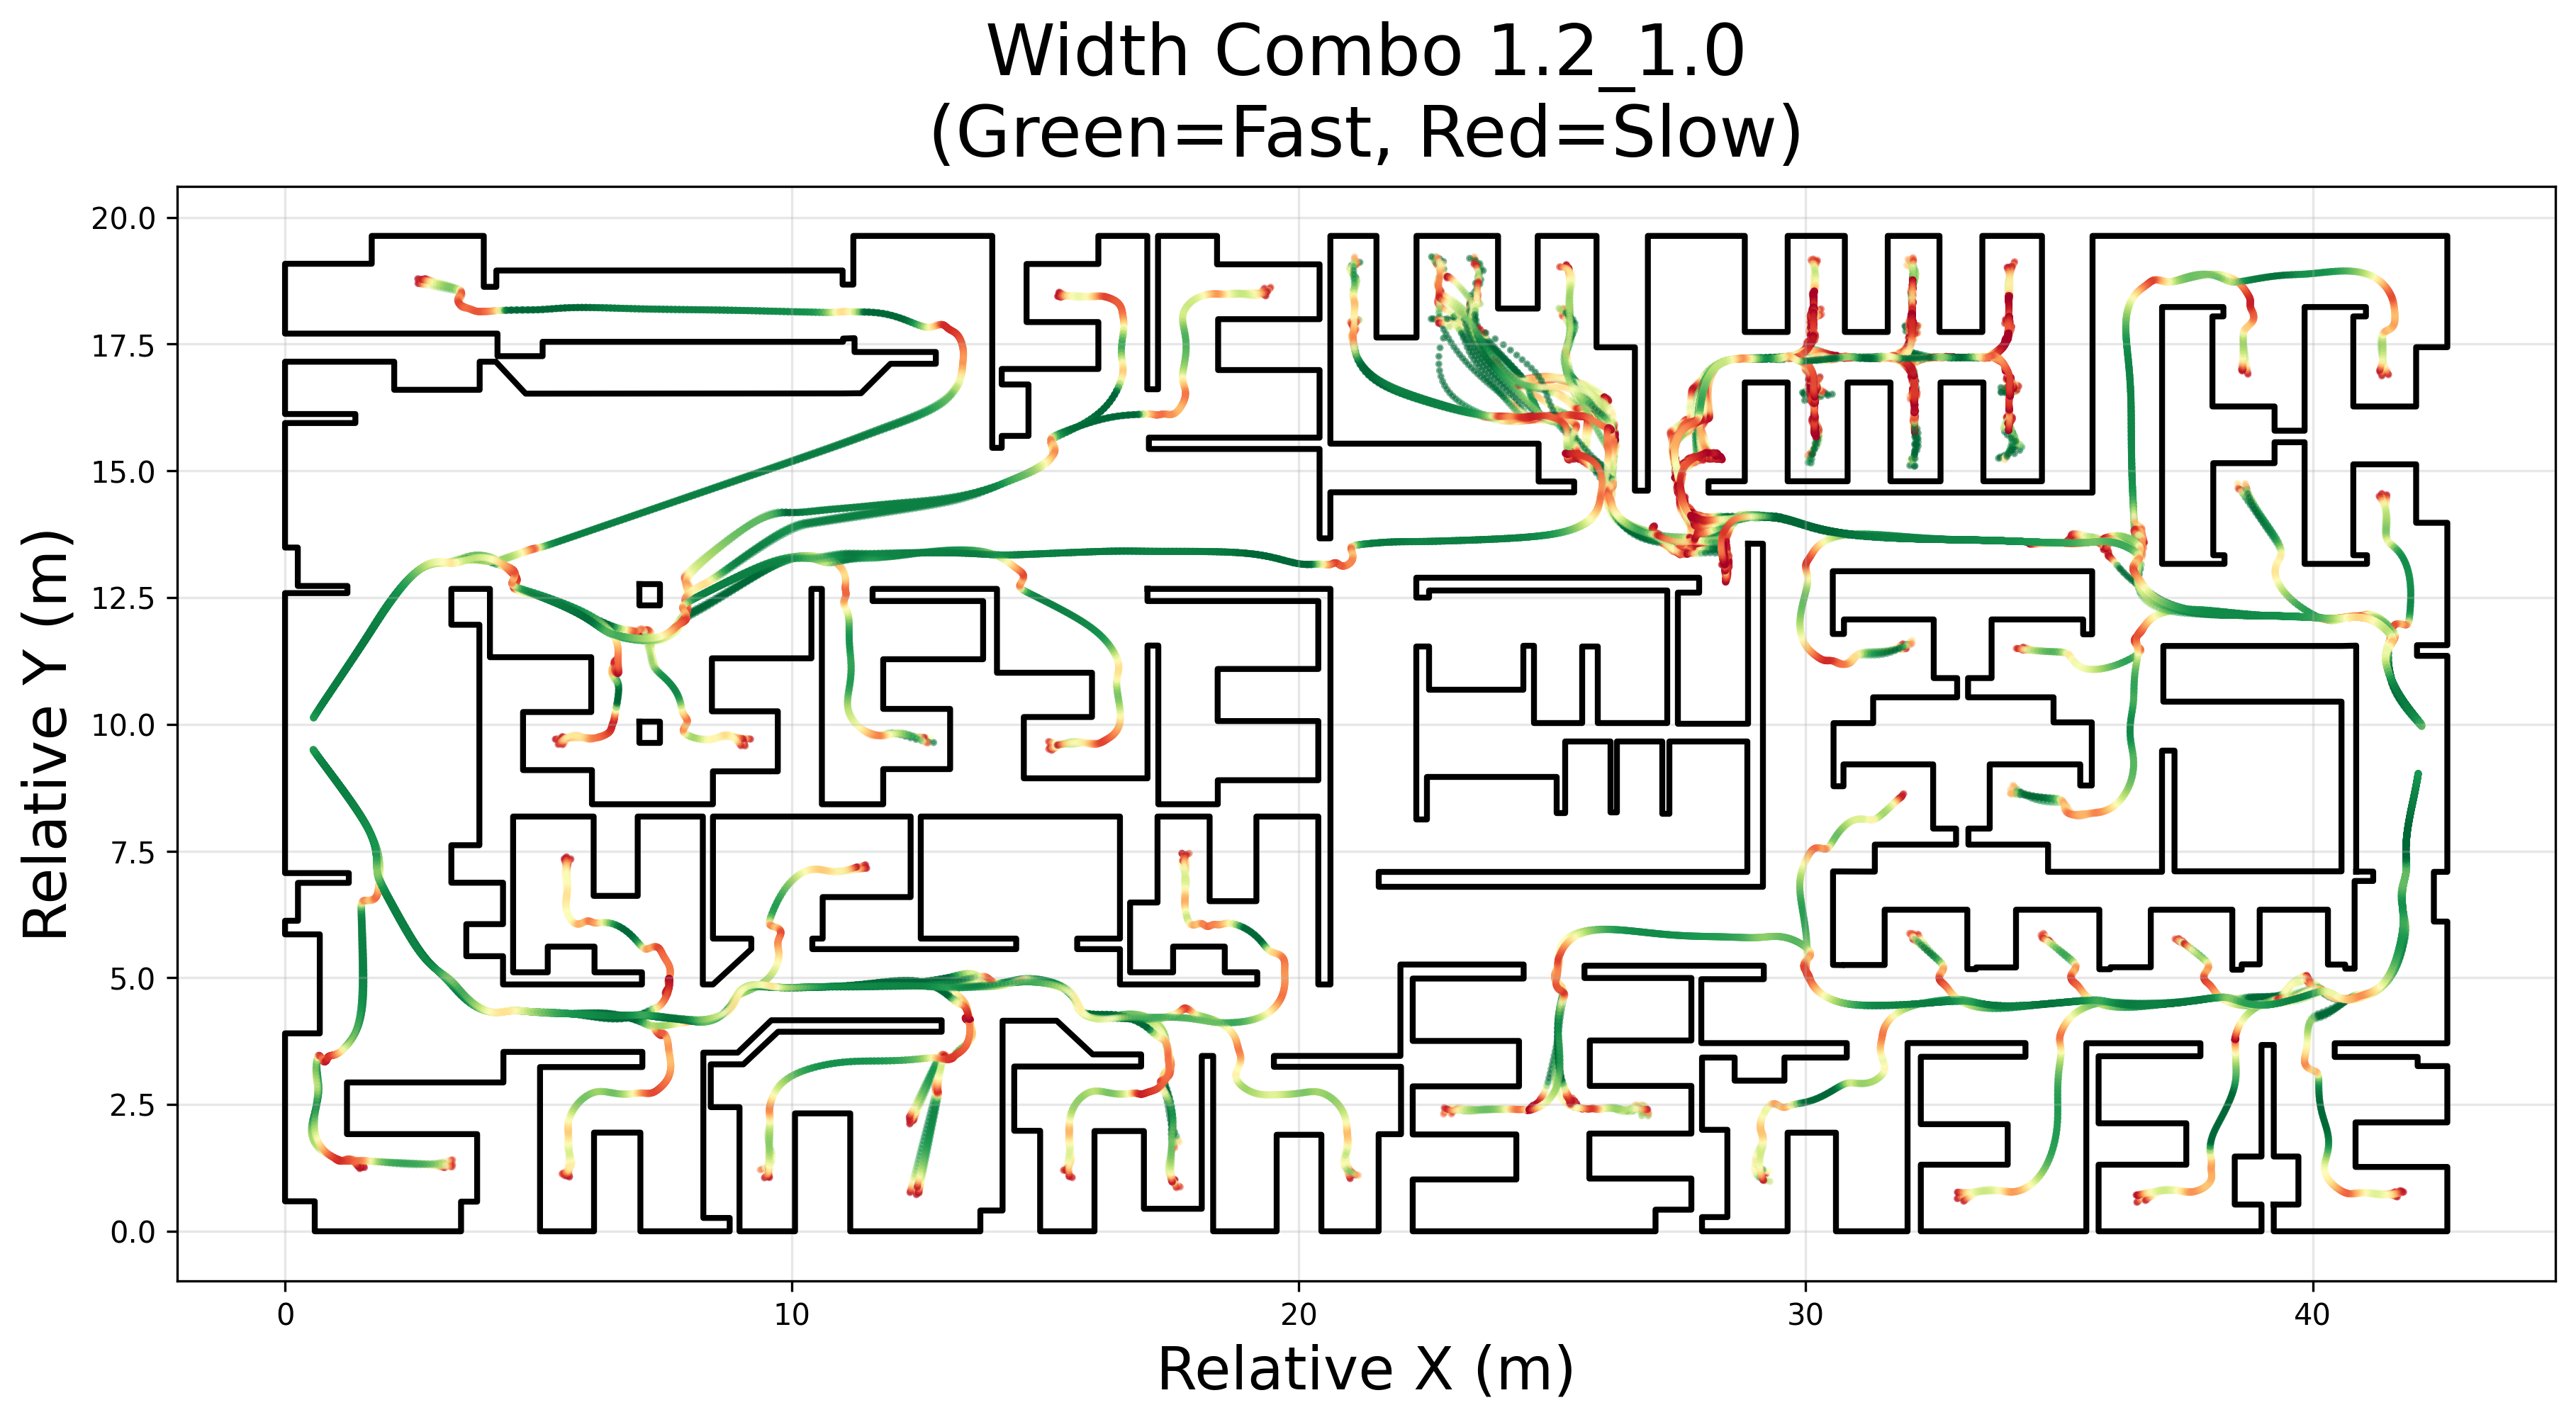
\includegraphics[width=\linewidth]{
            speed_trajectory_MultiRoom_width_1.2_1.0.png}
        \caption{Width Combo 1.2m and 1.0m}
        \label{fig:width_combo_1.2_1.0m}
    \end{subfigure}
    \begin{subfigure}[b]{.45\linewidth}
        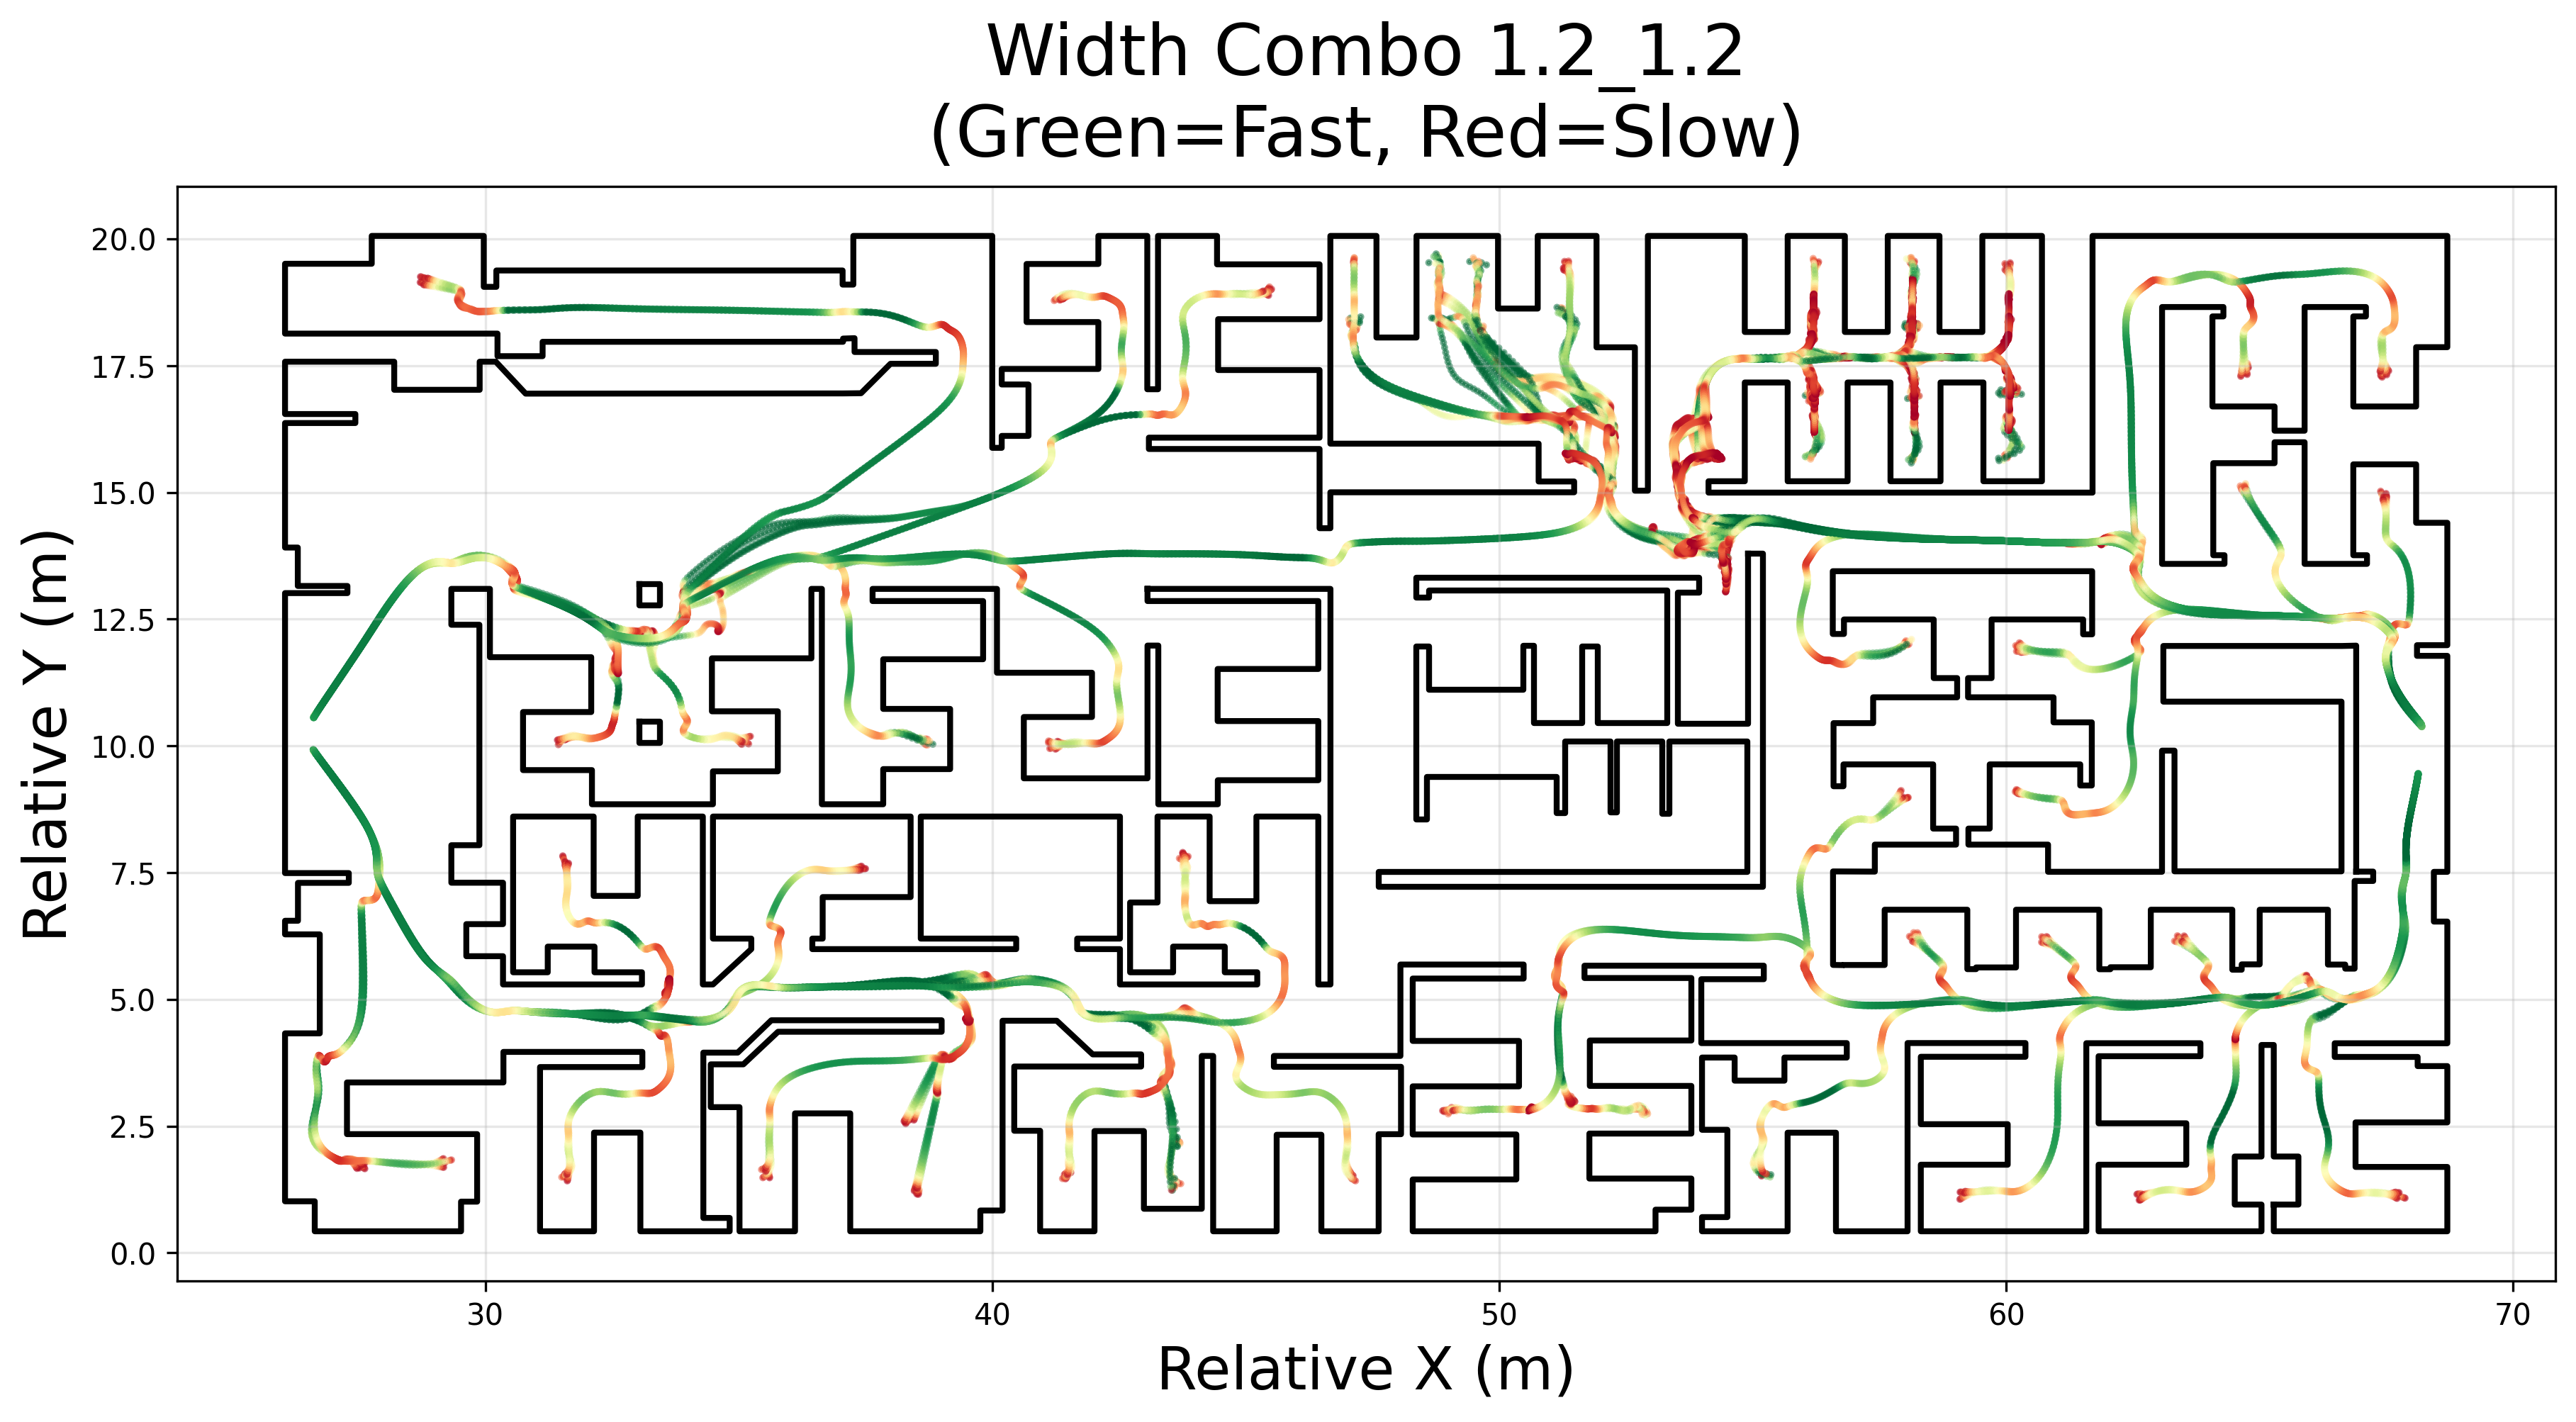
\includegraphics[width=\linewidth]{
            speed_trajectory_MultiRoom_width_1.2_1.2.png}
        \caption{Width Combo 1.2m and 1.2m}
        \label{fig:width_combo_1.2_1.2m}
    \end{subfigure}

    \begin{subfigure}[b]{.45\linewidth}
        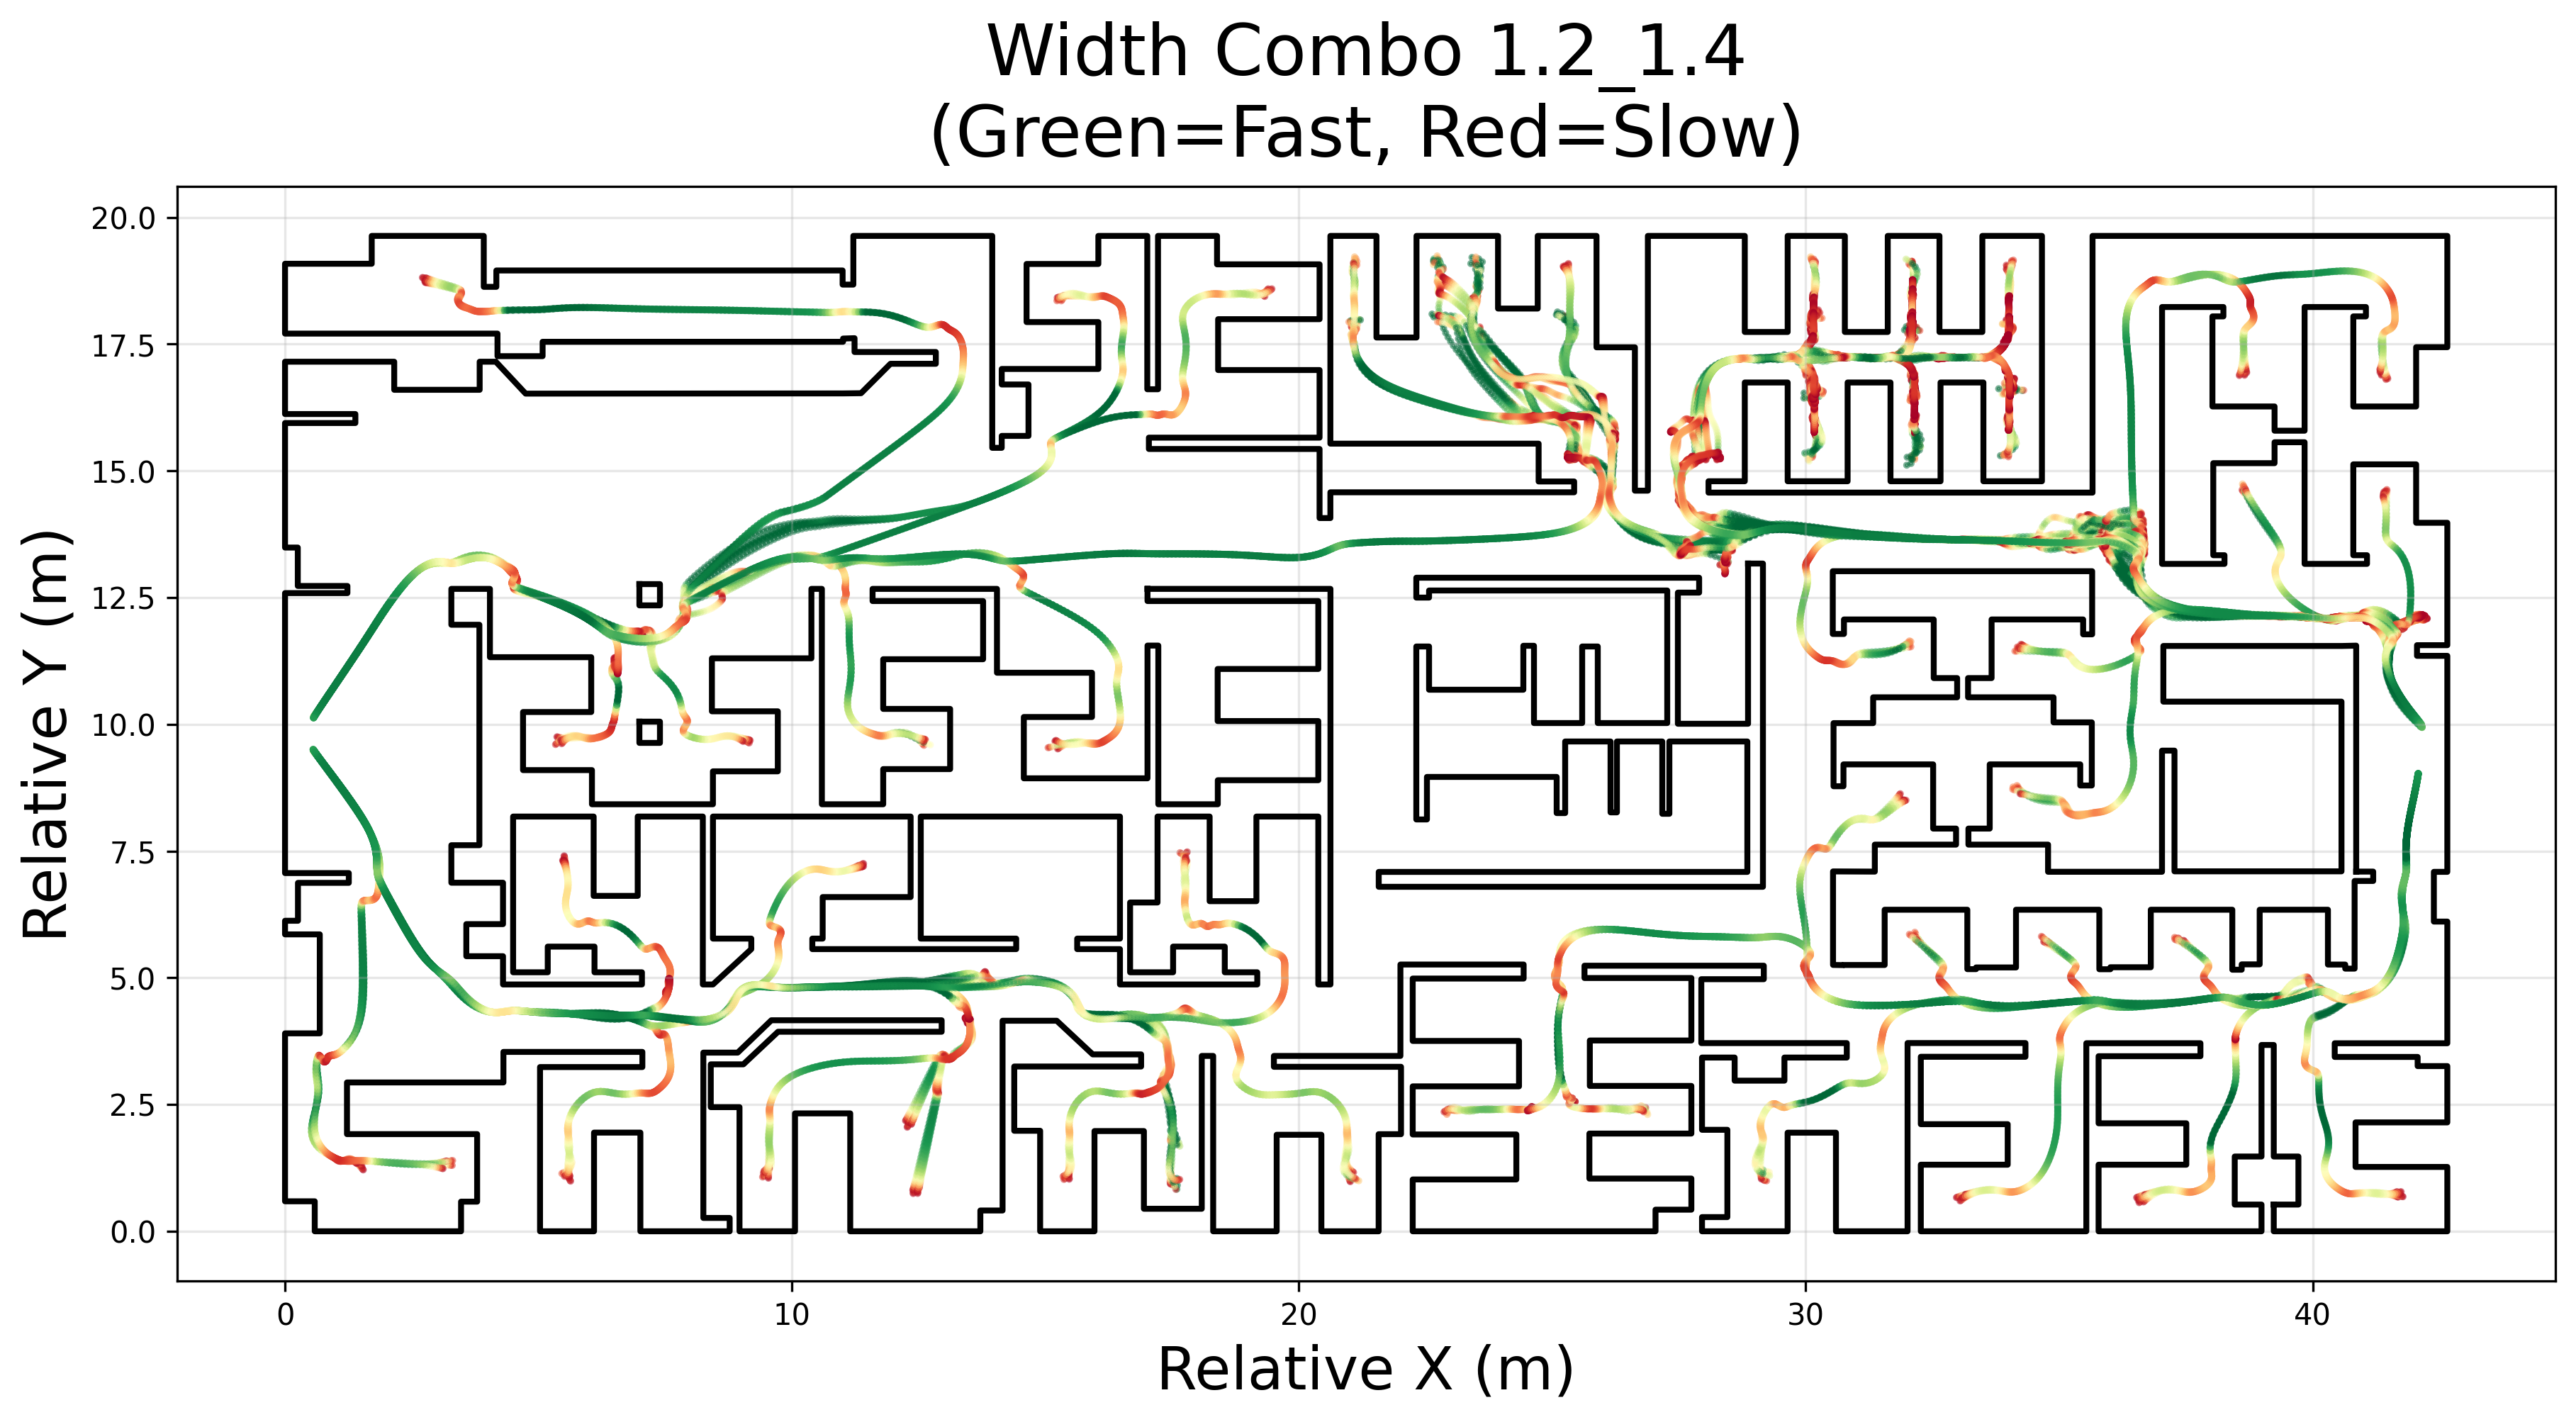
\includegraphics[width=\linewidth]{
            speed_trajectory_MultiRoom_width_1.2_1.4.png}
        \caption{Width Combo 1.2m and 1.4m}
        \label{fig:width_combo_1.2_1.4m}
    \end{subfigure}
    \begin{subfigure}[b]{.45\linewidth}
        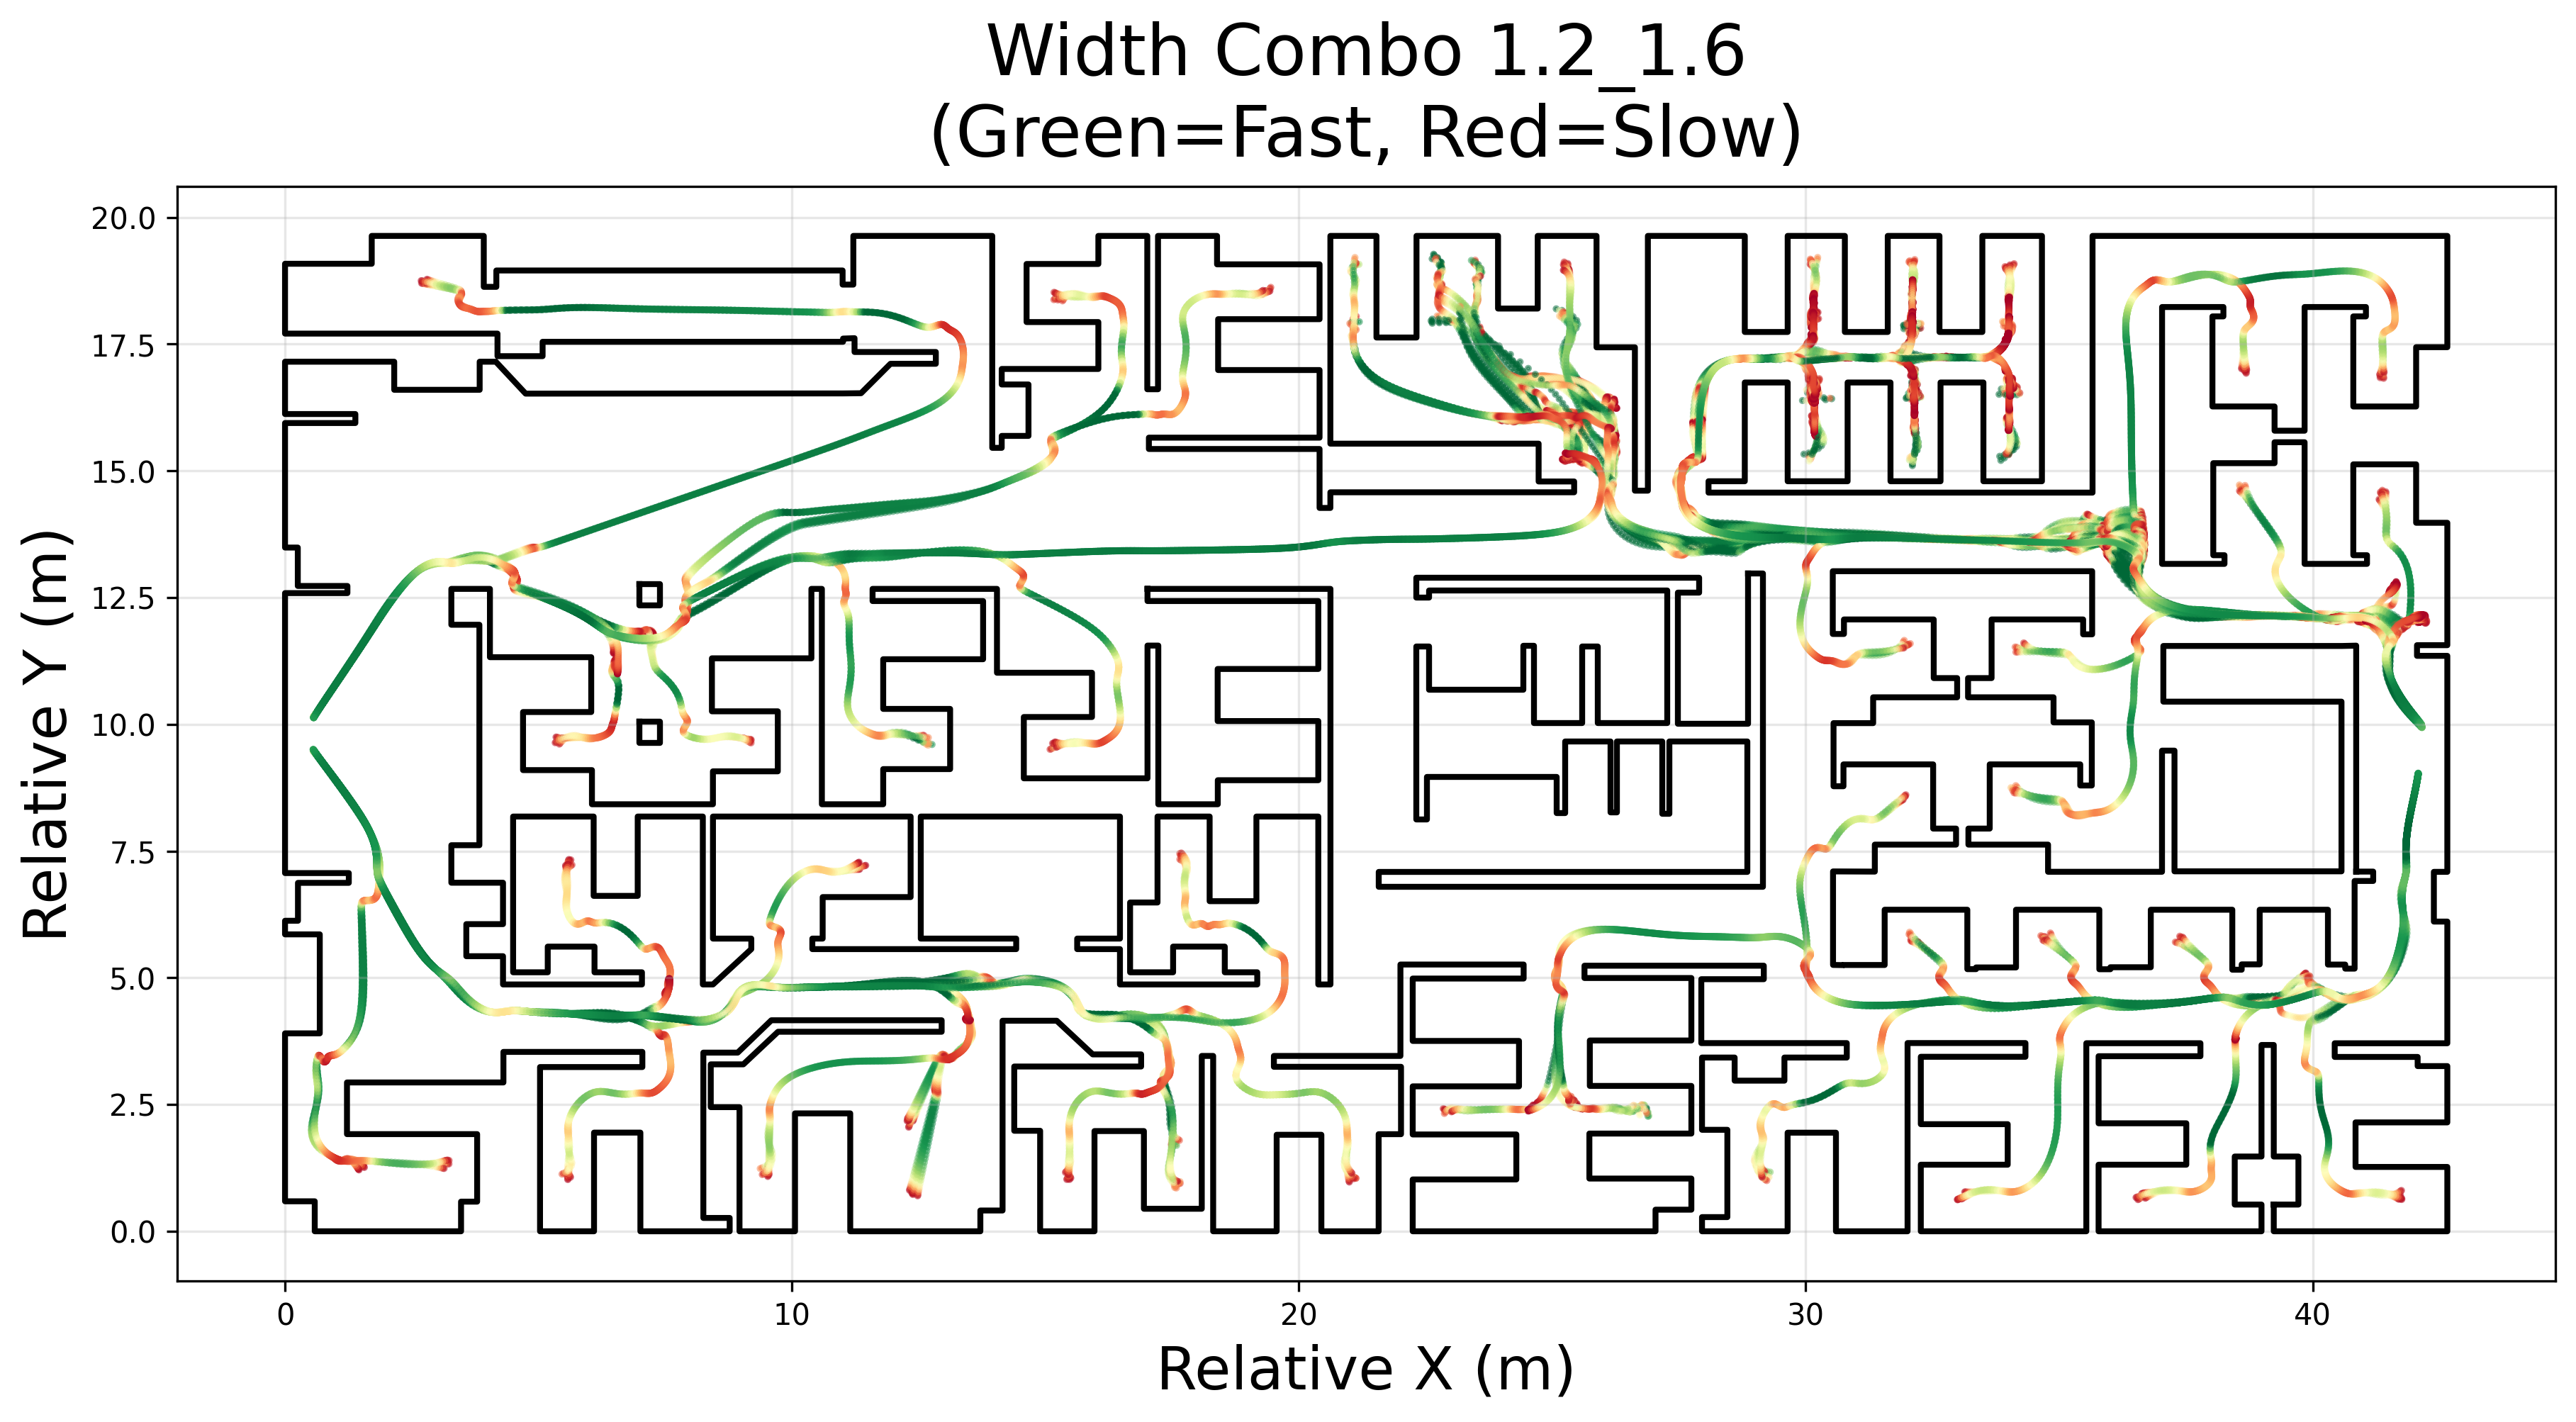
\includegraphics[width=\linewidth]{
            speed_trajectory_MultiRoom_width_1.2_1.6.png}
        \caption{Width Combo 1.2m and 1.6m}
        \label{fig:width_combo_1.2_1.6m}
    \end{subfigure}

    \caption{Speed and Trajectories for Room Door Width 1.2m}
    \label{fig:width_combo_1.2_x}
\end{figure}

\begin{figure}[h]
    \centering
        \begin{subfigure}[b]{.45\linewidth}
        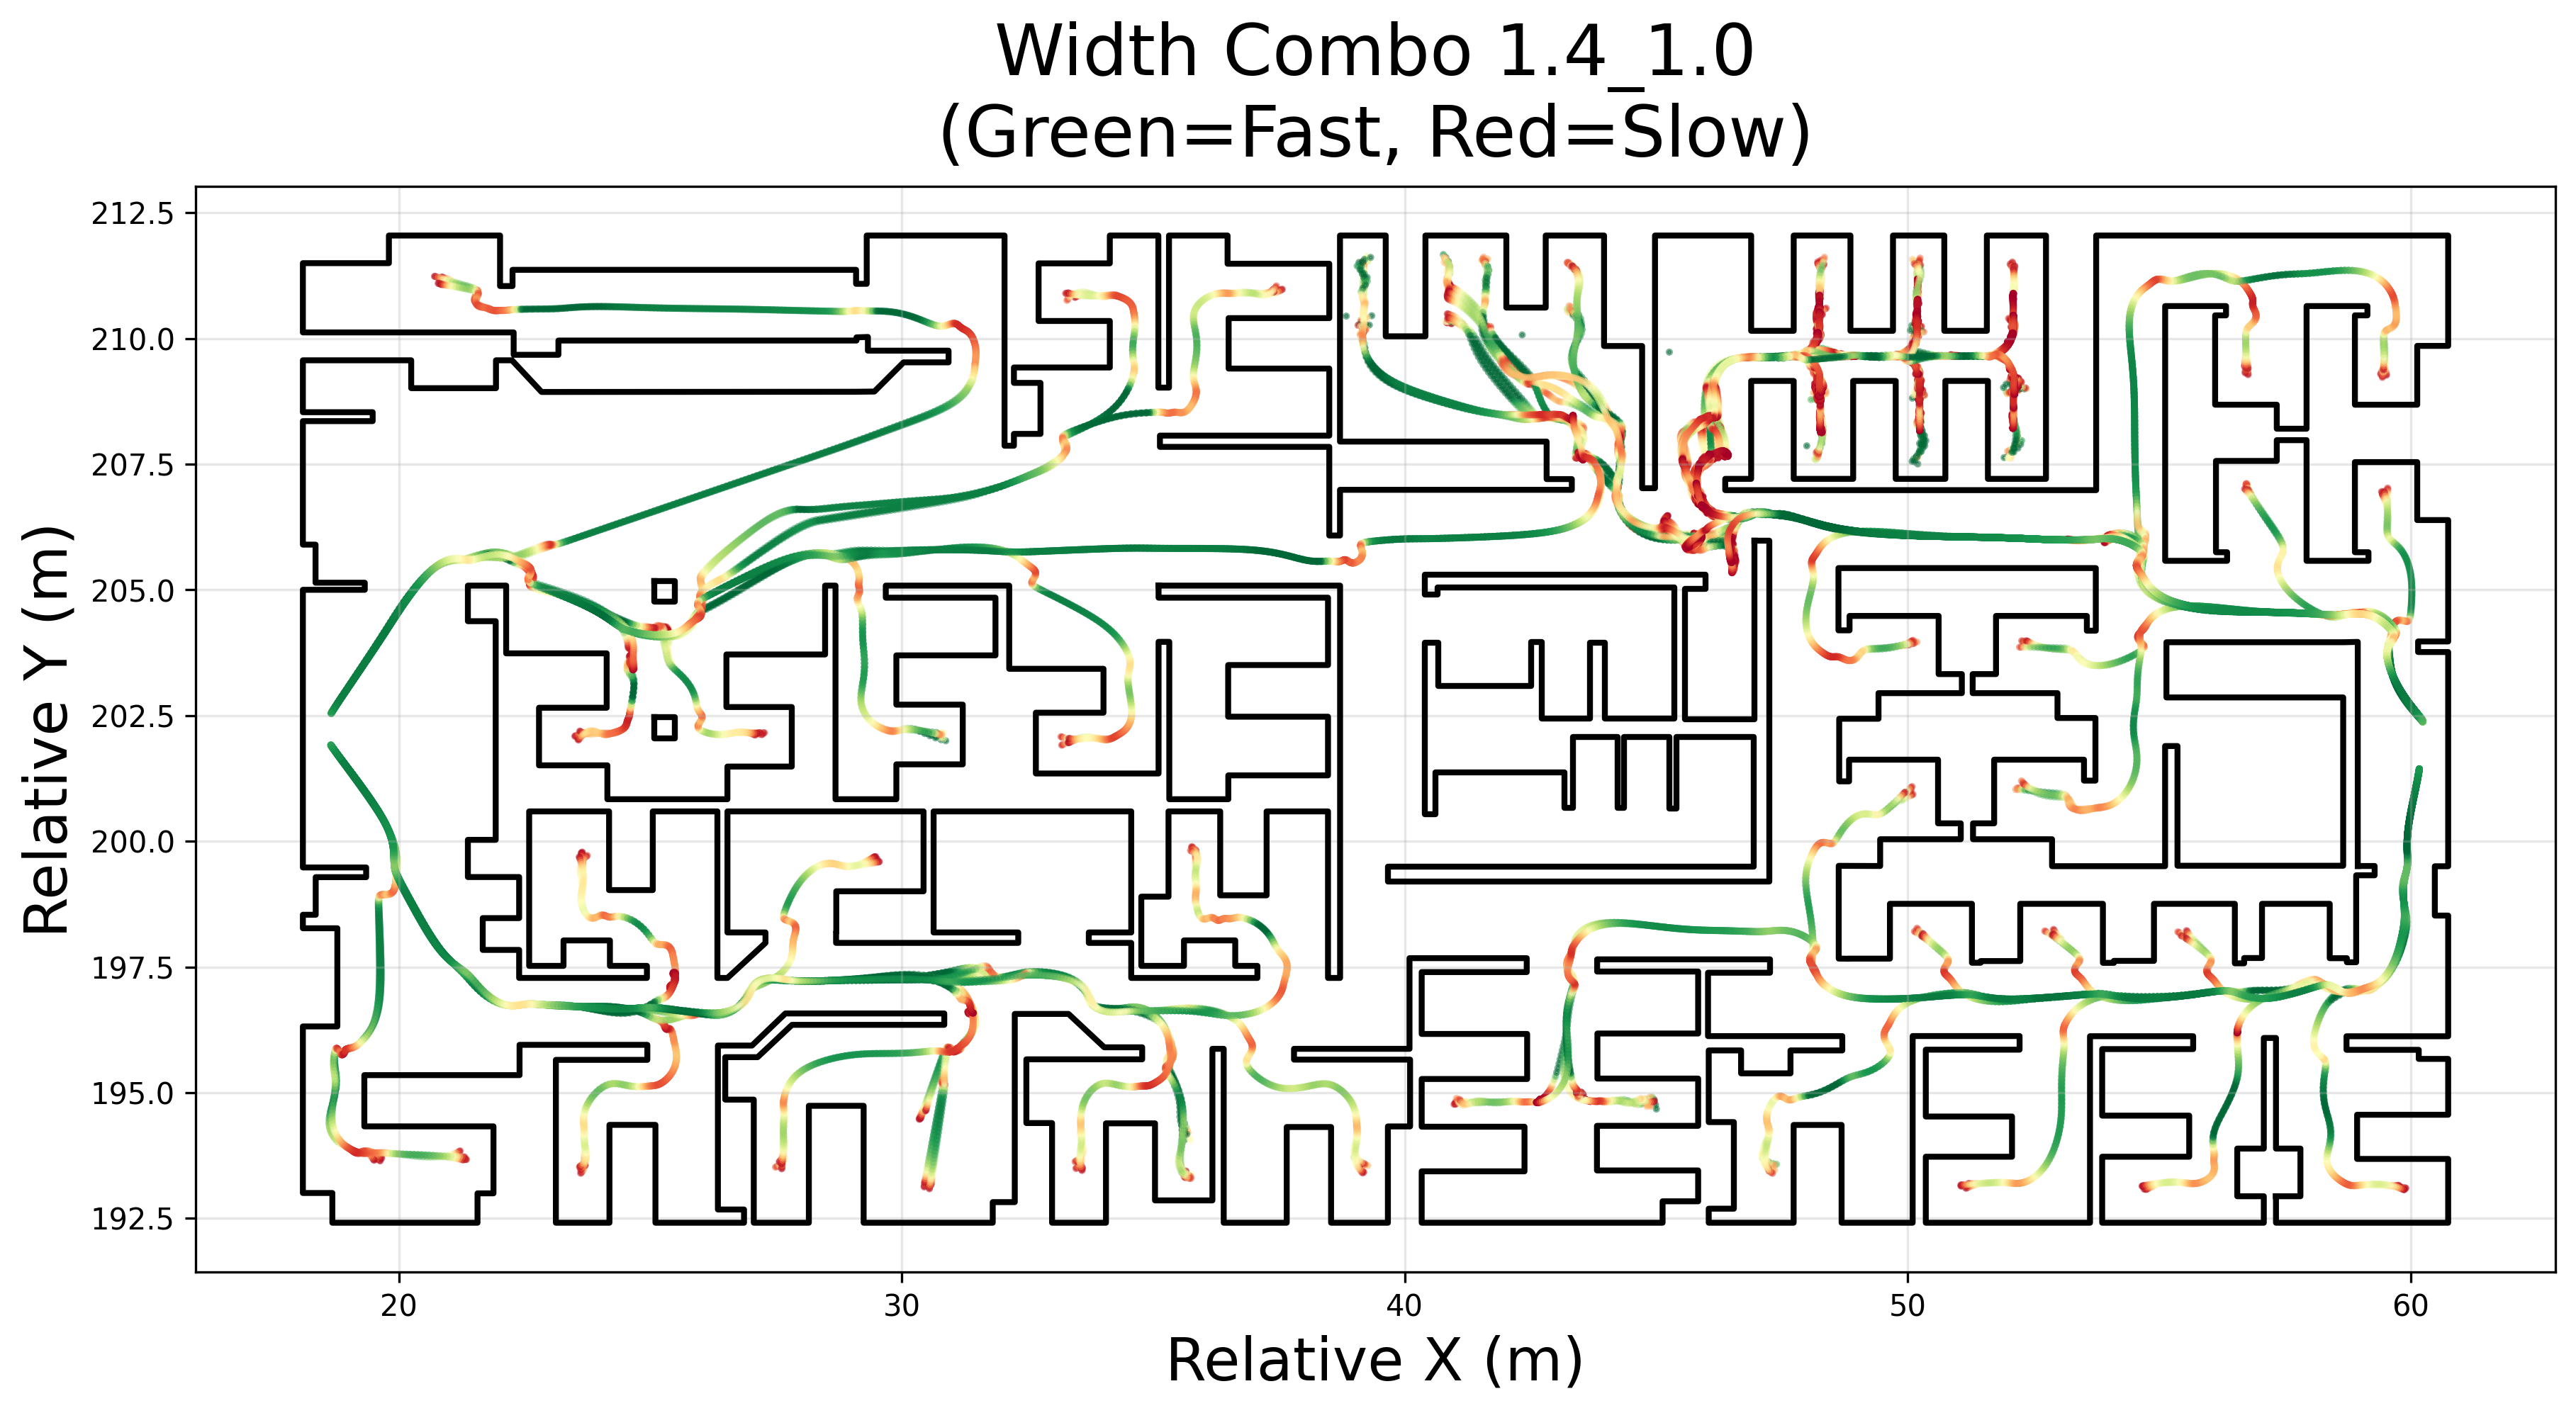
\includegraphics[width=\linewidth]{
            speed_trajectory_MultiRoom_width_1.4_1.0.png}
        \caption{Width Combo 1.4m and 1.0m}
        \label{fig:width_combo_1.4_1.0m}
    \end{subfigure}
    \begin{subfigure}[b]{.45\linewidth}
        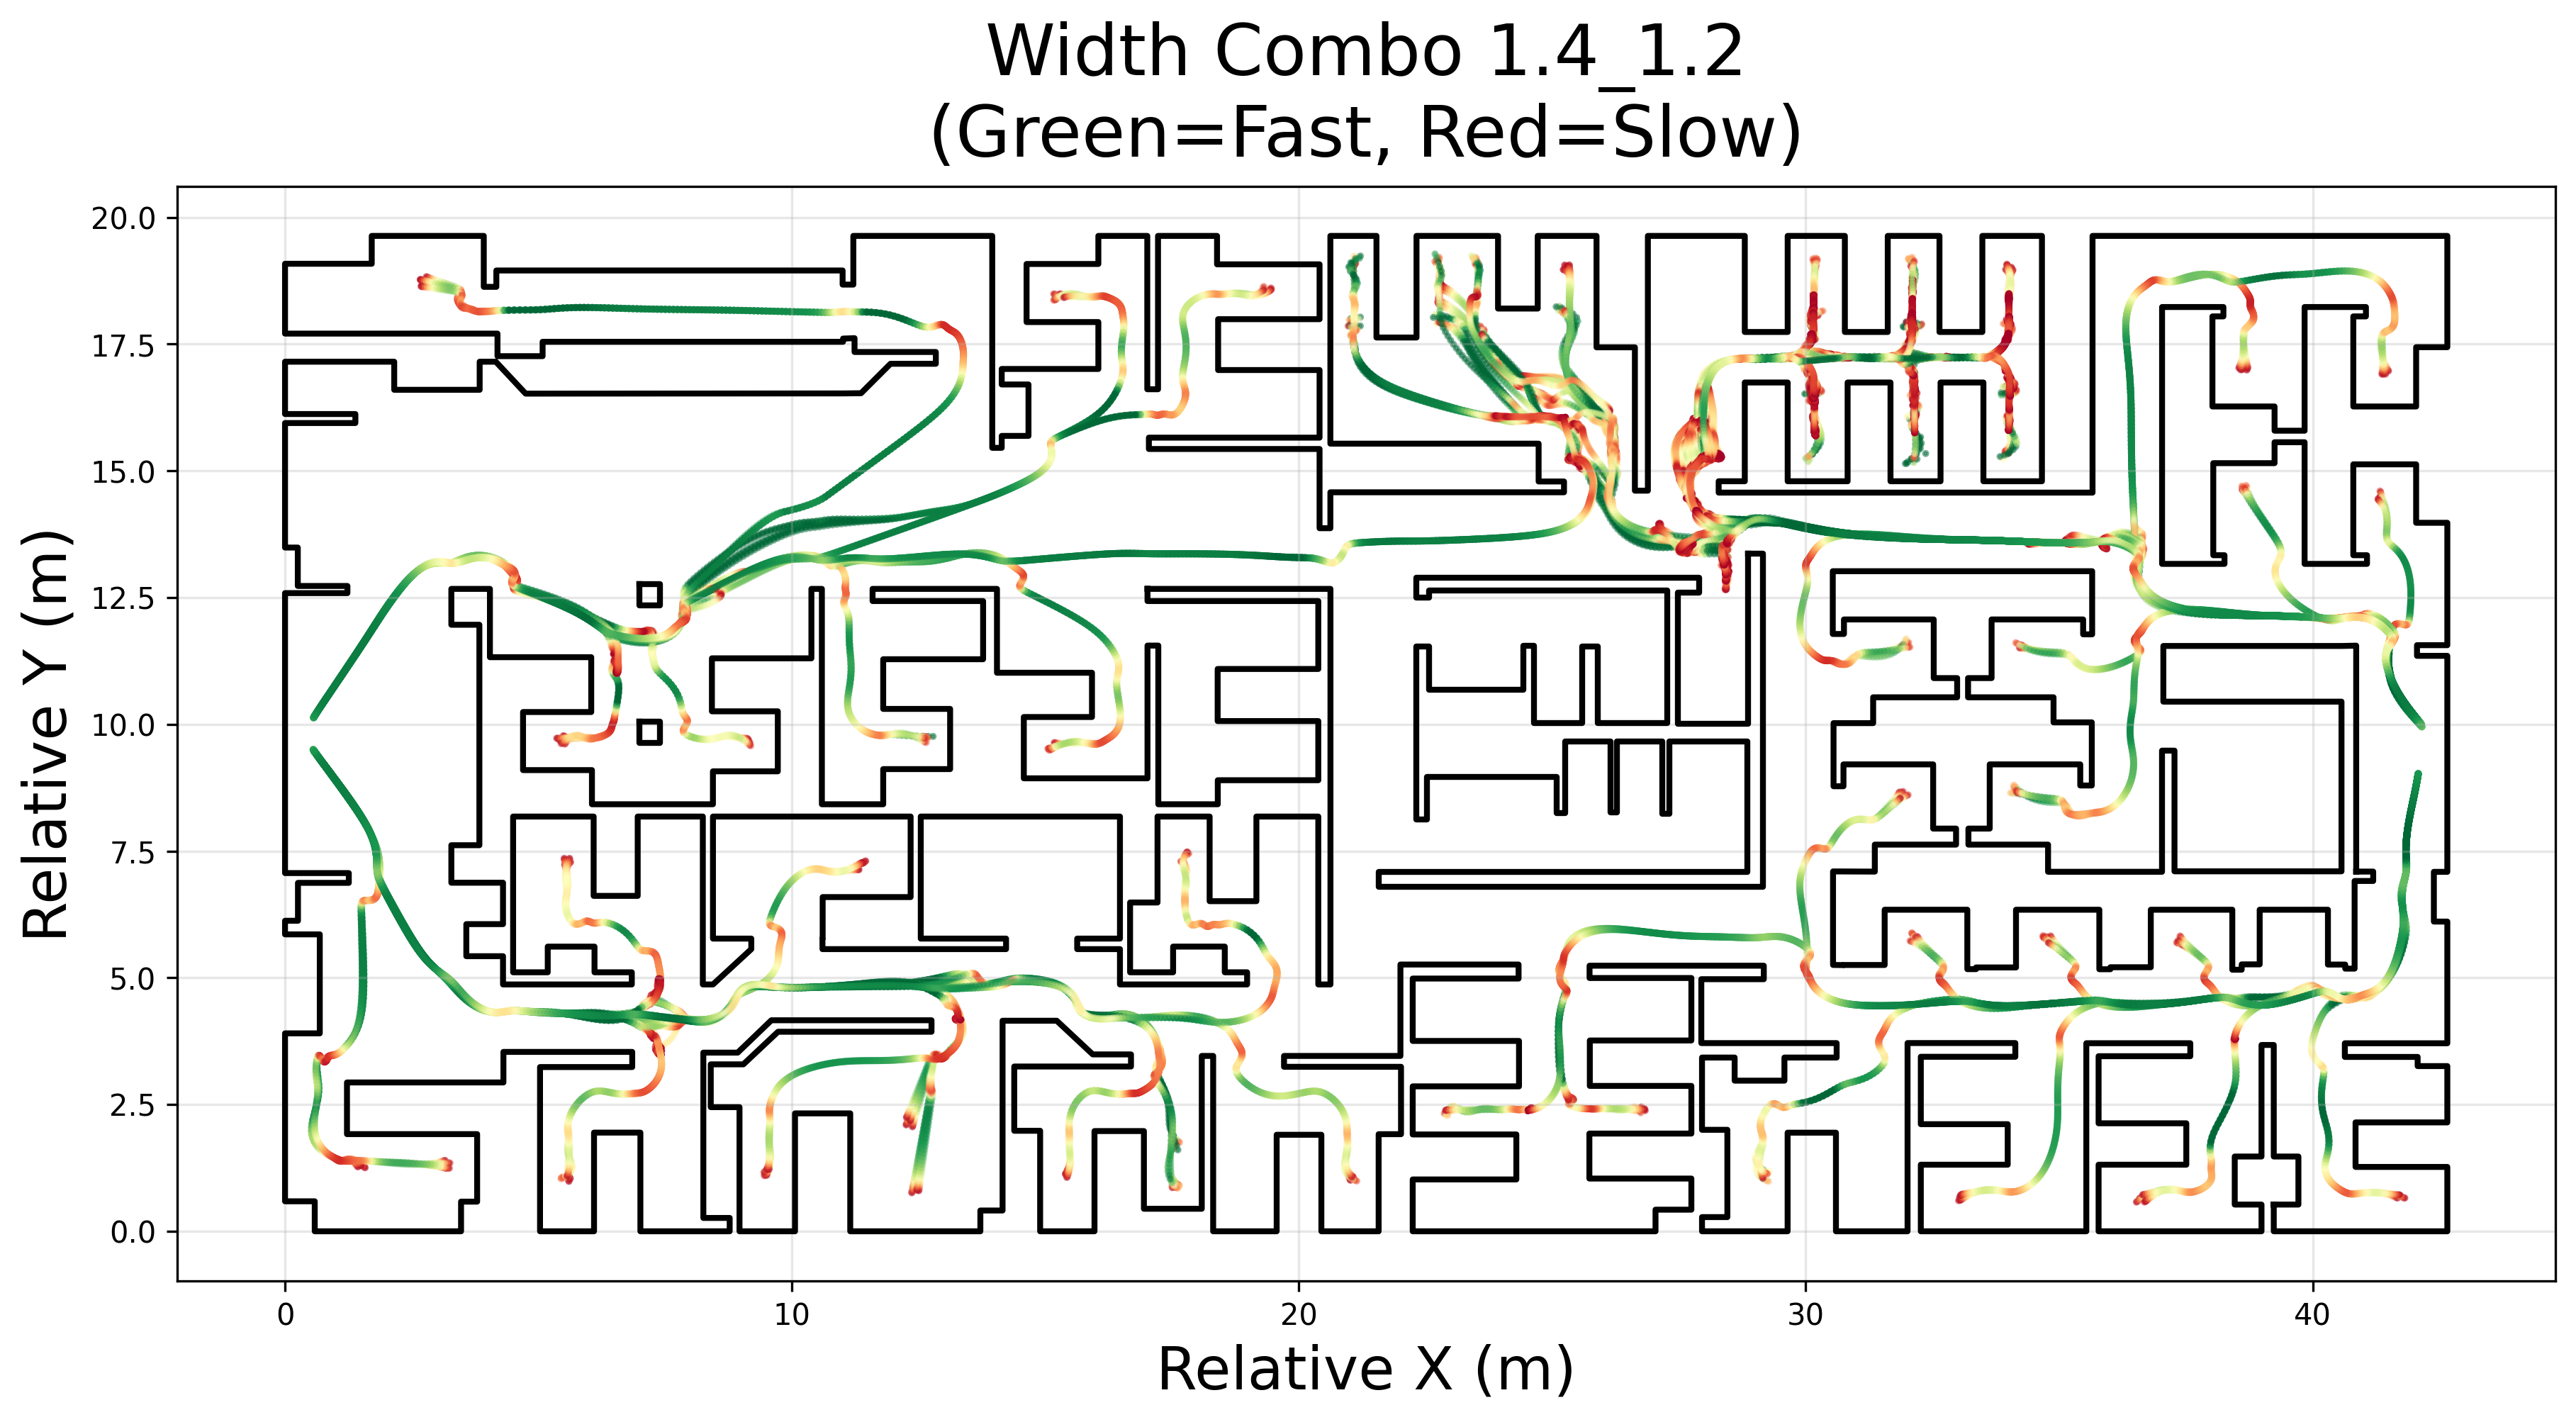
\includegraphics[width=\linewidth]{
            speed_trajectory_MultiRoom_width_1.4_1.2.png}
        \caption{Width Combo 1.4m and 1.2m}
        \label{fig:width_combo_1.4_1.2m}
    \end{subfigure}

    \begin{subfigure}[b]{.45\linewidth}
        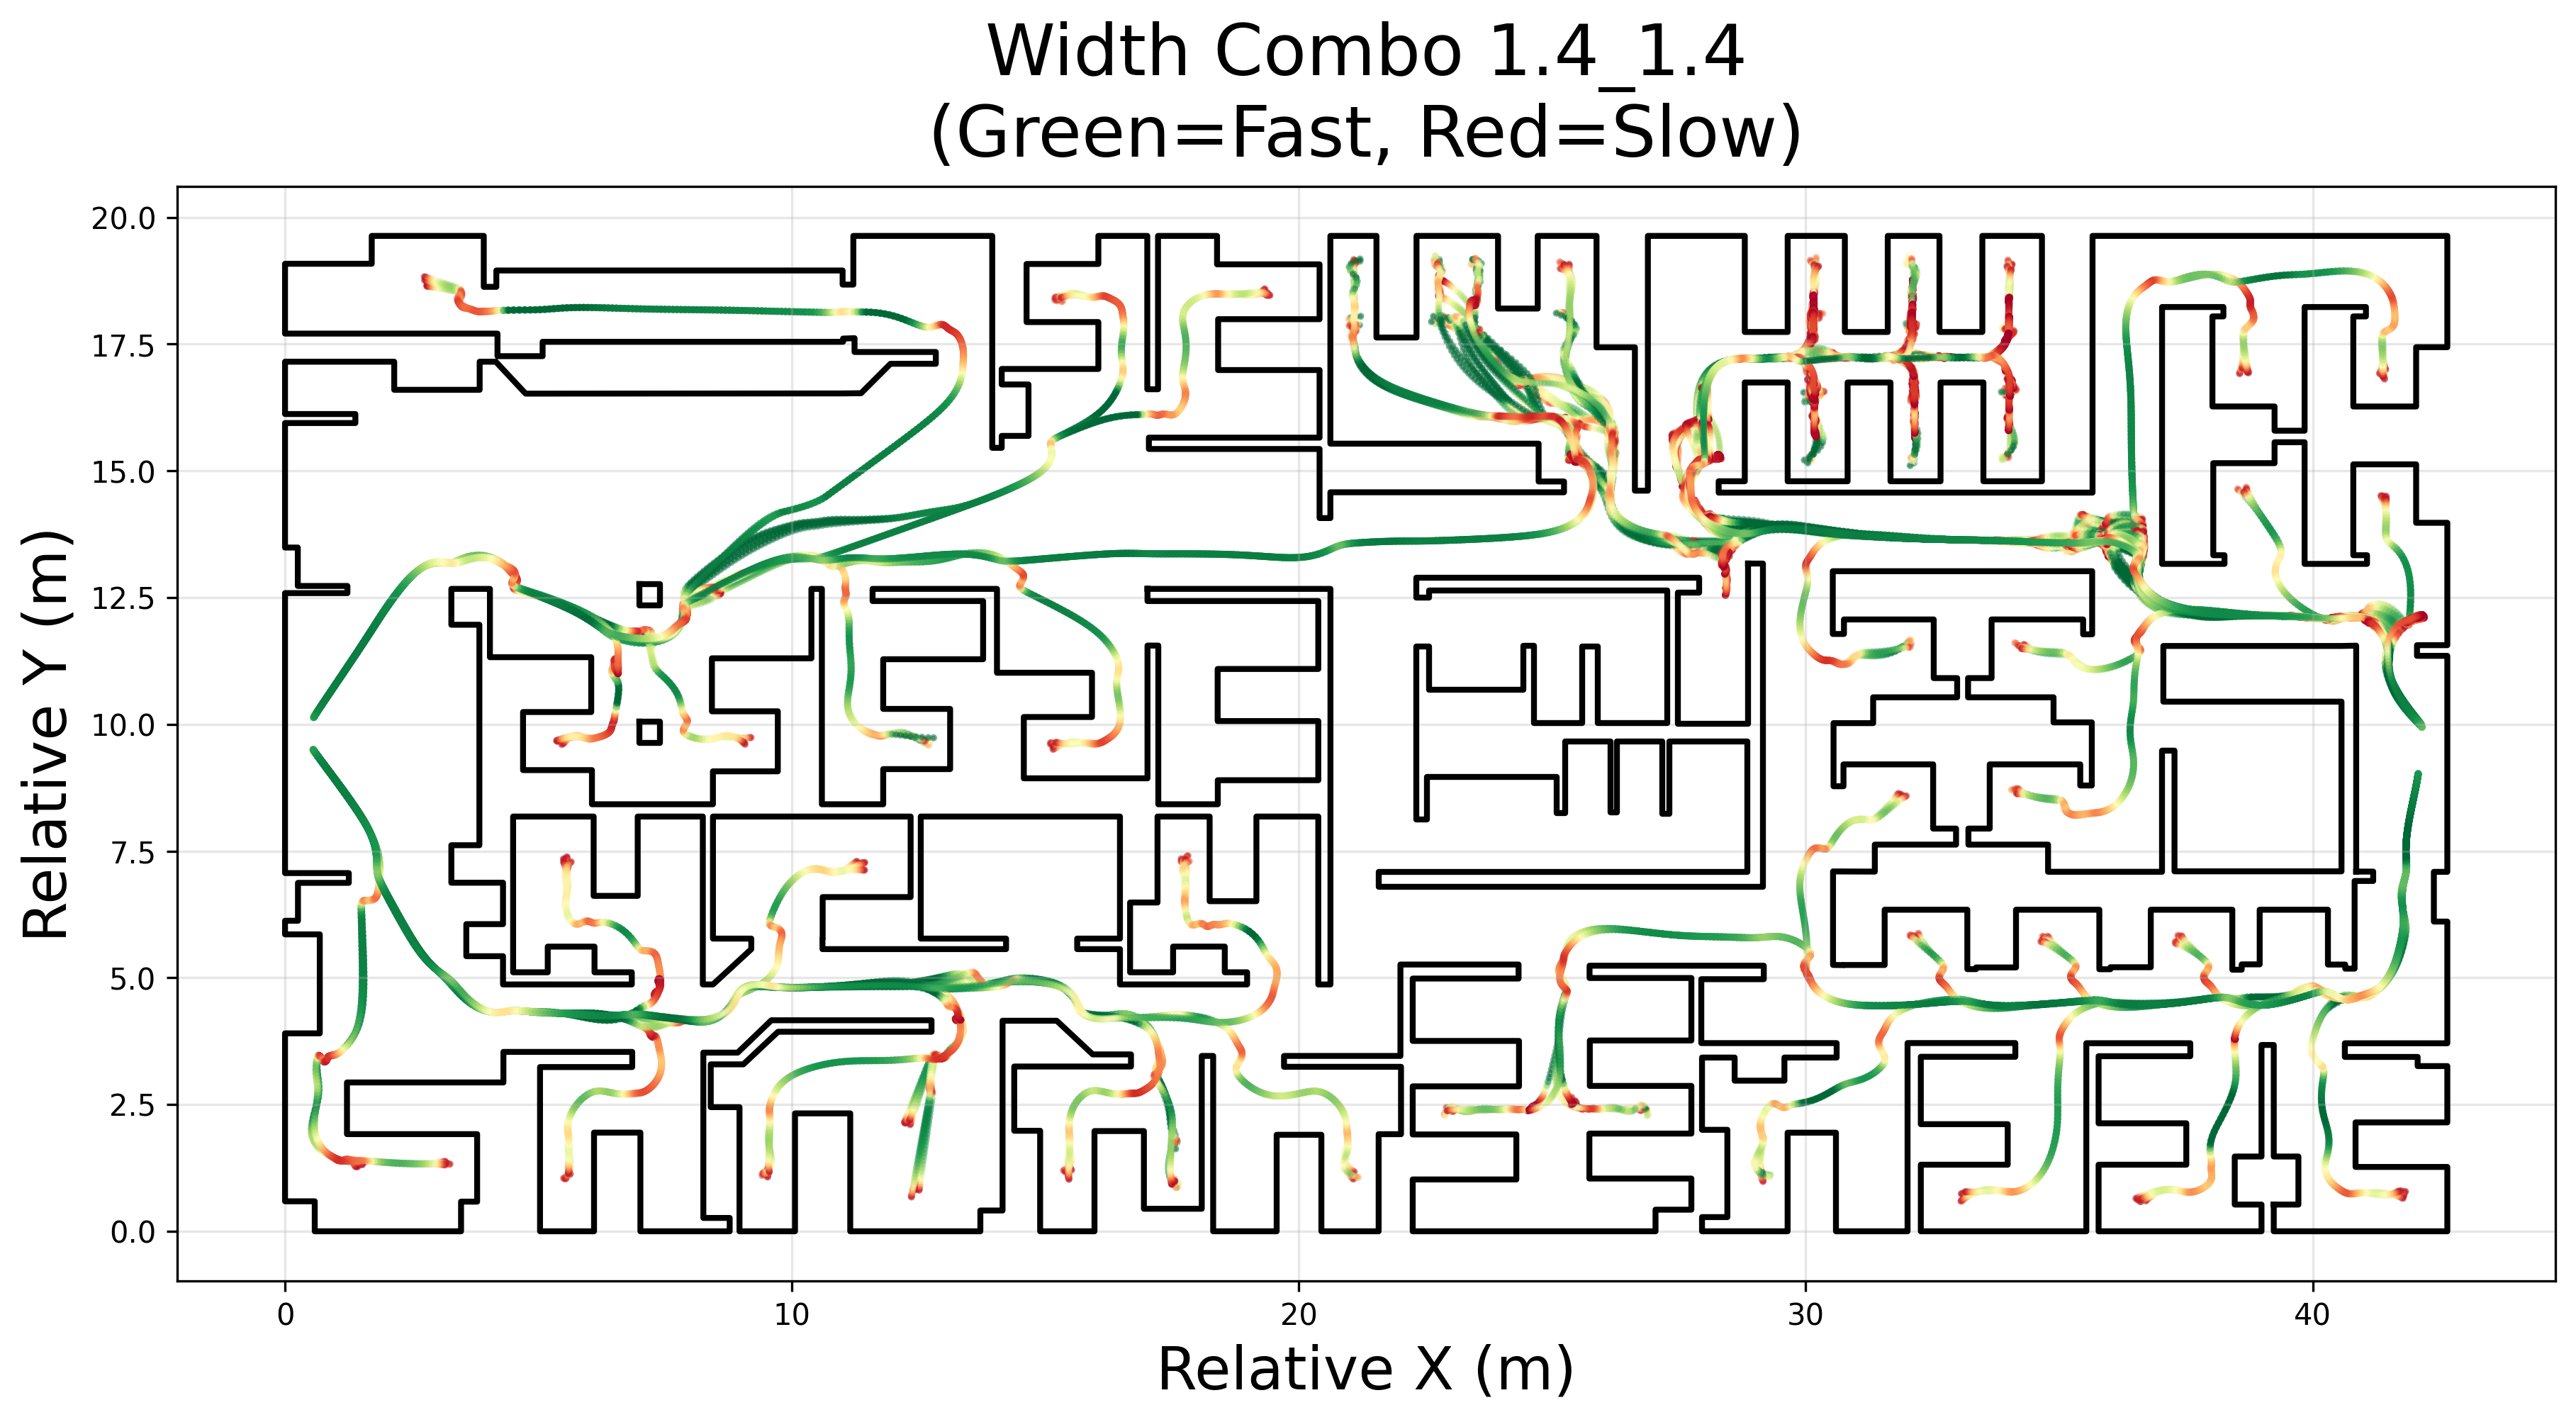
\includegraphics[width=\linewidth]{
            speed_trajectory_MultiRoom_width_1.4_1.4.png}
        \caption{Width Combo 1.4m and 1.4m}
        \label{fig:width_combo_1.4_1.4m}
    \end{subfigure}
    \begin{subfigure}[b]{.45\linewidth}
        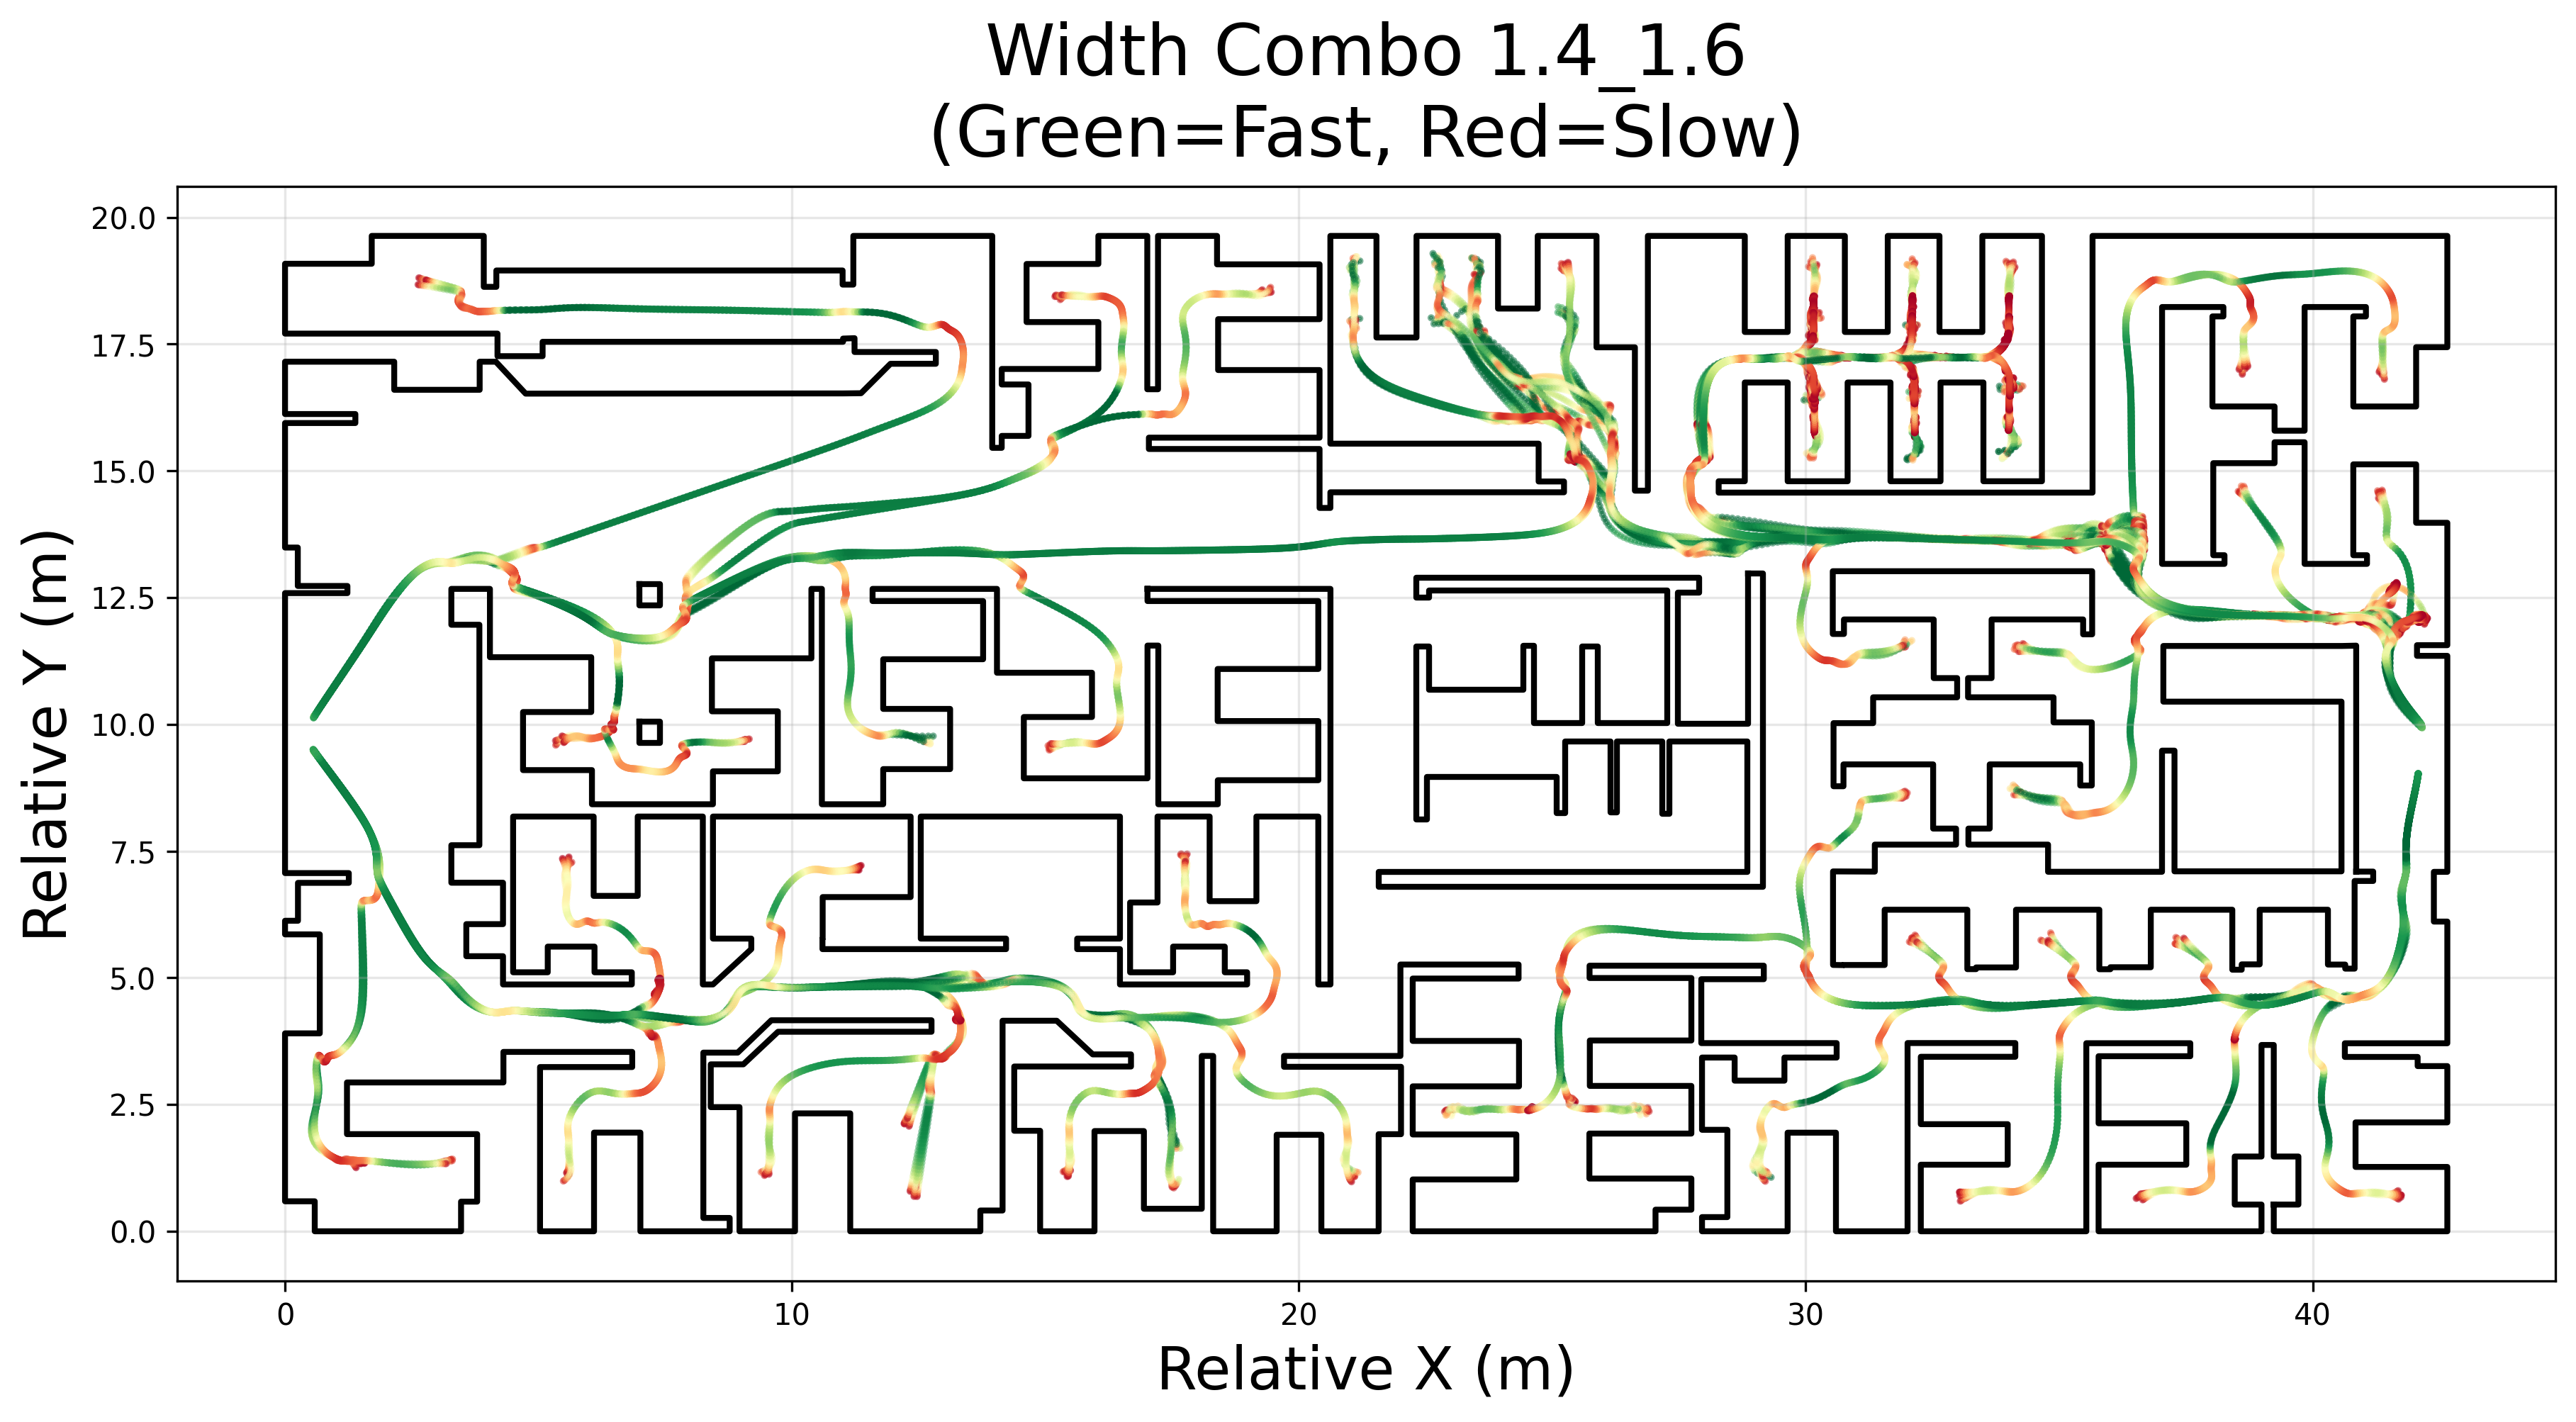
\includegraphics[width=\linewidth]{
            speed_trajectory_MultiRoom_width_1.4_1.6.png}
        \caption{Width Combo 1.4m and 1.6m}
        \label{fig:width_combo_1.4_1.6m}
    \end{subfigure}
    
    \caption{Speed and Trajectories for Room Door Width 1.4m}
    \label{fig:width_combo_1.4_x}
\end{figure}

\begin{figure}[h]
    \centering
        \begin{subfigure}[b]{.45\linewidth}
        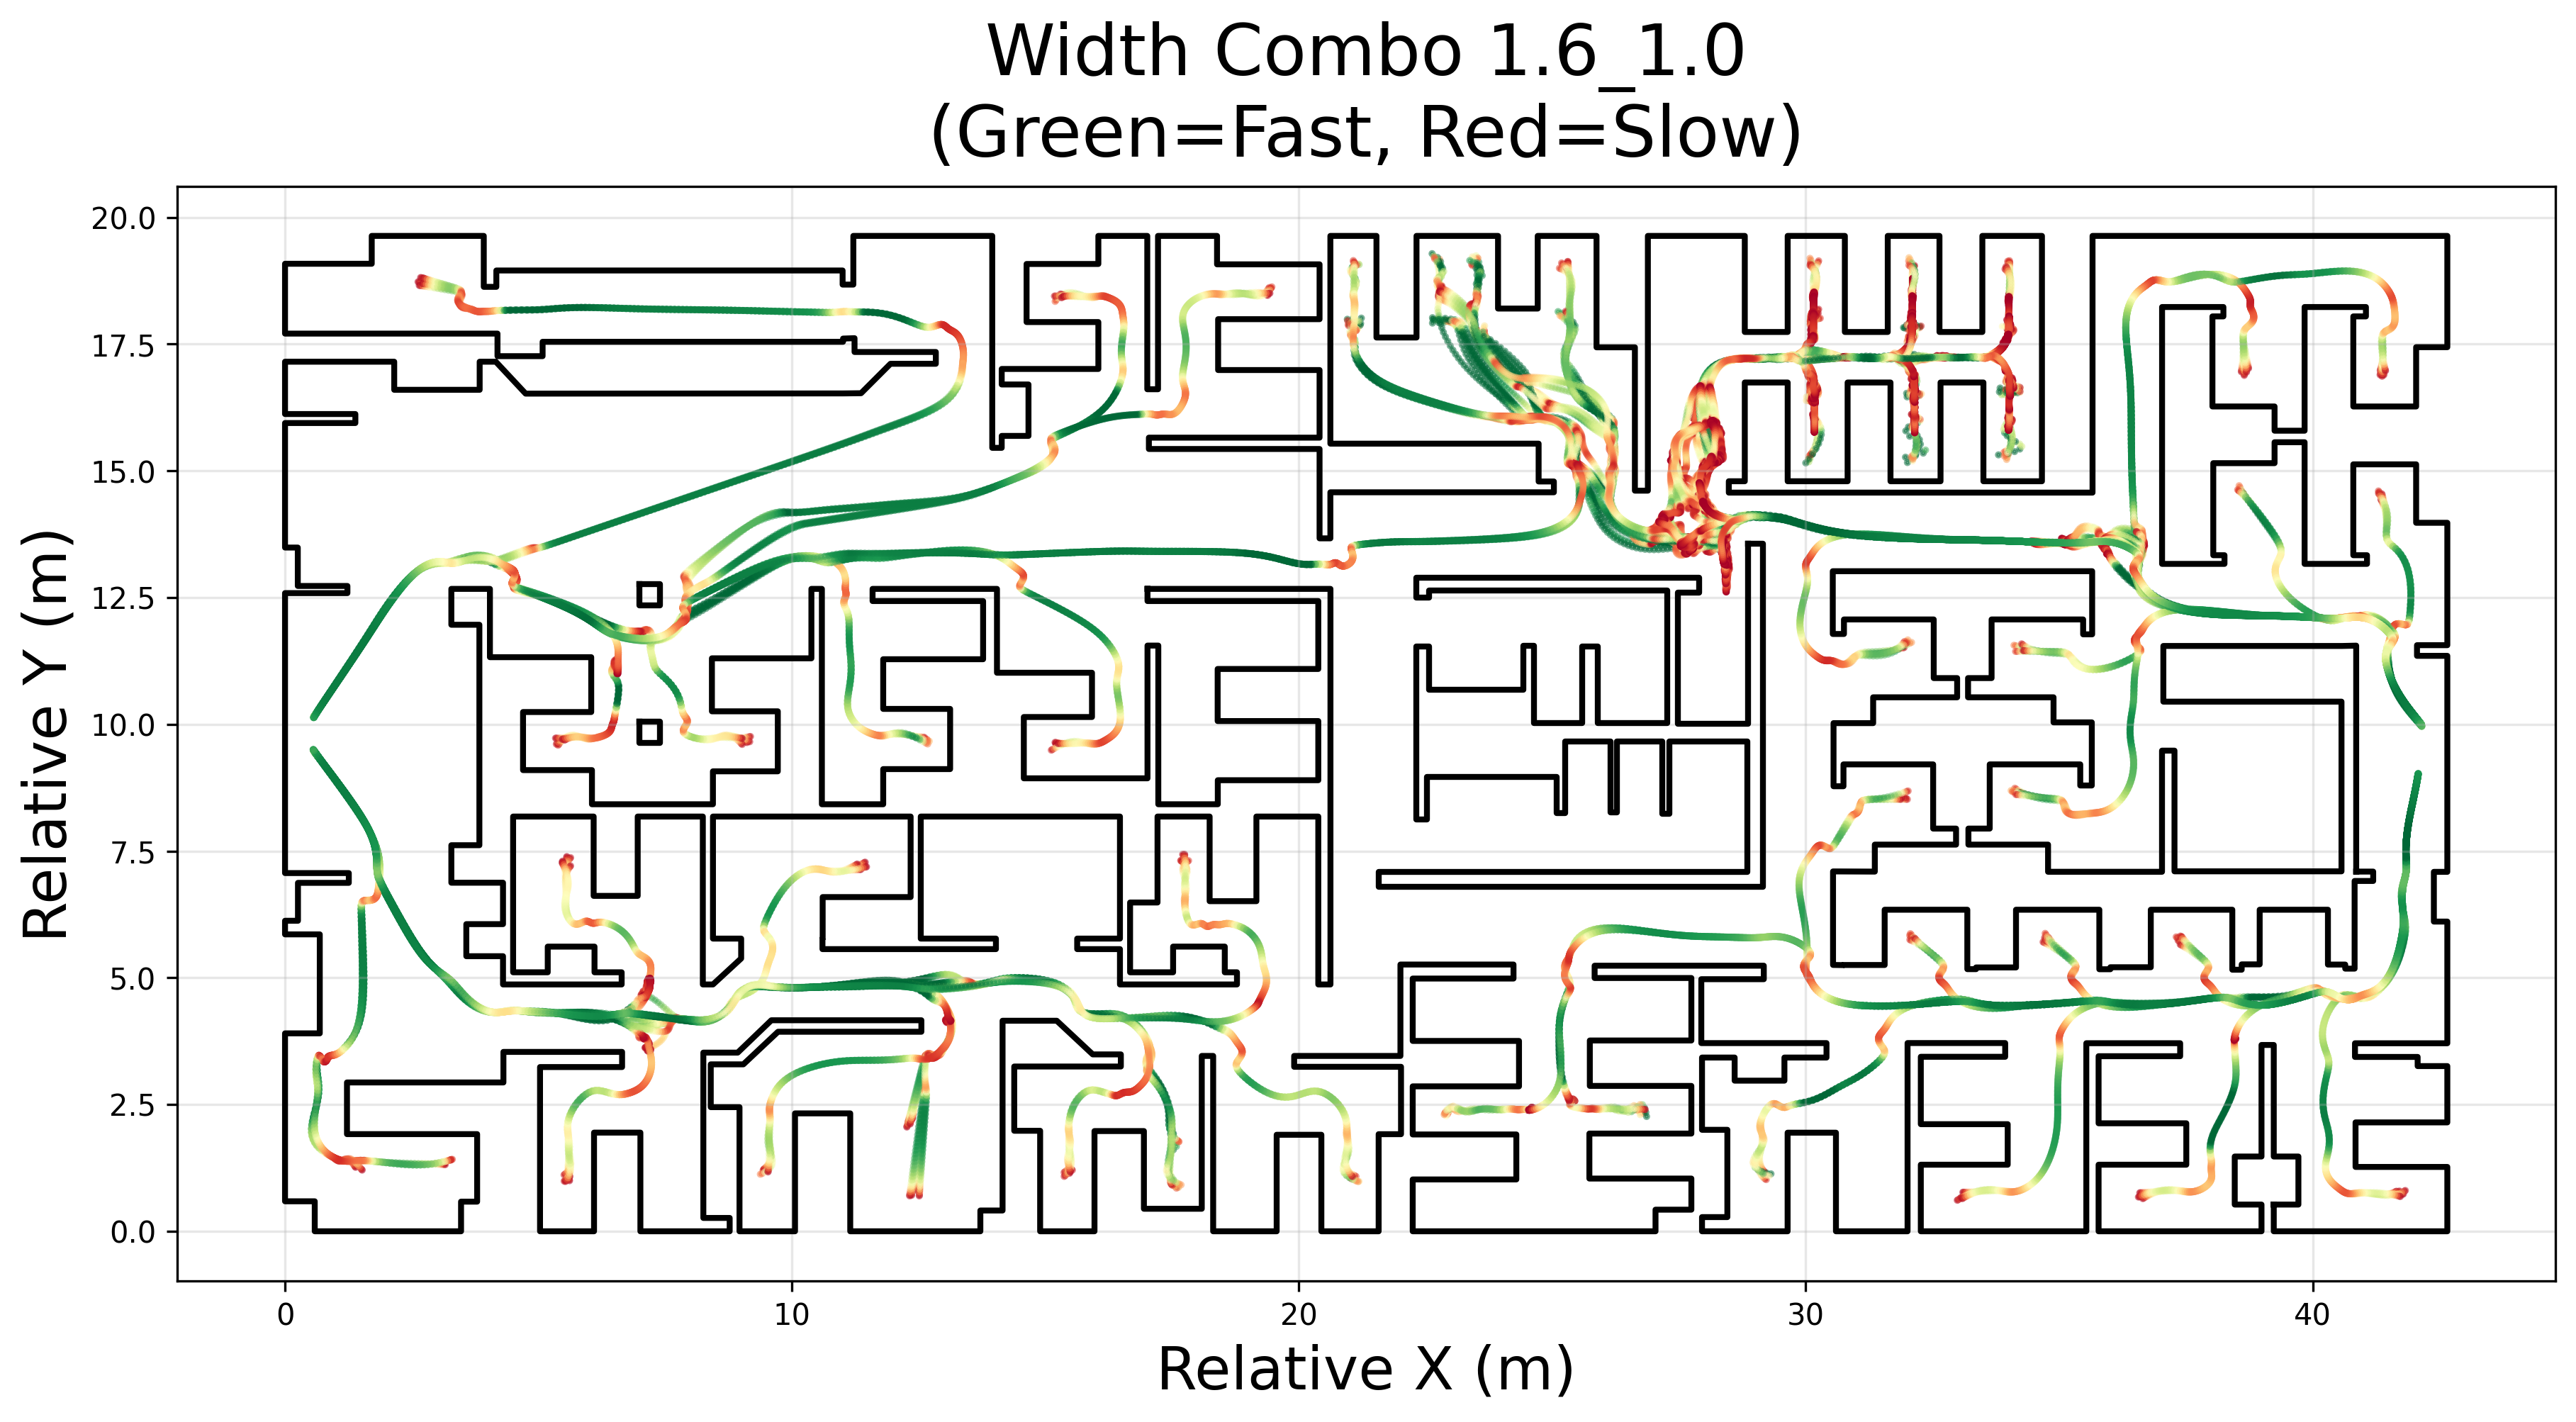
\includegraphics[width=\linewidth]{
            speed_trajectory_MultiRoom_width_1.6_1.0.png}
        \caption{Width Combo 1.6m and 1.0m}
        \label{fig:width_combo_1.6_1.0m}
    \end{subfigure}
    \begin{subfigure}[b]{.45\linewidth}
        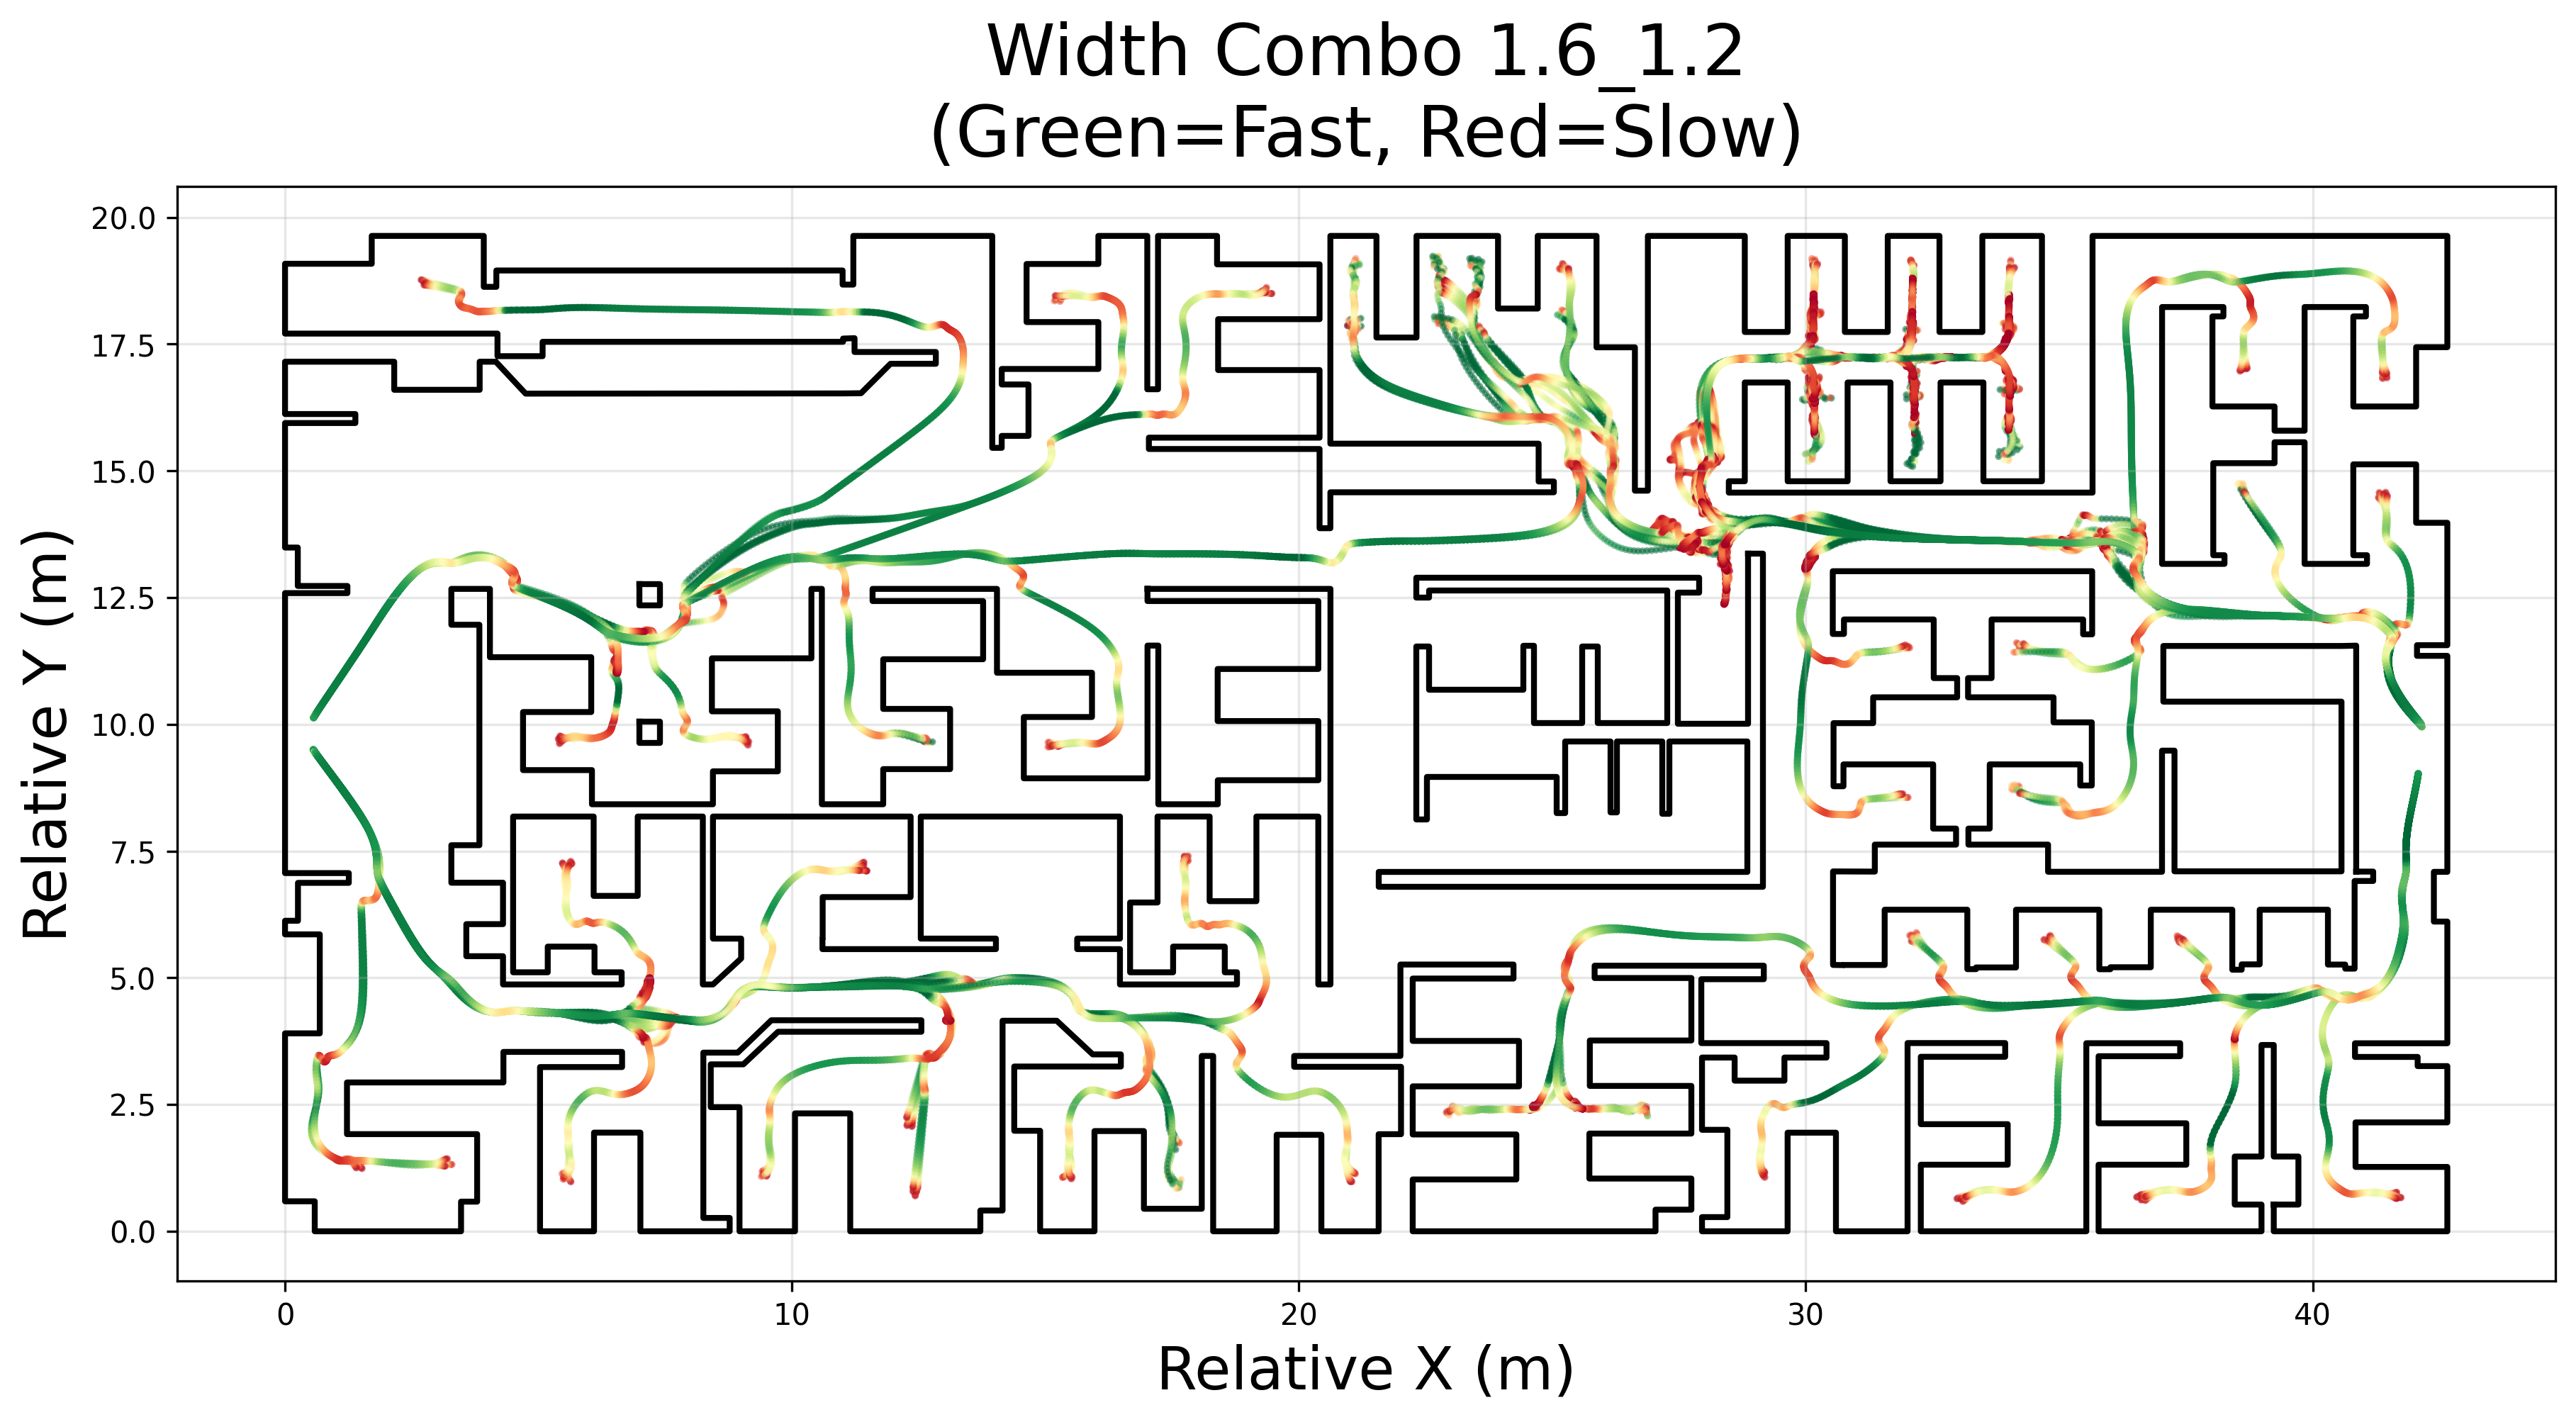
\includegraphics[width=\linewidth]{
            speed_trajectory_MultiRoom_width_1.6_1.2.png}
        \caption{Width Combo 1.6m and 1.2m}
        \label{fig:width_combo_1.6_1.2m}
    \end{subfigure}

    \begin{subfigure}[b]{.45\linewidth}
        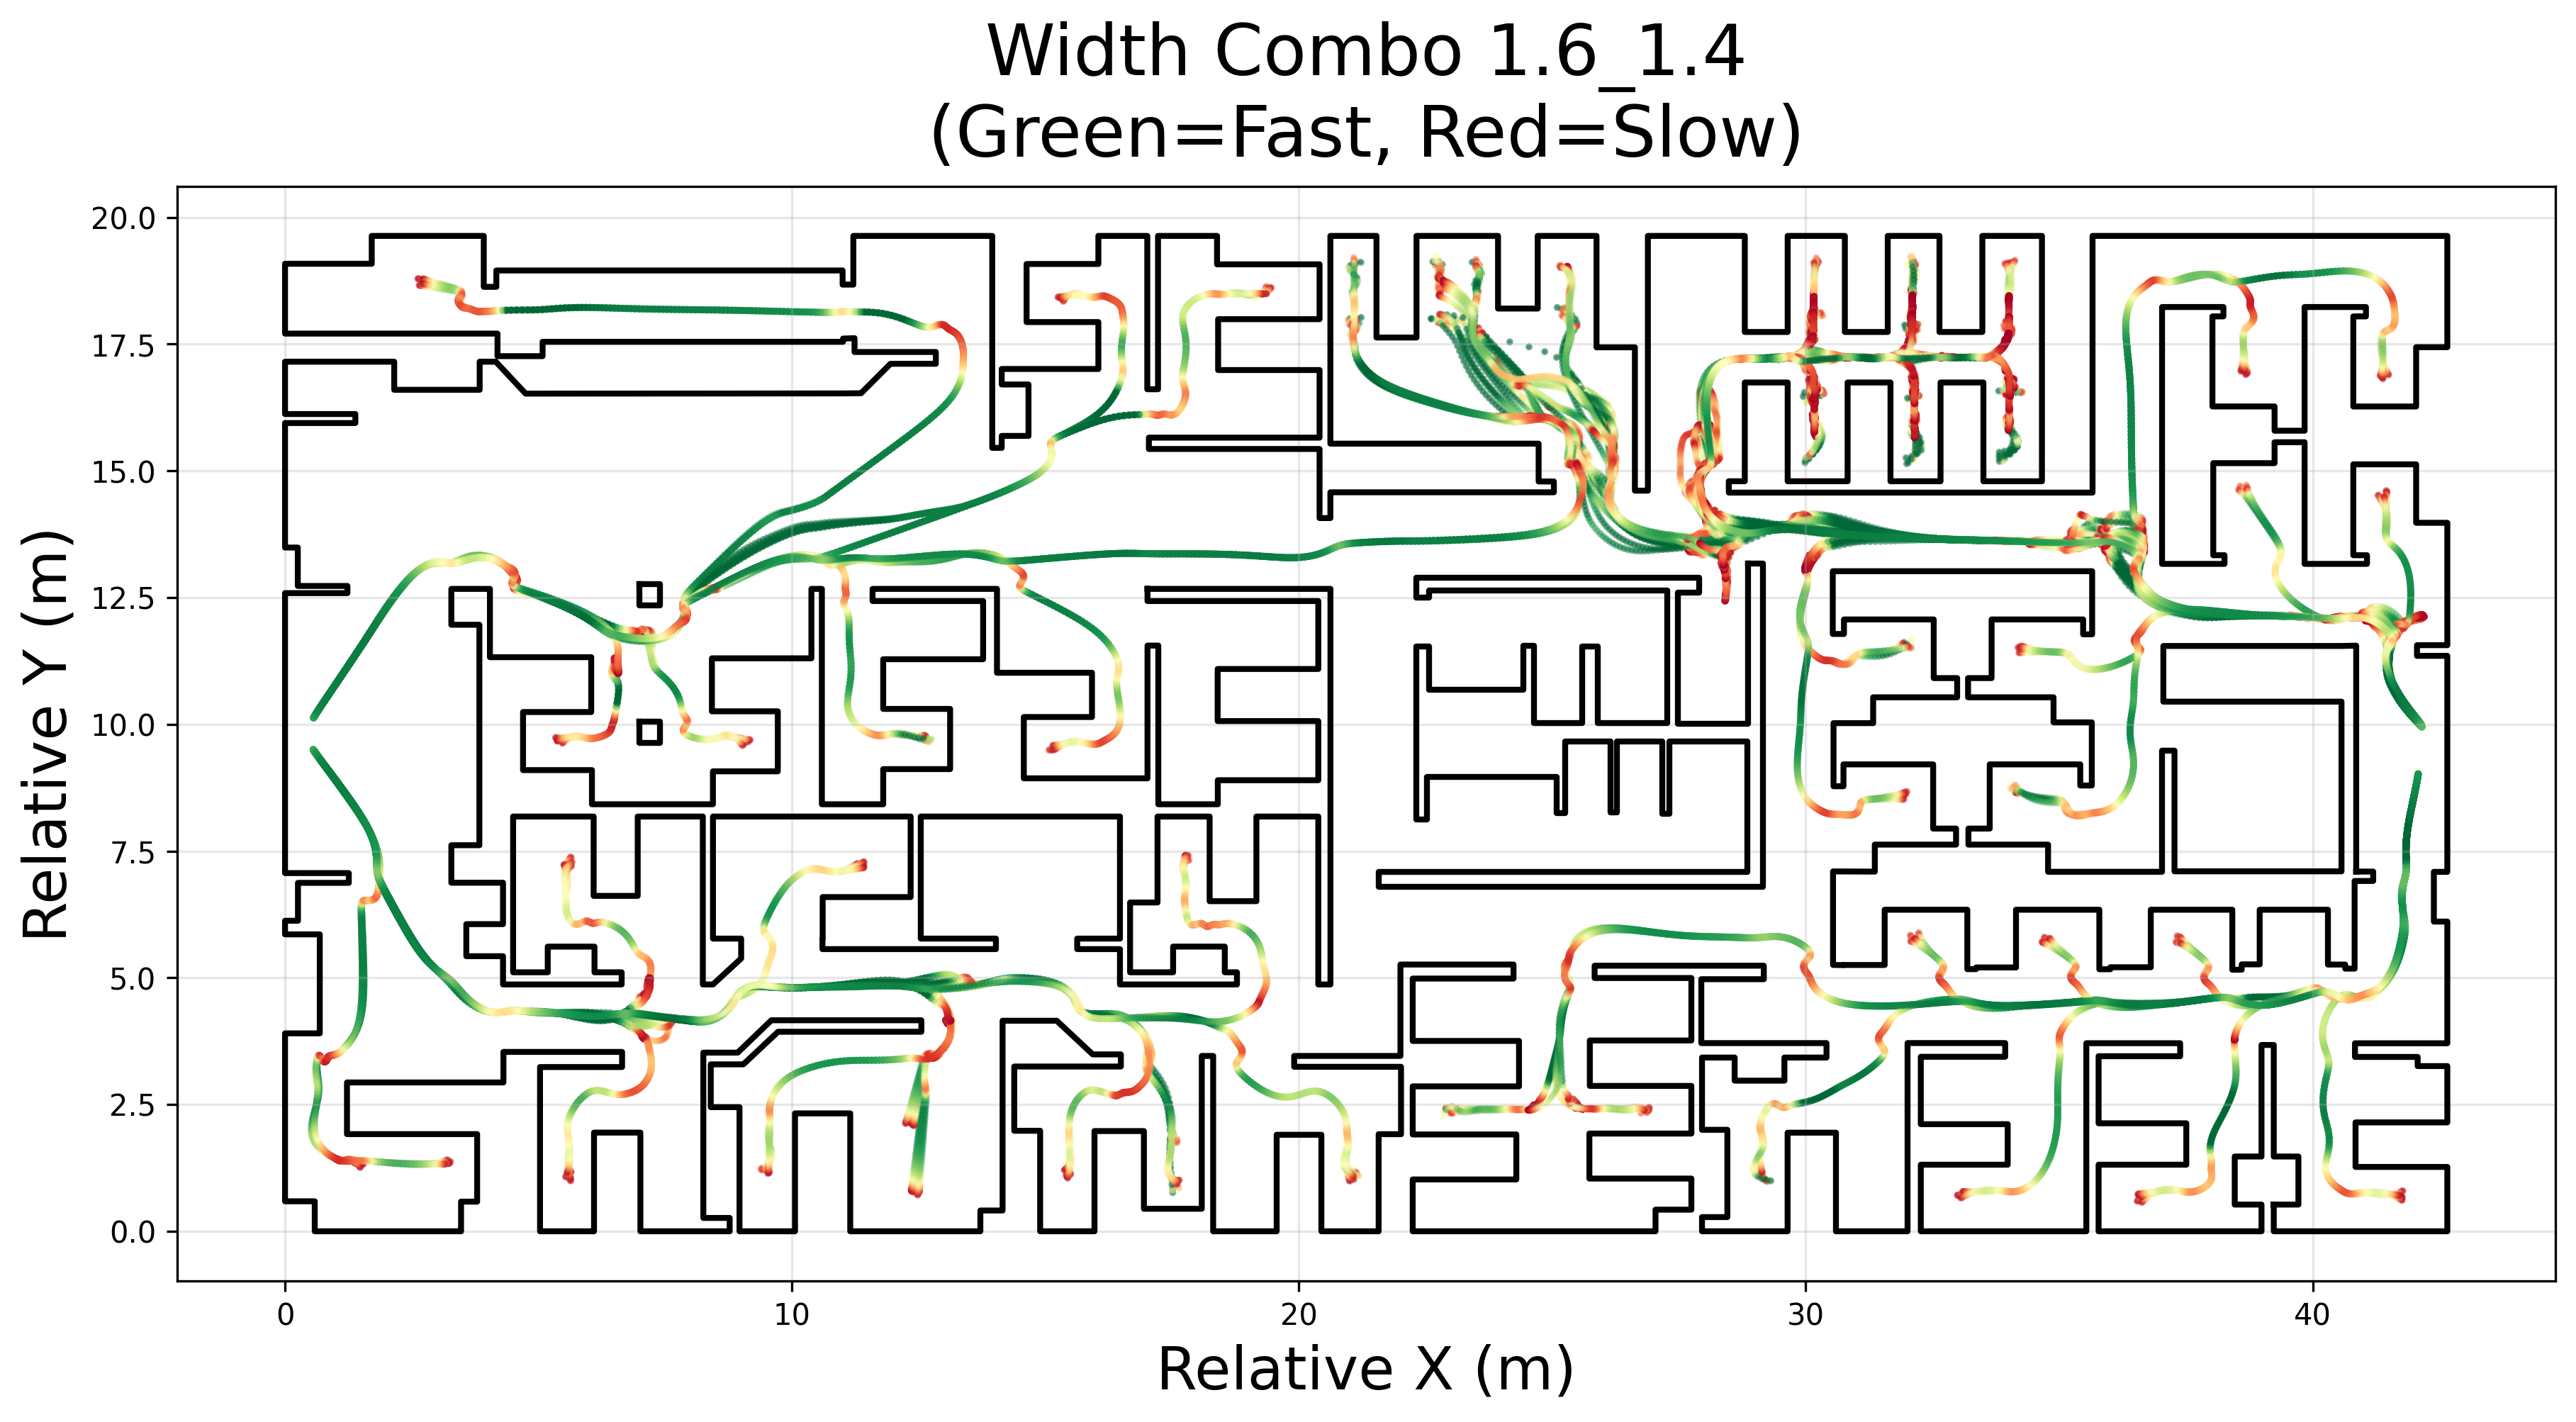
\includegraphics[width=\linewidth]{
            speed_trajectory_MultiRoom_width_1.6_1.4.png}
        \caption{Width Combo 1.6m and 1.4m}
        \label{fig:width_combo_1.6_1.4m}
    \end{subfigure}
        \begin{subfigure}[b]{.45\linewidth}
        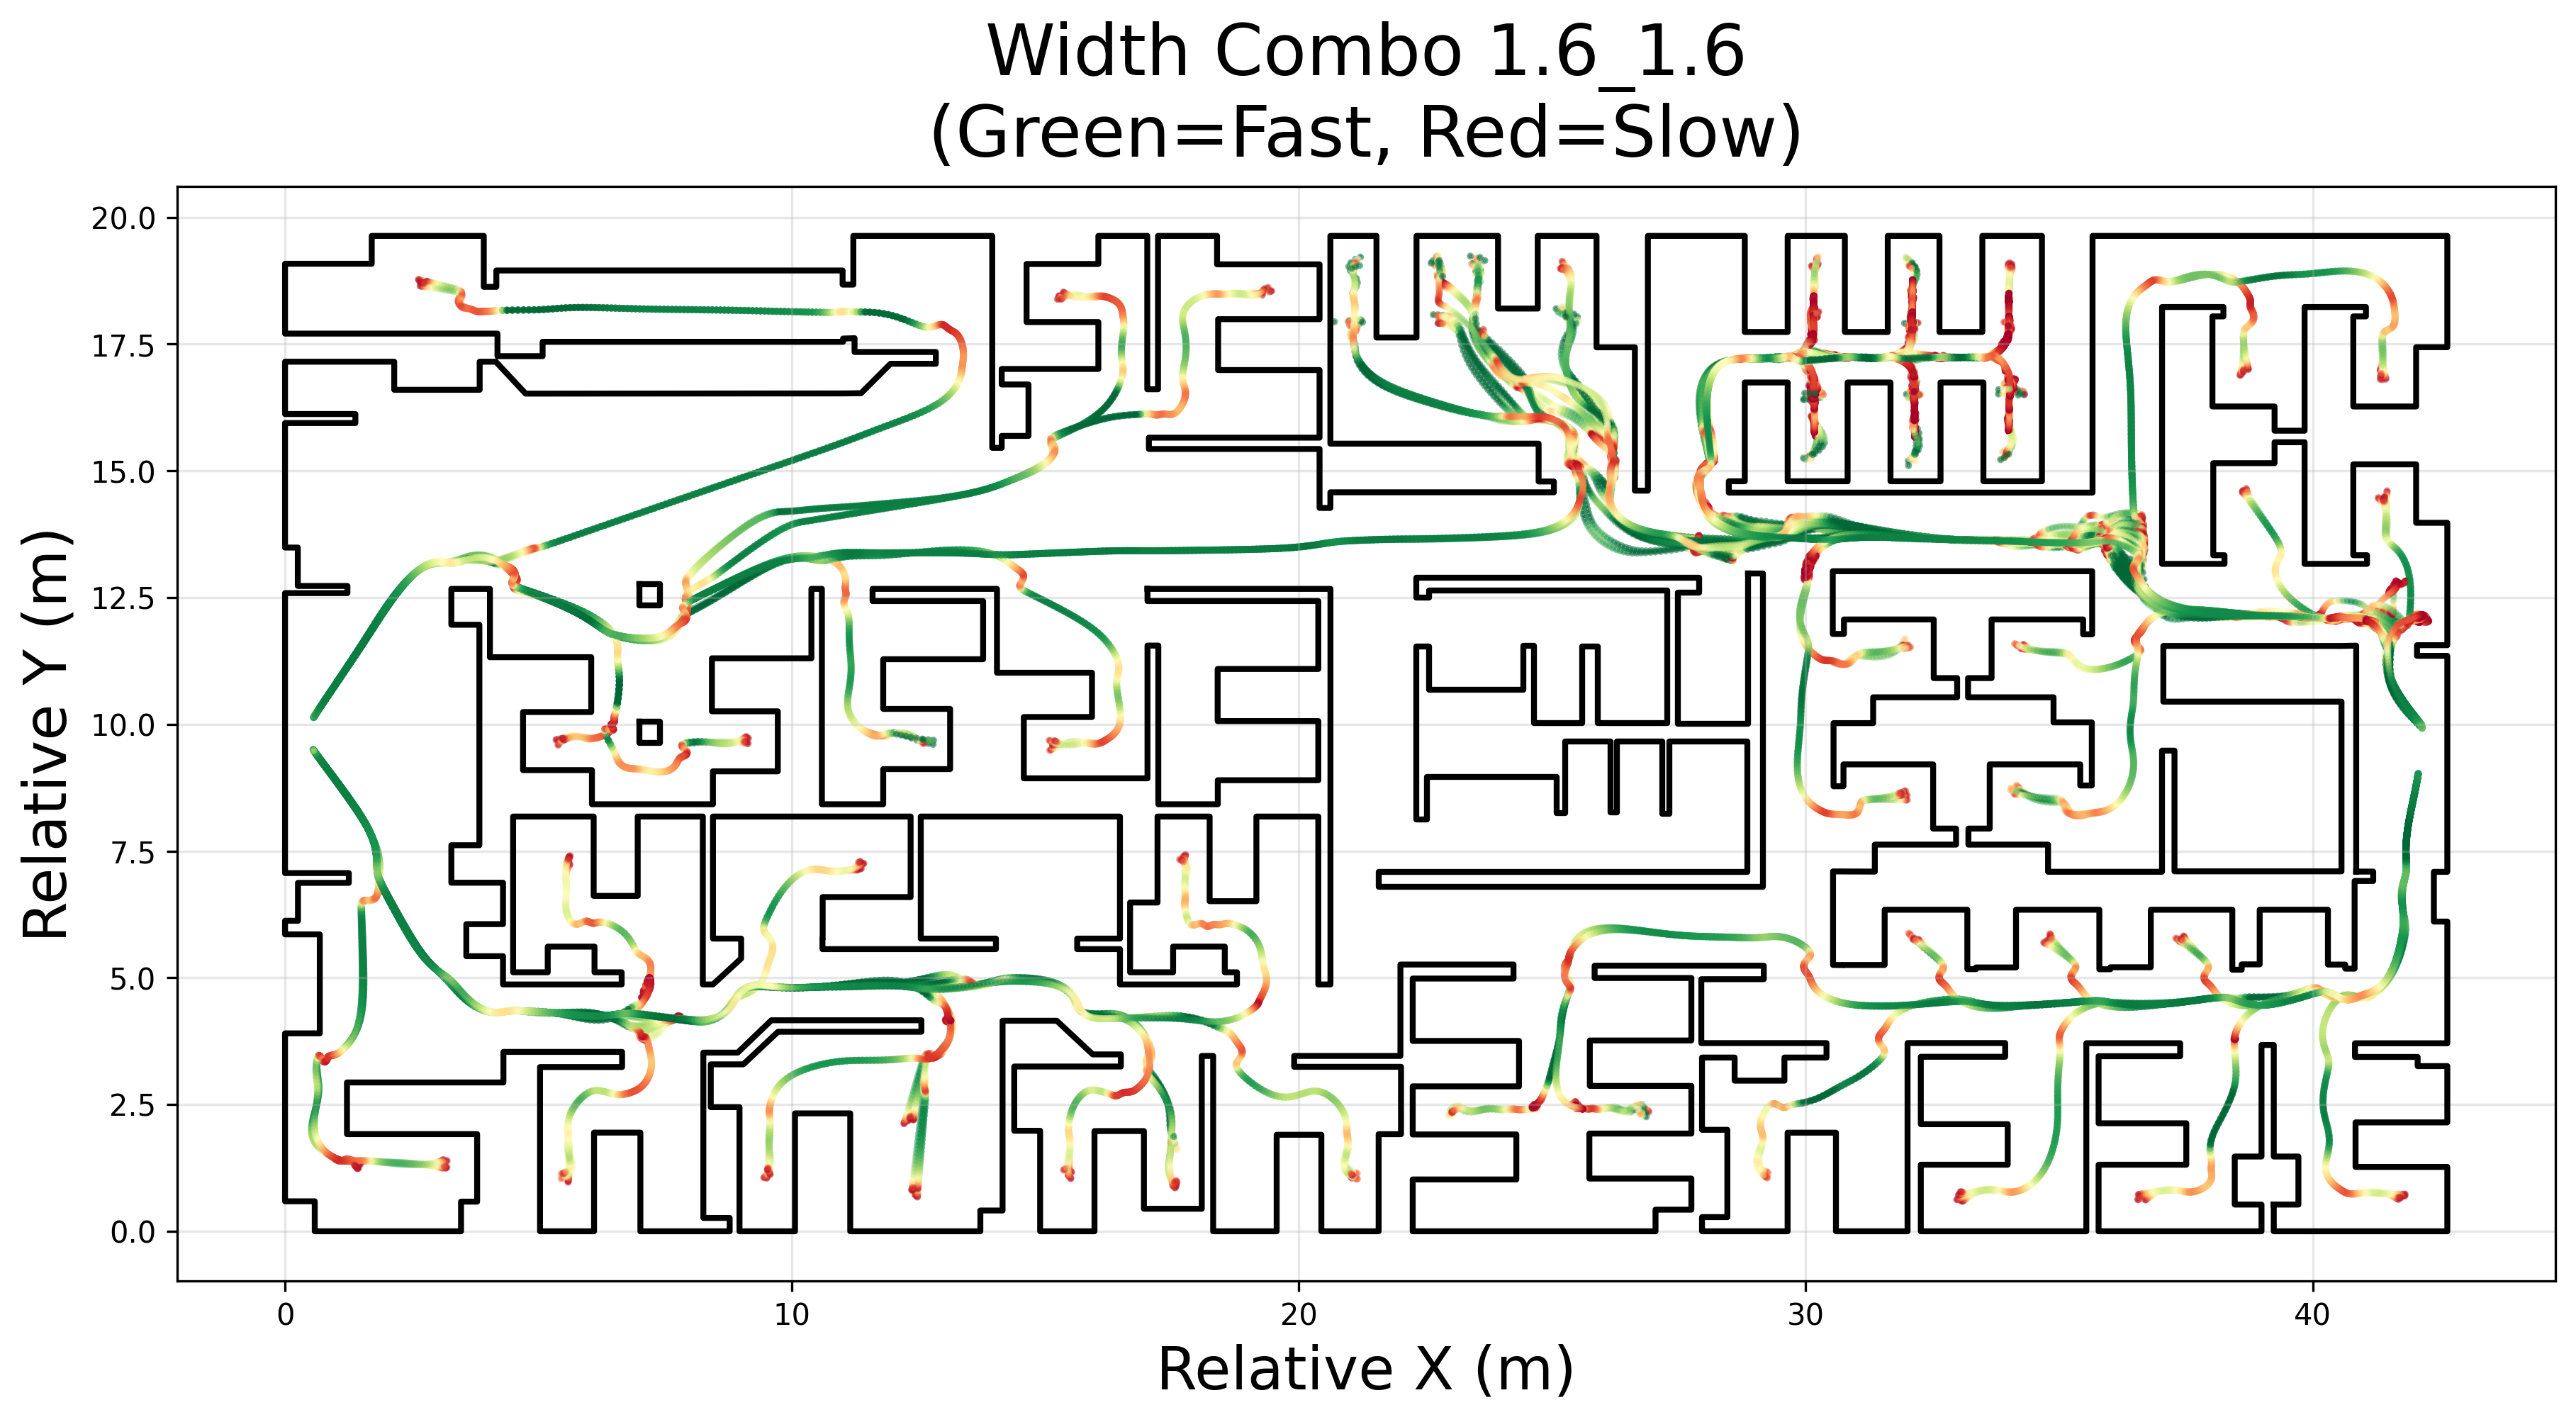
\includegraphics[width=\linewidth]{
            speed_trajectory_MultiRoom_width_1.6_1.6.png}
        \caption{Width Combo 1.6m and 1.6m}
        \label{fig:width_combo_1.6_1.6m}
    \end{subfigure}

    \caption{Speed and Trajectories for Room Door Width 1.6m}
    \label{fig:width_combo_1.6_x}
\end{figure}